% Chapter 2: Structural breaks and nonlinear models
% Advanced Time Series Analysis and Forecasting -- Master's programme Applied Statistics and Data Science, year 1, semester 2, Bucharest University of Economic Studies
% GENERATED by latex/build_chapter2.py -- edit the generator, not this file.

\newcommand{\coursename}{Advanced Time Series Analysis and Forecasting}
% Preambul comun ATS -- Analiza avansată a seriilor de timp și previziune / Advanced Time Series Analysis and Forecasting
% (Beamer, 16:9). Același design ca MFM, SFM și TSA (copiat din TSA, 5 octombrie 2026). Înainte de % Preambul comun ATS -- Analiza avansată a seriilor de timp și previziune / Advanced Time Series Analysis and Forecasting
% (Beamer, 16:9). Același design ca MFM, SFM și TSA (copiat din TSA, 5 octombrie 2026). Înainte de % Preambul comun ATS -- Analiza avansată a seriilor de timp și previziune / Advanced Time Series Analysis and Forecasting
% (Beamer, 16:9). Același design ca MFM, SFM și TSA (copiat din TSA, 5 octombrie 2026). Înainte de \input{../../latex/preamble} se definește
%   \newcommand{\coursename}{Advanced Time Series Analysis and Forecasting}          (EN)
%   \newcommand{\coursename}{Analiza avansată a seriilor de timp și previziune}       (RO)  și  \def\atslang{ro}
% Fișierele .tex se află în EN/Courses, EN/Seminars, RO/Cursuri, RO/Seminarii (două niveluri sub rădăcină).
% Deck-urile sînt generate de latex/build_chapterN.py / build_seminarN.py (vezi latex/ats_build.py).

\documentclass[9pt, aspectratio=169, t]{beamer}
\providecommand{\coursename}{Advanced Time Series Analysis and Forecasting}

% Ensure content fits on slides
\setbeamersize{text margin left=8mm, text margin right=8mm}
% Smaller institute font (title page)
\setbeamerfont{institute}{size=\footnotesize}

%=============================================================================
% THEME AND STYLE CONFIGURATION
%=============================================================================
\usetheme{default}
% Using default theme for clean header/footer control

% Color Palette (matching Redispatch PDF)
\definecolor{MainBlue}{RGB}{26, 58, 110}
\definecolor{AccentBlue}{RGB}{26, 58, 110}
\definecolor{IDAred}{RGB}{205, 0, 0}
\definecolor{DarkGray}{RGB}{51, 51, 51}
\definecolor{MediumGray}{RGB}{128, 128, 128}
\definecolor{LightGray}{RGB}{248, 248, 248}
\definecolor{VeryLightGray}{RGB}{235, 235, 235}
\definecolor{KeynoteGray}{RGB}{218, 218, 218}
\definecolor{SectionGray}{RGB}{120, 120, 120}
\definecolor{FooterGray}{RGB}{100, 100, 100}
\definecolor{Crimson}{RGB}{220, 53, 69}
\definecolor{Forest}{RGB}{46, 125, 50}
\definecolor{Amber}{RGB}{181, 133, 63}
\definecolor{Orange}{RGB}{230, 126, 34}
\definecolor{Purple}{RGB}{142, 68, 173}

% Gradient background (exact Keynote 315° gradient: white to RGB 218,218,218)
\setbeamertemplate{background}{%
    \begin{tikzpicture}[remember picture, overlay]
        \shade[shading=axis, shading angle=315,
        top color=white, bottom color=KeynoteGray]
        (current page.south west) rectangle (current page.north east);
    \end{tikzpicture}%
}
% Fallback solid color for compatibility
\setbeamercolor{background canvas}{bg=}

\setbeamercolor{palette primary}{bg=MainBlue, fg=white}
\setbeamercolor{palette secondary}{bg=MainBlue!85, fg=white}
\setbeamercolor{palette tertiary}{bg=MainBlue!70, fg=white}
\setbeamercolor{structure}{fg=MainBlue}
\setbeamercolor{title}{fg=IDAred}
\setbeamercolor{frametitle}{fg=IDAred, bg=}
\setbeamercolor{block title}{bg=MainBlue, fg=white}
\setbeamercolor{block body}{bg=VeryLightGray, fg=DarkGray}
\setbeamercolor{block title alerted}{bg=Crimson, fg=white}
\setbeamercolor{block body alerted}{bg=Crimson!8, fg=DarkGray}
\setbeamercolor{block title example}{bg=Forest, fg=white}
\setbeamercolor{block body example}{bg=Forest!8, fg=DarkGray}
\setbeamercolor{item}{fg=MainBlue}

% Footer colors (override Madrid theme blue)
\setbeamercolor{author in head/foot}{fg=FooterGray, bg=}
\setbeamercolor{title in head/foot}{fg=FooterGray, bg=}
\setbeamercolor{date in head/foot}{fg=FooterGray, bg=}
\setbeamercolor{section in head/foot}{fg=FooterGray, bg=}
\setbeamercolor{subsection in head/foot}{fg=FooterGray, bg=}

% Bullet styles (apply everywhere including blocks)
\setbeamertemplate{itemize item}{\color{MainBlue}$\boxdot$}
\setbeamertemplate{itemize subitem}{\color{MainBlue}$\blacktriangleright$}
\setbeamertemplate{itemize subsubitem}{\color{MainBlue}\tiny$\bullet$}
\setbeamertemplate{itemize/enumerate body begin}{\normalsize}
\setbeamertemplate{itemize/enumerate subbody begin}{\normalsize}

% Item spacing - compact style
\setlength{\leftmargini}{10pt}       % Level 1: minimal indent
\setlength{\leftmarginii}{10pt}      % Level 2: minimal additional indent
% Compact list spacing (zero extra space before/after lists in blocks)
\makeatletter
\def\@listi{\leftmargin\leftmargini \topsep 0pt \parsep 0pt \itemsep 0pt}
\def\@listii{\leftmargin\leftmarginii \topsep 0pt \parsep 0pt \itemsep 0pt}
\makeatother

\setbeamertemplate{navigation symbols}{}

%=============================================================================
% CUSTOM HEADLINE
%=============================================================================
\setbeamertemplate{headline}{%
    \vskip10pt%
    \hbox to \paperwidth{%
        \hskip0.5cm%
        {\small\color{FooterGray}\renewcommand{\hyperlink}[2]{##2}\insertsectionhead}%
        \hfill%
        \textcolor{FooterGray}{\small\insertframenumber}%
        \hskip0.5cm%
    }%
    \vskip4pt%
    {\color{FooterGray}\hrule height 0.4pt}%
}

%=============================================================================
% CUSTOM FOOTER
%=============================================================================
\usepackage{fontawesome5}

\setbeamertemplate{footline}{%
    {\color{FooterGray}\hrule height 0.4pt}%
    \vskip4pt%
    \hbox to \paperwidth{%
        \hskip0.5cm%
        \textcolor{FooterGray}{\small\coursename}%
        \hfill%
        \raisebox{-0.1em}{%
            \begin{tikzpicture}[x=0.08em, y=0.08em, line width=0.4pt]
                \draw[FooterGray] (0,3) -- (1,4) -- (2,3.5) -- (3,5) -- (4,4) -- (5,6) -- (6,5.5) -- (7,4) -- (8,5) -- (9,7) -- (10,6) -- (11,5) -- (12,6.5) -- (13,8) -- (14,7) -- (15,6) -- (16,7.5) -- (17,9) -- (18,8) -- (19,7) -- (20,8.5) -- (21,10) -- (22,9) -- (23,8) -- (24,9.5);
            \end{tikzpicture}%
        }%
        \hskip0.5cm%
    }%
    \vskip6pt%
}

%=============================================================================
% PACKAGES
%=============================================================================
\usepackage[utf8]{inputenc}
\DeclareUnicodeCharacter{03B1}{\ensuremath{\alpha}}
\usepackage[T1]{fontenc}
\usepackage{amsmath, amssymb, amsthm}
\usepackage{mathtools}
\usepackage{bm}
\usepackage{tikz}
\usetikzlibrary{arrows.meta, positioning, shapes, calc, decorations.pathreplacing, shadings}
\usepackage{booktabs}
\usepackage{multirow}
\usepackage{array}
\usepackage{graphicx}
\usepackage{animate}
\usepackage{hyperref}
\usepackage{colortbl}
\usepackage{listings}
\lstset{language=Python, basicstyle=\ttfamily\scriptsize, keywordstyle=\color{MainBlue}\bfseries,
  commentstyle=\color{Forest}, stringstyle=\color{Crimson}, breaklines=true,
  frame=none, backgroundcolor=\color{VeryLightGray}, xleftmargin=2mm}
\hypersetup{colorlinks=true, linkcolor=MainBlue, urlcolor=MainBlue}
\graphicspath{{../../logos/}{../../charts/}{../../photos/}}
\usepackage{xcolor}
\hfuzz=2pt  % Suppress tiny overfull warnings (<2pt)
\vfuzz=2pt  % Suppress tiny vertical overfull warnings (<2pt)

%=============================================================================
% QUANTLET COMMANDS
%   \quantlet{<displayed name>}{<url>}       (generic)
%   \atsquantlet{Ch_05}{ATS_ch5_garch}       -> https://github.com/danpele/Advanced-Time-Series/tree/main/Quantlets/Ch_05/ATS_ch5_garch
%   \qlurl{<folder>} is defined per chapter by the generator (Quantlets/Ch_NN/<folder>)
%=============================================================================
\newcommand{\atsrepo}{https://github.com/danpele/Advanced-Time-Series}
\newcommand{\atsqlbase}{https://github.com/danpele/Advanced-Time-Series/tree/main/Quantlets}
\newcommand{\quantlet}[2]{%
    \hfill\href{#2}{%
        \raisebox{-0.15em}{
\includegraphics[height=0.7em]{ql_logo.png}}%
        \textcolor{MainBlue}{\tiny\ #1}%
    }%
}
\newcommand{\atsquantlet}[2]{\quantlet{\detokenize{#2}}{\atsqlbase/#1/#2}}

%=============================================================================
% NOTEBOOKS (Google Colab)
%   \colaburl{notebooks/EN/chapter5_seminar_notebook.ipynb} -> the Colab link of a file in the ATS repo
%   \nb: the chapter notebook (each seminar deck redefines it with \renewcommand)
%=============================================================================
\newcommand{\colaburl}[1]{https://colab.research.google.com/github/danpele/Advanced-Time-Series/blob/main/#1}
\newcommand{\nb}{https://colab.research.google.com/github/danpele/Advanced-Time-Series/tree/main/notebooks/EN}
\newcommand{\nbname}{notebooks/EN}

%=============================================================================
% SLIDE HELPERS (used by the generators; the same as in MFM)
%=============================================================================
% local font size for list bodies (the preamble forces \normalsize)
\newcommand{\itemsize}[1]{\setbeamertemplate{itemize/enumerate body begin}{#1}\setbeamertemplate{itemize/enumerate subbody begin}{#1}}
\newcommand{\intitle}[1]{{\hypersetup{urlcolor=white}#1}}   % white links inside coloured title bars
\newcommand{\imgcap}[1]{{\scriptsize #1}\\[0.5mm]}          % caption under a photo
\newcommand{\imgcredit}[2]{{\tiny\color{FooterGray}\href{#1}{#2}}}   % image credit: source URL, author/licence
\newcommand{\aiprompt}[1]{{\ttfamily\color{MainBlue}#1}}     % a prompt to an AI assistant

%=============================================================================
% SEMINARS: student version by default; the instructor wrapper *_solutions.tex sets \solutionstrue
%=============================================================================
\makeatletter\@ifundefined{ifsolutions}{\expandafter\newif\csname ifsolutions\endcsname}{}\makeatother
\newcommand{\solonly}[1]{\ifsolutions #1\fi}
\newcommand{\propsub}{\ifsolutions\else\framesubtitle{\ifdefined\atslang Rezolvarea se discută la seminar\else Solution discussed in class\fi}\fi}

%=============================================================================
% APPENDIX AND CHAPTER LINKS (latex/appendix_links.py writes the calls; it also re-declares these
% macros before \begin{document}, so the decks compile with or without this preamble block)
%=============================================================================
\providecommand{\atsapplink}[3]{\hypertarget{#2}{}\hyperlink{#1}{\beamergotobutton{#3}}}
\providecommand{\atsappback}[2]{\begin{tikzpicture}[remember picture,overlay]\node[anchor=south east] at ([xshift=-3mm,yshift=7mm]current page.south east){\hyperlink{#1}{\beamerreturnbutton{#2}}};\end{tikzpicture}}
\providecommand{\atschlink}[2]{\href{#1}{#2}}
\providecommand{\atschlinkt}[2]{\href{#1}{\usebeamercolor[fg]{frametitle}#2}}

%=============================================================================
% QUANTINAR COMMAND: link către un curs Quantinar (subiecte avansate)
%=============================================================================
\newcommand{\quantinar}[2]{%
    \href{#2}{%
        \raisebox{-0.15em}{
\includegraphics[height=0.8em]{qr_logo.png}}%
        \textcolor{MainBlue}{\scriptsize\ #1}%
    }%
}

%=============================================================================
% CUSTOM TITLE PAGE
%=============================================================================
\defbeamertemplate*{title page}{hybrid}[1][]
{
    \vspace{0.2cm}
    % Logos row - top header (with clickable links)
    \begin{center}
        \href{https://www.ase.ro}{
\includegraphics[height=1.0cm]{ase_logo.png}}\hspace{0.3cm}%
        \href{https://theida.net}{
\includegraphics[height=1.0cm]{ida_logo.png}}\hspace{0.3cm}%
        \href{https://blockchain-research-center.com}{
\includegraphics[height=1.0cm]{brc_logo.png}}\hspace{0.3cm}%
        \href{https://www.ai4efin.ase.ro}{
\includegraphics[height=1.0cm]{ai4efin_logo.png}}\hspace{0.3cm}%
        \href{https://ipe.ro/new}{
\includegraphics[height=1.0cm]{acad_logo.png}}\hspace{0.3cm}%
        \href{https://www.digital-finance-msca.com}{
\includegraphics[height=1.0cm]{msca_logo.png}}%
    \end{center}

    \vspace{0.6cm}

    % Main title with Q logos on sides (with clickable links)
    \begin{center}
        \begin{minipage}{0.1\textwidth}
            \centering
            \href{https://quantlet.com}{
\includegraphics[height=1.1cm]{ql_logo.png}}
        \end{minipage}%
        \begin{minipage}{0.78\textwidth}
            \centering
            {\LARGE\bfseries\usebeamercolor[fg]{title}\inserttitle}

            \vspace{0.3cm}

            {\usebeamerfont{subtitle}\usebeamercolor[fg]{title}\insertsubtitle}
        \end{minipage}%
        \begin{minipage}{0.1\textwidth}
            \centering
            \href{https://quantinar.com}{
\includegraphics[height=1.1cm]{qr_logo.png}}
        \end{minipage}
    \end{center}

    \vspace{0.6cm}

    % Authors (left aligned)
    \hspace{0.5cm}{\usebeamerfont{author}\insertauthor}

    \vspace{0.3cm}

    % Institute/Affiliations (left aligned)
    \hspace{0.5cm}\begin{minipage}[t]{0.9\textwidth}
        \raggedright\small\insertinstitute
    \end{minipage}
}

%=============================================================================
% THEOREM ENVIRONMENTS
%=============================================================================
\theoremstyle{definition}
\setbeamertemplate{theorems}[numbered]
\ifdefined\atslang
\newtheorem{defn}{Definiție}
\newtheorem{thm}{Teoremă}
\newtheorem{prop}{Propoziție}
\newtheorem{rmk}{Observație}
\else
\newtheorem{defn}{Definition}
\newtheorem{thm}{Theorem}
\newtheorem{prop}{Proposition}
\newtheorem{rmk}{Remark}
\fi

%=============================================================================
% CENTRED MINIPAGE (no extra vertical space)
%=============================================================================
\newenvironment{cminipage}[1]{%
    \par\noindent\hfill\begin{minipage}{#1}\ignorespaces
}{%
    \end{minipage}\hfill\null\par
}

%=============================================================================
% CUSTOM COMMANDS
%=============================================================================
\newcommand{\E}{\mathbb{E}}
\newcommand{\Var}{\text{Var}}
\newcommand{\Cov}{\text{Cov}}
\newcommand{\Corr}{\text{Corr}}
\newcommand{\R}{\mathbb{R}}
\newcommand{\N}{\mathbb{N}}
\newcommand{\Z}{\mathbb{Z}}
\newcommand{\B}{\mathbf{B}}
\newcommand{\imark}{\textcolor{MainBlue}{\textbullet}}
\newcommand{\RMSE}{\text{RMSE}}
\newcommand{\MAE}{\text{MAE}}
\newcommand{\MAPE}{\text{MAPE}}

% Boldface vector/matrix commands (VAR, VECM, state space)
\newcommand{\bY}{\mathbf{Y}}
\newcommand{\bX}{\mathbf{X}}
\newcommand{\bA}{\mathbf{A}}
\newcommand{\bB}{\mathbf{B}}
\newcommand{\bepsilon}{\boldsymbol{\varepsilon}}
\newcommand{\bSigma}{\boldsymbol{\Sigma}}
\newcommand{\bPhi}{\boldsymbol{\Phi}}
\newcommand{\bGamma}{\boldsymbol{\Gamma}}
\newcommand{\bPi}{\boldsymbol{\Pi}}
\newcommand{\bc}{\mathbf{c}}
\newcommand{\balpha}{\boldsymbol{\alpha}}
\newcommand{\bbeta}{\boldsymbol{\beta}}
\newcommand{\bvarepsilon}{\boldsymbol{\varepsilon}}

% Seminar marks
\newcommand{\correct}{\textcolor{Forest}{\checkmark}}
\newcommand{\incorrect}{\textcolor{Crimson}{\texttimes}}
 se definește
%   \newcommand{\coursename}{Advanced Time Series Analysis and Forecasting}          (EN)
%   \newcommand{\coursename}{Analiza avansată a seriilor de timp și previziune}       (RO)  și  \def\atslang{ro}
% Fișierele .tex se află în EN/Courses, EN/Seminars, RO/Cursuri, RO/Seminarii (două niveluri sub rădăcină).
% Deck-urile sînt generate de latex/build_chapterN.py / build_seminarN.py (vezi latex/ats_build.py).

\documentclass[9pt, aspectratio=169, t]{beamer}
\providecommand{\coursename}{Advanced Time Series Analysis and Forecasting}

% Ensure content fits on slides
\setbeamersize{text margin left=8mm, text margin right=8mm}
% Smaller institute font (title page)
\setbeamerfont{institute}{size=\footnotesize}

%=============================================================================
% THEME AND STYLE CONFIGURATION
%=============================================================================
\usetheme{default}
% Using default theme for clean header/footer control

% Color Palette (matching Redispatch PDF)
\definecolor{MainBlue}{RGB}{26, 58, 110}
\definecolor{AccentBlue}{RGB}{26, 58, 110}
\definecolor{IDAred}{RGB}{205, 0, 0}
\definecolor{DarkGray}{RGB}{51, 51, 51}
\definecolor{MediumGray}{RGB}{128, 128, 128}
\definecolor{LightGray}{RGB}{248, 248, 248}
\definecolor{VeryLightGray}{RGB}{235, 235, 235}
\definecolor{KeynoteGray}{RGB}{218, 218, 218}
\definecolor{SectionGray}{RGB}{120, 120, 120}
\definecolor{FooterGray}{RGB}{100, 100, 100}
\definecolor{Crimson}{RGB}{220, 53, 69}
\definecolor{Forest}{RGB}{46, 125, 50}
\definecolor{Amber}{RGB}{181, 133, 63}
\definecolor{Orange}{RGB}{230, 126, 34}
\definecolor{Purple}{RGB}{142, 68, 173}

% Gradient background (exact Keynote 315° gradient: white to RGB 218,218,218)
\setbeamertemplate{background}{%
    \begin{tikzpicture}[remember picture, overlay]
        \shade[shading=axis, shading angle=315,
        top color=white, bottom color=KeynoteGray]
        (current page.south west) rectangle (current page.north east);
    \end{tikzpicture}%
}
% Fallback solid color for compatibility
\setbeamercolor{background canvas}{bg=}

\setbeamercolor{palette primary}{bg=MainBlue, fg=white}
\setbeamercolor{palette secondary}{bg=MainBlue!85, fg=white}
\setbeamercolor{palette tertiary}{bg=MainBlue!70, fg=white}
\setbeamercolor{structure}{fg=MainBlue}
\setbeamercolor{title}{fg=IDAred}
\setbeamercolor{frametitle}{fg=IDAred, bg=}
\setbeamercolor{block title}{bg=MainBlue, fg=white}
\setbeamercolor{block body}{bg=VeryLightGray, fg=DarkGray}
\setbeamercolor{block title alerted}{bg=Crimson, fg=white}
\setbeamercolor{block body alerted}{bg=Crimson!8, fg=DarkGray}
\setbeamercolor{block title example}{bg=Forest, fg=white}
\setbeamercolor{block body example}{bg=Forest!8, fg=DarkGray}
\setbeamercolor{item}{fg=MainBlue}

% Footer colors (override Madrid theme blue)
\setbeamercolor{author in head/foot}{fg=FooterGray, bg=}
\setbeamercolor{title in head/foot}{fg=FooterGray, bg=}
\setbeamercolor{date in head/foot}{fg=FooterGray, bg=}
\setbeamercolor{section in head/foot}{fg=FooterGray, bg=}
\setbeamercolor{subsection in head/foot}{fg=FooterGray, bg=}

% Bullet styles (apply everywhere including blocks)
\setbeamertemplate{itemize item}{\color{MainBlue}$\boxdot$}
\setbeamertemplate{itemize subitem}{\color{MainBlue}$\blacktriangleright$}
\setbeamertemplate{itemize subsubitem}{\color{MainBlue}\tiny$\bullet$}
\setbeamertemplate{itemize/enumerate body begin}{\normalsize}
\setbeamertemplate{itemize/enumerate subbody begin}{\normalsize}

% Item spacing - compact style
\setlength{\leftmargini}{10pt}       % Level 1: minimal indent
\setlength{\leftmarginii}{10pt}      % Level 2: minimal additional indent
% Compact list spacing (zero extra space before/after lists in blocks)
\makeatletter
\def\@listi{\leftmargin\leftmargini \topsep 0pt \parsep 0pt \itemsep 0pt}
\def\@listii{\leftmargin\leftmarginii \topsep 0pt \parsep 0pt \itemsep 0pt}
\makeatother

\setbeamertemplate{navigation symbols}{}

%=============================================================================
% CUSTOM HEADLINE
%=============================================================================
\setbeamertemplate{headline}{%
    \vskip10pt%
    \hbox to \paperwidth{%
        \hskip0.5cm%
        {\small\color{FooterGray}\renewcommand{\hyperlink}[2]{##2}\insertsectionhead}%
        \hfill%
        \textcolor{FooterGray}{\small\insertframenumber}%
        \hskip0.5cm%
    }%
    \vskip4pt%
    {\color{FooterGray}\hrule height 0.4pt}%
}

%=============================================================================
% CUSTOM FOOTER
%=============================================================================
\usepackage{fontawesome5}

\setbeamertemplate{footline}{%
    {\color{FooterGray}\hrule height 0.4pt}%
    \vskip4pt%
    \hbox to \paperwidth{%
        \hskip0.5cm%
        \textcolor{FooterGray}{\small\coursename}%
        \hfill%
        \raisebox{-0.1em}{%
            \begin{tikzpicture}[x=0.08em, y=0.08em, line width=0.4pt]
                \draw[FooterGray] (0,3) -- (1,4) -- (2,3.5) -- (3,5) -- (4,4) -- (5,6) -- (6,5.5) -- (7,4) -- (8,5) -- (9,7) -- (10,6) -- (11,5) -- (12,6.5) -- (13,8) -- (14,7) -- (15,6) -- (16,7.5) -- (17,9) -- (18,8) -- (19,7) -- (20,8.5) -- (21,10) -- (22,9) -- (23,8) -- (24,9.5);
            \end{tikzpicture}%
        }%
        \hskip0.5cm%
    }%
    \vskip6pt%
}

%=============================================================================
% PACKAGES
%=============================================================================
\usepackage[utf8]{inputenc}
\DeclareUnicodeCharacter{03B1}{\ensuremath{\alpha}}
\usepackage[T1]{fontenc}
\usepackage{amsmath, amssymb, amsthm}
\usepackage{mathtools}
\usepackage{bm}
\usepackage{tikz}
\usetikzlibrary{arrows.meta, positioning, shapes, calc, decorations.pathreplacing, shadings}
\usepackage{booktabs}
\usepackage{multirow}
\usepackage{array}
\usepackage{graphicx}
\usepackage{animate}
\usepackage{hyperref}
\usepackage{colortbl}
\usepackage{listings}
\lstset{language=Python, basicstyle=\ttfamily\scriptsize, keywordstyle=\color{MainBlue}\bfseries,
  commentstyle=\color{Forest}, stringstyle=\color{Crimson}, breaklines=true,
  frame=none, backgroundcolor=\color{VeryLightGray}, xleftmargin=2mm}
\hypersetup{colorlinks=true, linkcolor=MainBlue, urlcolor=MainBlue}
\graphicspath{{../../logos/}{../../charts/}{../../photos/}}
\usepackage{xcolor}
\hfuzz=2pt  % Suppress tiny overfull warnings (<2pt)
\vfuzz=2pt  % Suppress tiny vertical overfull warnings (<2pt)

%=============================================================================
% QUANTLET COMMANDS
%   \quantlet{<displayed name>}{<url>}       (generic)
%   \atsquantlet{Ch_05}{ATS_ch5_garch}       -> https://github.com/danpele/Advanced-Time-Series/tree/main/Quantlets/Ch_05/ATS_ch5_garch
%   \qlurl{<folder>} is defined per chapter by the generator (Quantlets/Ch_NN/<folder>)
%=============================================================================
\newcommand{\atsrepo}{https://github.com/danpele/Advanced-Time-Series}
\newcommand{\atsqlbase}{https://github.com/danpele/Advanced-Time-Series/tree/main/Quantlets}
\newcommand{\quantlet}[2]{%
    \hfill\href{#2}{%
        \raisebox{-0.15em}{
\includegraphics[height=0.7em]{ql_logo.png}}%
        \textcolor{MainBlue}{\tiny\ #1}%
    }%
}
\newcommand{\atsquantlet}[2]{\quantlet{\detokenize{#2}}{\atsqlbase/#1/#2}}

%=============================================================================
% NOTEBOOKS (Google Colab)
%   \colaburl{notebooks/EN/chapter5_seminar_notebook.ipynb} -> the Colab link of a file in the ATS repo
%   \nb: the chapter notebook (each seminar deck redefines it with \renewcommand)
%=============================================================================
\newcommand{\colaburl}[1]{https://colab.research.google.com/github/danpele/Advanced-Time-Series/blob/main/#1}
\newcommand{\nb}{https://colab.research.google.com/github/danpele/Advanced-Time-Series/tree/main/notebooks/EN}
\newcommand{\nbname}{notebooks/EN}

%=============================================================================
% SLIDE HELPERS (used by the generators; the same as in MFM)
%=============================================================================
% local font size for list bodies (the preamble forces \normalsize)
\newcommand{\itemsize}[1]{\setbeamertemplate{itemize/enumerate body begin}{#1}\setbeamertemplate{itemize/enumerate subbody begin}{#1}}
\newcommand{\intitle}[1]{{\hypersetup{urlcolor=white}#1}}   % white links inside coloured title bars
\newcommand{\imgcap}[1]{{\scriptsize #1}\\[0.5mm]}          % caption under a photo
\newcommand{\imgcredit}[2]{{\tiny\color{FooterGray}\href{#1}{#2}}}   % image credit: source URL, author/licence
\newcommand{\aiprompt}[1]{{\ttfamily\color{MainBlue}#1}}     % a prompt to an AI assistant

%=============================================================================
% SEMINARS: student version by default; the instructor wrapper *_solutions.tex sets \solutionstrue
%=============================================================================
\makeatletter\@ifundefined{ifsolutions}{\expandafter\newif\csname ifsolutions\endcsname}{}\makeatother
\newcommand{\solonly}[1]{\ifsolutions #1\fi}
\newcommand{\propsub}{\ifsolutions\else\framesubtitle{\ifdefined\atslang Rezolvarea se discută la seminar\else Solution discussed in class\fi}\fi}

%=============================================================================
% APPENDIX AND CHAPTER LINKS (latex/appendix_links.py writes the calls; it also re-declares these
% macros before \begin{document}, so the decks compile with or without this preamble block)
%=============================================================================
\providecommand{\atsapplink}[3]{\hypertarget{#2}{}\hyperlink{#1}{\beamergotobutton{#3}}}
\providecommand{\atsappback}[2]{\begin{tikzpicture}[remember picture,overlay]\node[anchor=south east] at ([xshift=-3mm,yshift=7mm]current page.south east){\hyperlink{#1}{\beamerreturnbutton{#2}}};\end{tikzpicture}}
\providecommand{\atschlink}[2]{\href{#1}{#2}}
\providecommand{\atschlinkt}[2]{\href{#1}{\usebeamercolor[fg]{frametitle}#2}}

%=============================================================================
% QUANTINAR COMMAND: link către un curs Quantinar (subiecte avansate)
%=============================================================================
\newcommand{\quantinar}[2]{%
    \href{#2}{%
        \raisebox{-0.15em}{
\includegraphics[height=0.8em]{qr_logo.png}}%
        \textcolor{MainBlue}{\scriptsize\ #1}%
    }%
}

%=============================================================================
% CUSTOM TITLE PAGE
%=============================================================================
\defbeamertemplate*{title page}{hybrid}[1][]
{
    \vspace{0.2cm}
    % Logos row - top header (with clickable links)
    \begin{center}
        \href{https://www.ase.ro}{
\includegraphics[height=1.0cm]{ase_logo.png}}\hspace{0.3cm}%
        \href{https://theida.net}{
\includegraphics[height=1.0cm]{ida_logo.png}}\hspace{0.3cm}%
        \href{https://blockchain-research-center.com}{
\includegraphics[height=1.0cm]{brc_logo.png}}\hspace{0.3cm}%
        \href{https://www.ai4efin.ase.ro}{
\includegraphics[height=1.0cm]{ai4efin_logo.png}}\hspace{0.3cm}%
        \href{https://ipe.ro/new}{
\includegraphics[height=1.0cm]{acad_logo.png}}\hspace{0.3cm}%
        \href{https://www.digital-finance-msca.com}{
\includegraphics[height=1.0cm]{msca_logo.png}}%
    \end{center}

    \vspace{0.6cm}

    % Main title with Q logos on sides (with clickable links)
    \begin{center}
        \begin{minipage}{0.1\textwidth}
            \centering
            \href{https://quantlet.com}{
\includegraphics[height=1.1cm]{ql_logo.png}}
        \end{minipage}%
        \begin{minipage}{0.78\textwidth}
            \centering
            {\LARGE\bfseries\usebeamercolor[fg]{title}\inserttitle}

            \vspace{0.3cm}

            {\usebeamerfont{subtitle}\usebeamercolor[fg]{title}\insertsubtitle}
        \end{minipage}%
        \begin{minipage}{0.1\textwidth}
            \centering
            \href{https://quantinar.com}{
\includegraphics[height=1.1cm]{qr_logo.png}}
        \end{minipage}
    \end{center}

    \vspace{0.6cm}

    % Authors (left aligned)
    \hspace{0.5cm}{\usebeamerfont{author}\insertauthor}

    \vspace{0.3cm}

    % Institute/Affiliations (left aligned)
    \hspace{0.5cm}\begin{minipage}[t]{0.9\textwidth}
        \raggedright\small\insertinstitute
    \end{minipage}
}

%=============================================================================
% THEOREM ENVIRONMENTS
%=============================================================================
\theoremstyle{definition}
\setbeamertemplate{theorems}[numbered]
\ifdefined\atslang
\newtheorem{defn}{Definiție}
\newtheorem{thm}{Teoremă}
\newtheorem{prop}{Propoziție}
\newtheorem{rmk}{Observație}
\else
\newtheorem{defn}{Definition}
\newtheorem{thm}{Theorem}
\newtheorem{prop}{Proposition}
\newtheorem{rmk}{Remark}
\fi

%=============================================================================
% CENTRED MINIPAGE (no extra vertical space)
%=============================================================================
\newenvironment{cminipage}[1]{%
    \par\noindent\hfill\begin{minipage}{#1}\ignorespaces
}{%
    \end{minipage}\hfill\null\par
}

%=============================================================================
% CUSTOM COMMANDS
%=============================================================================
\newcommand{\E}{\mathbb{E}}
\newcommand{\Var}{\text{Var}}
\newcommand{\Cov}{\text{Cov}}
\newcommand{\Corr}{\text{Corr}}
\newcommand{\R}{\mathbb{R}}
\newcommand{\N}{\mathbb{N}}
\newcommand{\Z}{\mathbb{Z}}
\newcommand{\B}{\mathbf{B}}
\newcommand{\imark}{\textcolor{MainBlue}{\textbullet}}
\newcommand{\RMSE}{\text{RMSE}}
\newcommand{\MAE}{\text{MAE}}
\newcommand{\MAPE}{\text{MAPE}}

% Boldface vector/matrix commands (VAR, VECM, state space)
\newcommand{\bY}{\mathbf{Y}}
\newcommand{\bX}{\mathbf{X}}
\newcommand{\bA}{\mathbf{A}}
\newcommand{\bB}{\mathbf{B}}
\newcommand{\bepsilon}{\boldsymbol{\varepsilon}}
\newcommand{\bSigma}{\boldsymbol{\Sigma}}
\newcommand{\bPhi}{\boldsymbol{\Phi}}
\newcommand{\bGamma}{\boldsymbol{\Gamma}}
\newcommand{\bPi}{\boldsymbol{\Pi}}
\newcommand{\bc}{\mathbf{c}}
\newcommand{\balpha}{\boldsymbol{\alpha}}
\newcommand{\bbeta}{\boldsymbol{\beta}}
\newcommand{\bvarepsilon}{\boldsymbol{\varepsilon}}

% Seminar marks
\newcommand{\correct}{\textcolor{Forest}{\checkmark}}
\newcommand{\incorrect}{\textcolor{Crimson}{\texttimes}}
 se definește
%   \newcommand{\coursename}{Advanced Time Series Analysis and Forecasting}          (EN)
%   \newcommand{\coursename}{Analiza avansată a seriilor de timp și previziune}       (RO)  și  \def\atslang{ro}
% Fișierele .tex se află în EN/Courses, EN/Seminars, RO/Cursuri, RO/Seminarii (două niveluri sub rădăcină).
% Deck-urile sînt generate de latex/build_chapterN.py / build_seminarN.py (vezi latex/ats_build.py).

\documentclass[9pt, aspectratio=169, t]{beamer}
\providecommand{\coursename}{Advanced Time Series Analysis and Forecasting}

% Ensure content fits on slides
\setbeamersize{text margin left=8mm, text margin right=8mm}
% Smaller institute font (title page)
\setbeamerfont{institute}{size=\footnotesize}

%=============================================================================
% THEME AND STYLE CONFIGURATION
%=============================================================================
\usetheme{default}
% Using default theme for clean header/footer control

% Color Palette (matching Redispatch PDF)
\definecolor{MainBlue}{RGB}{26, 58, 110}
\definecolor{AccentBlue}{RGB}{26, 58, 110}
\definecolor{IDAred}{RGB}{205, 0, 0}
\definecolor{DarkGray}{RGB}{51, 51, 51}
\definecolor{MediumGray}{RGB}{128, 128, 128}
\definecolor{LightGray}{RGB}{248, 248, 248}
\definecolor{VeryLightGray}{RGB}{235, 235, 235}
\definecolor{KeynoteGray}{RGB}{218, 218, 218}
\definecolor{SectionGray}{RGB}{120, 120, 120}
\definecolor{FooterGray}{RGB}{100, 100, 100}
\definecolor{Crimson}{RGB}{220, 53, 69}
\definecolor{Forest}{RGB}{46, 125, 50}
\definecolor{Amber}{RGB}{181, 133, 63}
\definecolor{Orange}{RGB}{230, 126, 34}
\definecolor{Purple}{RGB}{142, 68, 173}

% Gradient background (exact Keynote 315° gradient: white to RGB 218,218,218)
\setbeamertemplate{background}{%
    \begin{tikzpicture}[remember picture, overlay]
        \shade[shading=axis, shading angle=315,
        top color=white, bottom color=KeynoteGray]
        (current page.south west) rectangle (current page.north east);
    \end{tikzpicture}%
}
% Fallback solid color for compatibility
\setbeamercolor{background canvas}{bg=}

\setbeamercolor{palette primary}{bg=MainBlue, fg=white}
\setbeamercolor{palette secondary}{bg=MainBlue!85, fg=white}
\setbeamercolor{palette tertiary}{bg=MainBlue!70, fg=white}
\setbeamercolor{structure}{fg=MainBlue}
\setbeamercolor{title}{fg=IDAred}
\setbeamercolor{frametitle}{fg=IDAred, bg=}
\setbeamercolor{block title}{bg=MainBlue, fg=white}
\setbeamercolor{block body}{bg=VeryLightGray, fg=DarkGray}
\setbeamercolor{block title alerted}{bg=Crimson, fg=white}
\setbeamercolor{block body alerted}{bg=Crimson!8, fg=DarkGray}
\setbeamercolor{block title example}{bg=Forest, fg=white}
\setbeamercolor{block body example}{bg=Forest!8, fg=DarkGray}
\setbeamercolor{item}{fg=MainBlue}

% Footer colors (override Madrid theme blue)
\setbeamercolor{author in head/foot}{fg=FooterGray, bg=}
\setbeamercolor{title in head/foot}{fg=FooterGray, bg=}
\setbeamercolor{date in head/foot}{fg=FooterGray, bg=}
\setbeamercolor{section in head/foot}{fg=FooterGray, bg=}
\setbeamercolor{subsection in head/foot}{fg=FooterGray, bg=}

% Bullet styles (apply everywhere including blocks)
\setbeamertemplate{itemize item}{\color{MainBlue}$\boxdot$}
\setbeamertemplate{itemize subitem}{\color{MainBlue}$\blacktriangleright$}
\setbeamertemplate{itemize subsubitem}{\color{MainBlue}\tiny$\bullet$}
\setbeamertemplate{itemize/enumerate body begin}{\normalsize}
\setbeamertemplate{itemize/enumerate subbody begin}{\normalsize}

% Item spacing - compact style
\setlength{\leftmargini}{10pt}       % Level 1: minimal indent
\setlength{\leftmarginii}{10pt}      % Level 2: minimal additional indent
% Compact list spacing (zero extra space before/after lists in blocks)
\makeatletter
\def\@listi{\leftmargin\leftmargini \topsep 0pt \parsep 0pt \itemsep 0pt}
\def\@listii{\leftmargin\leftmarginii \topsep 0pt \parsep 0pt \itemsep 0pt}
\makeatother

\setbeamertemplate{navigation symbols}{}

%=============================================================================
% CUSTOM HEADLINE
%=============================================================================
\setbeamertemplate{headline}{%
    \vskip10pt%
    \hbox to \paperwidth{%
        \hskip0.5cm%
        {\small\color{FooterGray}\renewcommand{\hyperlink}[2]{##2}\insertsectionhead}%
        \hfill%
        \textcolor{FooterGray}{\small\insertframenumber}%
        \hskip0.5cm%
    }%
    \vskip4pt%
    {\color{FooterGray}\hrule height 0.4pt}%
}

%=============================================================================
% CUSTOM FOOTER
%=============================================================================
\usepackage{fontawesome5}

\setbeamertemplate{footline}{%
    {\color{FooterGray}\hrule height 0.4pt}%
    \vskip4pt%
    \hbox to \paperwidth{%
        \hskip0.5cm%
        \textcolor{FooterGray}{\small\coursename}%
        \hfill%
        \raisebox{-0.1em}{%
            \begin{tikzpicture}[x=0.08em, y=0.08em, line width=0.4pt]
                \draw[FooterGray] (0,3) -- (1,4) -- (2,3.5) -- (3,5) -- (4,4) -- (5,6) -- (6,5.5) -- (7,4) -- (8,5) -- (9,7) -- (10,6) -- (11,5) -- (12,6.5) -- (13,8) -- (14,7) -- (15,6) -- (16,7.5) -- (17,9) -- (18,8) -- (19,7) -- (20,8.5) -- (21,10) -- (22,9) -- (23,8) -- (24,9.5);
            \end{tikzpicture}%
        }%
        \hskip0.5cm%
    }%
    \vskip6pt%
}

%=============================================================================
% PACKAGES
%=============================================================================
\usepackage[utf8]{inputenc}
\DeclareUnicodeCharacter{03B1}{\ensuremath{\alpha}}
\usepackage[T1]{fontenc}
\usepackage{amsmath, amssymb, amsthm}
\usepackage{mathtools}
\usepackage{bm}
\usepackage{tikz}
\usetikzlibrary{arrows.meta, positioning, shapes, calc, decorations.pathreplacing, shadings}
\usepackage{booktabs}
\usepackage{multirow}
\usepackage{array}
\usepackage{graphicx}
\usepackage{animate}
\usepackage{hyperref}
\usepackage{colortbl}
\usepackage{listings}
\lstset{language=Python, basicstyle=\ttfamily\scriptsize, keywordstyle=\color{MainBlue}\bfseries,
  commentstyle=\color{Forest}, stringstyle=\color{Crimson}, breaklines=true,
  frame=none, backgroundcolor=\color{VeryLightGray}, xleftmargin=2mm}
\hypersetup{colorlinks=true, linkcolor=MainBlue, urlcolor=MainBlue}
\graphicspath{{../../logos/}{../../charts/}{../../photos/}}
\usepackage{xcolor}
\hfuzz=2pt  % Suppress tiny overfull warnings (<2pt)
\vfuzz=2pt  % Suppress tiny vertical overfull warnings (<2pt)

%=============================================================================
% QUANTLET COMMANDS
%   \quantlet{<displayed name>}{<url>}       (generic)
%   \atsquantlet{Ch_05}{ATS_ch5_garch}       -> https://github.com/danpele/Advanced-Time-Series/tree/main/Quantlets/Ch_05/ATS_ch5_garch
%   \qlurl{<folder>} is defined per chapter by the generator (Quantlets/Ch_NN/<folder>)
%=============================================================================
\newcommand{\atsrepo}{https://github.com/danpele/Advanced-Time-Series}
\newcommand{\atsqlbase}{https://github.com/danpele/Advanced-Time-Series/tree/main/Quantlets}
\newcommand{\quantlet}[2]{%
    \hfill\href{#2}{%
        \raisebox{-0.15em}{
\includegraphics[height=0.7em]{ql_logo.png}}%
        \textcolor{MainBlue}{\tiny\ #1}%
    }%
}
\newcommand{\atsquantlet}[2]{\quantlet{\detokenize{#2}}{\atsqlbase/#1/#2}}

%=============================================================================
% NOTEBOOKS (Google Colab)
%   \colaburl{notebooks/EN/chapter5_seminar_notebook.ipynb} -> the Colab link of a file in the ATS repo
%   \nb: the chapter notebook (each seminar deck redefines it with \renewcommand)
%=============================================================================
\newcommand{\colaburl}[1]{https://colab.research.google.com/github/danpele/Advanced-Time-Series/blob/main/#1}
\newcommand{\nb}{https://colab.research.google.com/github/danpele/Advanced-Time-Series/tree/main/notebooks/EN}
\newcommand{\nbname}{notebooks/EN}

%=============================================================================
% SLIDE HELPERS (used by the generators; the same as in MFM)
%=============================================================================
% local font size for list bodies (the preamble forces \normalsize)
\newcommand{\itemsize}[1]{\setbeamertemplate{itemize/enumerate body begin}{#1}\setbeamertemplate{itemize/enumerate subbody begin}{#1}}
\newcommand{\intitle}[1]{{\hypersetup{urlcolor=white}#1}}   % white links inside coloured title bars
\newcommand{\imgcap}[1]{{\scriptsize #1}\\[0.5mm]}          % caption under a photo
\newcommand{\imgcredit}[2]{{\tiny\color{FooterGray}\href{#1}{#2}}}   % image credit: source URL, author/licence
\newcommand{\aiprompt}[1]{{\ttfamily\color{MainBlue}#1}}     % a prompt to an AI assistant

%=============================================================================
% SEMINARS: student version by default; the instructor wrapper *_solutions.tex sets \solutionstrue
%=============================================================================
\makeatletter\@ifundefined{ifsolutions}{\expandafter\newif\csname ifsolutions\endcsname}{}\makeatother
\newcommand{\solonly}[1]{\ifsolutions #1\fi}
\newcommand{\propsub}{\ifsolutions\else\framesubtitle{\ifdefined\atslang Rezolvarea se discută la seminar\else Solution discussed in class\fi}\fi}

%=============================================================================
% APPENDIX AND CHAPTER LINKS (latex/appendix_links.py writes the calls; it also re-declares these
% macros before \begin{document}, so the decks compile with or without this preamble block)
%=============================================================================
\providecommand{\atsapplink}[3]{\hypertarget{#2}{}\hyperlink{#1}{\beamergotobutton{#3}}}
\providecommand{\atsappback}[2]{\begin{tikzpicture}[remember picture,overlay]\node[anchor=south east] at ([xshift=-3mm,yshift=7mm]current page.south east){\hyperlink{#1}{\beamerreturnbutton{#2}}};\end{tikzpicture}}
\providecommand{\atschlink}[2]{\href{#1}{#2}}
\providecommand{\atschlinkt}[2]{\href{#1}{\usebeamercolor[fg]{frametitle}#2}}

%=============================================================================
% QUANTINAR COMMAND: link către un curs Quantinar (subiecte avansate)
%=============================================================================
\newcommand{\quantinar}[2]{%
    \href{#2}{%
        \raisebox{-0.15em}{
\includegraphics[height=0.8em]{qr_logo.png}}%
        \textcolor{MainBlue}{\scriptsize\ #1}%
    }%
}

%=============================================================================
% CUSTOM TITLE PAGE
%=============================================================================
\defbeamertemplate*{title page}{hybrid}[1][]
{
    \vspace{0.2cm}
    % Logos row - top header (with clickable links)
    \begin{center}
        \href{https://www.ase.ro}{
\includegraphics[height=1.0cm]{ase_logo.png}}\hspace{0.3cm}%
        \href{https://theida.net}{
\includegraphics[height=1.0cm]{ida_logo.png}}\hspace{0.3cm}%
        \href{https://blockchain-research-center.com}{
\includegraphics[height=1.0cm]{brc_logo.png}}\hspace{0.3cm}%
        \href{https://www.ai4efin.ase.ro}{
\includegraphics[height=1.0cm]{ai4efin_logo.png}}\hspace{0.3cm}%
        \href{https://ipe.ro/new}{
\includegraphics[height=1.0cm]{acad_logo.png}}\hspace{0.3cm}%
        \href{https://www.digital-finance-msca.com}{
\includegraphics[height=1.0cm]{msca_logo.png}}%
    \end{center}

    \vspace{0.6cm}

    % Main title with Q logos on sides (with clickable links)
    \begin{center}
        \begin{minipage}{0.1\textwidth}
            \centering
            \href{https://quantlet.com}{
\includegraphics[height=1.1cm]{ql_logo.png}}
        \end{minipage}%
        \begin{minipage}{0.78\textwidth}
            \centering
            {\LARGE\bfseries\usebeamercolor[fg]{title}\inserttitle}

            \vspace{0.3cm}

            {\usebeamerfont{subtitle}\usebeamercolor[fg]{title}\insertsubtitle}
        \end{minipage}%
        \begin{minipage}{0.1\textwidth}
            \centering
            \href{https://quantinar.com}{
\includegraphics[height=1.1cm]{qr_logo.png}}
        \end{minipage}
    \end{center}

    \vspace{0.6cm}

    % Authors (left aligned)
    \hspace{0.5cm}{\usebeamerfont{author}\insertauthor}

    \vspace{0.3cm}

    % Institute/Affiliations (left aligned)
    \hspace{0.5cm}\begin{minipage}[t]{0.9\textwidth}
        \raggedright\small\insertinstitute
    \end{minipage}
}

%=============================================================================
% THEOREM ENVIRONMENTS
%=============================================================================
\theoremstyle{definition}
\setbeamertemplate{theorems}[numbered]
\ifdefined\atslang
\newtheorem{defn}{Definiție}
\newtheorem{thm}{Teoremă}
\newtheorem{prop}{Propoziție}
\newtheorem{rmk}{Observație}
\else
\newtheorem{defn}{Definition}
\newtheorem{thm}{Theorem}
\newtheorem{prop}{Proposition}
\newtheorem{rmk}{Remark}
\fi

%=============================================================================
% CENTRED MINIPAGE (no extra vertical space)
%=============================================================================
\newenvironment{cminipage}[1]{%
    \par\noindent\hfill\begin{minipage}{#1}\ignorespaces
}{%
    \end{minipage}\hfill\null\par
}

%=============================================================================
% CUSTOM COMMANDS
%=============================================================================
\newcommand{\E}{\mathbb{E}}
\newcommand{\Var}{\text{Var}}
\newcommand{\Cov}{\text{Cov}}
\newcommand{\Corr}{\text{Corr}}
\newcommand{\R}{\mathbb{R}}
\newcommand{\N}{\mathbb{N}}
\newcommand{\Z}{\mathbb{Z}}
\newcommand{\B}{\mathbf{B}}
\newcommand{\imark}{\textcolor{MainBlue}{\textbullet}}
\newcommand{\RMSE}{\text{RMSE}}
\newcommand{\MAE}{\text{MAE}}
\newcommand{\MAPE}{\text{MAPE}}

% Boldface vector/matrix commands (VAR, VECM, state space)
\newcommand{\bY}{\mathbf{Y}}
\newcommand{\bX}{\mathbf{X}}
\newcommand{\bA}{\mathbf{A}}
\newcommand{\bB}{\mathbf{B}}
\newcommand{\bepsilon}{\boldsymbol{\varepsilon}}
\newcommand{\bSigma}{\boldsymbol{\Sigma}}
\newcommand{\bPhi}{\boldsymbol{\Phi}}
\newcommand{\bGamma}{\boldsymbol{\Gamma}}
\newcommand{\bPi}{\boldsymbol{\Pi}}
\newcommand{\bc}{\mathbf{c}}
\newcommand{\balpha}{\boldsymbol{\alpha}}
\newcommand{\bbeta}{\boldsymbol{\beta}}
\newcommand{\bvarepsilon}{\boldsymbol{\varepsilon}}

% Seminar marks
\newcommand{\correct}{\textcolor{Forest}{\checkmark}}
\newcommand{\incorrect}{\textcolor{Crimson}{\texttimes}}


\newcommand{\qlurl}[1]{https://github.com/danpele/Advanced-Time-Series/tree/main/Quantlets/Ch_02/#1}

% Clickable citations (DOIs verified via Crossref)
\newcommand{\refAnd}{\href{https://doi.org/10.2307/2951764}{Andrews (1993)}}
\newcommand{\refAP}{\href{https://doi.org/10.2307/2951753}{Andrews and Ploberger (1994)}}
\newcommand{\refBai}{\href{https://doi.org/10.1162/003465397557132}{Bai (1997)}}
\newcommand{\refBPa}{\href{https://doi.org/10.2307/2998540}{Bai and Perron (1998)}}
\newcommand{\refBPb}{\href{https://doi.org/10.1002/jae.659}{Bai and Perron (2003)}}
\newcommand{\refBF}{\href{https://doi.org/10.2307/2527284}{Balke and Fomby (1997)}}
\newcommand{\refBDSL}{\href{https://doi.org/10.1080/07474939608800353}{Brock et al.\ (1996)}}
\newcommand{\refBDE}{\href{https://doi.org/10.1111/j.2517-6161.1975.tb01532.x}{Brown, Durbin and Evans (1975)}}
\newcommand{\refCar}{\href{https://doi.org/10.1016/S0304-4076(02)00112-4}{Carrasco (2002)}}
\newcommand{\refCas}{\href{https://doi.org/10.2307/2223329}{Cassel (1918)}}
\newcommand{\refCP}{\href{https://doi.org/10.1093/acrefore/9780190625979.013.179}{Casini and Perron (2019)}}
\newcommand{\refChan}{\href{https://doi.org/10.1214/aos/1176349040}{Chan (1993)}}
\newcommand{\refChow}{\href{https://doi.org/10.2307/1910133}{Chow (1960)}}
\newcommand{\refCHK}{\href{https://doi.org/10.1093/biomet/82.3.603}{Chu, Hornik and Kuan (1995)}}
\newcommand{\refCSW}{\href{https://doi.org/10.2307/2171955}{Chu, Stinchcombe and White (1996)}}
\newcommand{\refCFS}{\href{https://doi.org/10.1016/j.ijforecast.2003.10.004}{Clements, Franses and Swanson (2004)}}
\newcommand{\refCHa}{\href{https://doi.org/10.1017/CBO9780511599286}{Clements and Hendry (1998)}}
\newcommand{\refCHb}{\href{https://doi.org/10.1016/S1574-0706(05)01012-8}{Clements and Hendry (2006)}}
\newcommand{\refDav}{\href{https://doi.org/10.1093/biomet/74.1.33}{Davies (1987)}}
\newcommand{\refDI}{\href{https://doi.org/10.1016/S0304-4076(01)00073-2}{Diebold and Inoue (2001)}}
\newcommand{\refDM}{\href{https://doi.org/10.1080/07350015.1995.10524599}{Diebold and Mariano (1995)}}
\newcommand{\refET}{\href{https://doi.org/10.1016/0304-4076(95)01751-8}{Eitrheim and Teräsvirta (1996)}}
\newcommand{\refES}{\href{https://doi.org/10.1198/073500101316970395}{Enders and Siklos (2001)}}
\newcommand{\refFry}{\href{https://doi.org/10.1214/14-AOS1245}{Fryzlewicz (2014)}}
\newcommand{\refGP}{\href{https://doi.org/10.2307/2109851}{Garcia and Perron (1996)}}
\newcommand{\refGRa}{\href{https://doi.org/10.1111/j.1467-937X.2009.00545.x}{Giacomini and Rossi (2009)}}
\newcommand{\refGRb}{\href{https://doi.org/10.1002/jae.1177}{Giacomini and Rossi (2010)}}
\newcommand{\refHam}{\href{https://doi.org/10.2307/j.ctv14jx6sm}{Hamilton (1994)}}
\newcommand{\refHa}{\href{https://doi.org/10.2307/2171789}{Hansen (1996)}}
\newcommand{\refHb}{\href{https://doi.org/10.2202/1558-3708.1024}{Hansen (1997)}}
\newcommand{\refHc}{\href{https://doi.org/10.1111/1468-0262.00124}{Hansen (2000)}}
\newcommand{\refHd}{\href{https://doi.org/10.1257/jep.15.4.117}{Hansen (2001)}}
\newcommand{\refHe}{\href{https://doi.org/10.4310/SII.2011.v4.n2.a4}{Hansen (2011)}}
\newcommand{\refHS}{\href{https://doi.org/10.1016/S0304-4076(02)00097-0}{Hansen and Seo (2002)}}
\newcommand{\refHLN}{\href{https://doi.org/10.1016/S0169-2070(96)00719-4}{Harvey, Leybourne and Newbold (1997)}}
\newcommand{\refHolm}{\href{https://www.jstor.org/stable/4615733}{Holm (1979)}}
\newcommand{\refHP}{\href{https://doi.org/10.1007/978-3-031-13584-2}{Huang and Petukhina (2022)}}
\newcommand{\refIT}{\href{https://doi.org/10.1080/01621459.1994.10476824}{Inclán and Tiao (1994)}}
\newcommand{\refIJR}{\href{https://doi.org/10.1016/j.jeconom.2016.03.006}{Inoue, Jin and Rossi (2017)}}
\newcommand{\refKSS}{\href{https://doi.org/10.1016/S0304-4076(02)00202-6}{Kapetanios, Shin and Snell (2003)}}
\newcommand{\refKL}{\href{https://doi.org/10.1017/9781108164818}{Kilian and Lütkepohl (2017)}}
\newcommand{\refKFE}{\href{https://doi.org/10.1080/01621459.2012.737745}{Killick, Fearnhead and Eckley (2012)}}
\newcommand{\refKPe}{\href{https://doi.org/10.1016/j.jeconom.2008.08.019}{Kim and Perron (2009)}}
\newcommand{\refKPo}{\href{https://doi.org/10.1080/07350015.1999.10524819}{Koop and Potter (1999)}}
\newcommand{\refLS}{\href{https://doi.org/10.1162/003465303772815961}{Lee and Strazicich (2003)}}
\newcommand{\refLWZ}{\href{https://www3.stat.sinica.edu.tw/statistica/j7n2/j7n213/j7n213.htm}{Liu, Wu and Zidek (1997)}}
\newcommand{\refLP}{\href{https://doi.org/10.1162/003465397556791}{Lumsdaine and Papell (1997)}}
\newcommand{\refLST}{\href{https://doi.org/10.1093/biomet/75.3.491}{Luukkonen, Saikkonen and Teräsvirta (1988)}}
\newcommand{\refMPQ}{\href{https://doi.org/10.1257/aer.90.5.1464}{McConnell and Perez-Quiros (2000)}}
\newcommand{\refMNP}{\href{https://doi.org/10.1086/262096}{Michael, Nobay and Peel (1997)}}
\newcommand{\refMZTT}{\href{https://doi.org/10.1080/01621459.1998.10473696}{Montgomery et al.\ (1998)}}
\newcommand{\refNef}{\href{https://doi.org/10.1086/261226}{Neftçi (1984)}}
\newcommand{\refOP}{\href{https://doi.org/10.1016/j.jeconom.2018.01.003}{Oka and Perron (2018)}}
\newcommand{\refPer}{\href{https://doi.org/10.2307/1913712}{Perron (1989)}}
\newcommand{\refPP}{\href{https://doi.org/10.1198/jbes.2010.09018}{Pesaran and Pick (2011)}}
\newcommand{\refPT}{\href{https://doi.org/10.1016/j.jeconom.2006.03.010}{Pesaran and Timmermann (2007)}}
\newcommand{\refPetro}{\href{https://doi.org/10.1016/j.ijforecast.2021.11.001}{Petropoulos et al.\ (2022)}}
\newcommand{\refPK}{\href{https://doi.org/10.2307/2951597}{Ploberger and Krämer (1992)}}
\newcommand{\refQua}{\href{https://doi.org/10.1080/01621459.1960.10482067}{Quandt (1960)}}
\newcommand{\refRS}{\href{https://doi.org/10.1214/aoms/1177696787}{Robbins and Siegmund (1970)}}
\newcommand{\refRos}{\href{https://doi.org/10.1016/B978-0-444-62731-5.00021-X}{Rossi (2013)}}
\newcommand{\refSAC}{\href{https://econpapers.repec.org/RePEc:ubi:deawps:5}{Sansó, Aragó and Carrion (2004)}}
\newcommand{\refSW}{\href{https://doi.org/10.1080/07350015.1996.10524626}{Stock and Watson (1996)}}
\newcommand{\refTPS}{\href{https://doi.org/10.1111/1468-2354.00144}{Taylor, Peel and Sarno (2001)}}
\newcommand{\refTer}{\href{https://doi.org/10.1080/01621459.1994.10476462}{Teräsvirta (1994)}}
\newcommand{\refTDM}{\href{https://doi.org/10.1016/j.ijforecast.2005.04.010}{Teräsvirta, van Dijk and Medeiros (2005)}}
\newcommand{\refTL}{\href{https://doi.org/10.1111/j.2517-6161.1980.tb01126.x}{Tong and Lim (1980)}}
\newcommand{\refTOV}{\href{https://doi.org/10.1016/j.sigpro.2019.107299}{Truong, Oudre and Vayatis (2020)}}
\newcommand{\refTsa}{\href{https://doi.org/10.1093/biomet/73.2.461}{Tsay (1986)}}
\newcommand{\refTsb}{\href{https://doi.org/10.1080/01621459.1989.10478760}{Tsay (1989)}}
\newcommand{\refVDTF}{\href{https://doi.org/10.1081/ETC-120008723}{van Dijk, Teräsvirta and Franses (2002)}}
\newcommand{\refZEIL}{\href{https://doi.org/10.18637/jss.v007.i02}{Zeileis et al.\ (2002)}}
\newcommand{\refZA}{\href{https://doi.org/10.1080/07350015.1992.10509904}{Zivot and Andrews (1992)}}

\title[Advanced Time Series Analysis and Forecasting]{Advanced Time Series Analysis and Forecasting}
\subtitle{Chapter 2: Structural breaks and nonlinear models}
\author[D.T. Pele]{Daniel Traian PELE}
\institute{Bucharest University of Economic Studies\\
IDA Institute Digital Assets\\
Blockchain Research Center\\
AI4EFin Artificial Intelligence for Energy Finance\\
Romanian Academy, Institute for Economic Forecasting\\
MSCA Digital Finance}
\date{}

%=============================================================================
\providecommand{\atsapplink}[3]{\hypertarget{#2}{}\hyperlink{#1}{\beamergotobutton{#3}}}  % APPLINKS-MACROS
\providecommand{\atsappback}[2]{\begin{tikzpicture}[remember picture,overlay]\node[anchor=south east] at ([xshift=-3mm,yshift=7mm]current page.south east){\hyperlink{#1}{\beamerreturnbutton{#2}}};\end{tikzpicture}}  % APPLINKS-MACROS
\providecommand{\atschlink}[2]{\href{#1}{#2}}  % APPLINKS-MACROS
\providecommand{\atschlinkt}[2]{\href{#1}{\usebeamercolor[fg]{frametitle}#2}}  % APPLINKS-MACROS
\begin{document}
%=============================================================================

{
\setbeamertemplate{headline}{}
\setbeamertemplate{footline}{}
\begin{frame}[noframenumbering]
    \titlepage
\end{frame}
}
% BEGIN-ACRONYMS (generat de latex/acronyms.py; nu editati manual)
\begin{frame}{Acronyms used in this material (1/3)}
\setbeamertemplate{itemize/enumerate body begin}{\footnotesize}
\begin{columns}[T]
\begin{column}{0.49\textwidth}
\begin{itemize}\setlength{\itemsep}{0pt}
    \item \textbf{ADF}: Augmented Dickey–Fuller (test)
    \item \textbf{AI}: Artificial Intelligence
    \item \textbf{AIC}: Akaike Information Criterion
    \item \textbf{AR}: AutoRegressive (model); in event studies: Abnormal Return
    \item \textbf{ARCH}: AutoRegressive Conditional Heteroskedasticity
    \item \textbf{ARDL}: AutoRegressive Distributed Lag (model)
    \item \textbf{BDS}: Brock–Dechert–Scheinkman (test)
    \item \textbf{BIC}: Bayesian Information Criterion
    \item \textbf{BLS}: Bureau of Labor Statistics (US)
    \item \textbf{BNR}: Banca Națională a României (the National Bank of Romania)
\end{itemize}
\end{column}
\begin{column}{0.49\textwidth}
\begin{itemize}\setlength{\itemsep}{0pt}
    \item \textbf{CI}: Confidence Interval
    \item \textbf{COVID-19}: COronaVIrus Disease 2019
    \item \textbf{CPI}: Consumer Price Index
    \item \textbf{CRPS}: Continuous Ranked Probability Score
    \item \textbf{CSW}: Chu, Stinchcombe and White (monitoring boundary)
    \item \textbf{CUSUM}: CUmulative SUM
    \item \textbf{DM}: Diebold–Mariano (test)
    \item \textbf{ESTAR}: Exponential Smooth Transition AutoRegression
    \item \textbf{FCLT}: Functional Central Limit Theorem
    \item \textbf{FRED}: Federal Reserve Economic Data
    \item \textbf{GARCH}: Generalised AutoRegressive Conditional Heteroskedasticity
\end{itemize}
\end{column}
\end{columns}
\end{frame}
\begin{frame}{Acronyms used in this material (2/3)}
\setbeamertemplate{itemize/enumerate body begin}{\footnotesize}
\begin{columns}[T]
\begin{column}{0.49\textwidth}
\begin{itemize}\setlength{\itemsep}{0pt}
    \item \textbf{GDP}: Gross Domestic Product
    \item \textbf{GW}: Giacomini–White (test of conditional predictive ability)
    \item \textbf{HAC}: Heteroskedasticity and Autocorrelation Consistent (standard errors)
    \item \textbf{HICP}: Harmonised Index of Consumer Prices
    \item \textbf{HLN}: Harvey–Leybourne–Newbold (small-sample correction of the DM test)
    \item \textbf{ICSS}: Iterated Cumulative Sums of Squares
    \item \textbf{IFS}: International Financial Statistics (IMF)
    \item \textbf{IMF}: International Monetary Fund
    \item \textbf{JAE}: Journal of Applied Econometrics
\end{itemize}
\end{column}
\begin{column}{0.49\textwidth}
\begin{itemize}\setlength{\itemsep}{0pt}
    \item \textbf{KSS}: Kapetanios, Shin and Snell (unit-root test against ESTAR)
    \item \textbf{LLM}: Large Language Model
    \item \textbf{LM}: Lagrange Multiplier
    \item \textbf{LM1}: Lagrange Multiplier linearity test, first-order expansion
    \item \textbf{LM3}: Lagrange Multiplier linearity test, third-order expansion
    \item \textbf{LR}: Likelihood Ratio (test)
    \item \textbf{LS}: Least Squares
    \item \textbf{LSTAR}: Logistic Smooth Transition AutoRegression
    \item \textbf{LWZ}: Liu, Wu and Zidek (modified Schwarz criterion)
    \item \textbf{MFM}: Modelling Financial Markets
\end{itemize}
\end{column}
\end{columns}
\end{frame}
\begin{frame}{Acronyms used in this material (3/3)}
\setbeamertemplate{itemize/enumerate body begin}{\footnotesize}
\begin{columns}[T]
\begin{column}{0.49\textwidth}
\begin{itemize}\setlength{\itemsep}{0pt}
    \item \textbf{MOSUM}: MOving SUM (of residuals)
    \item \textbf{MPQ}: McConnell and Perez-Quiros (2000)
    \item \textbf{MSFE}: Mean Squared Forecast Error
    \item \textbf{OECD}: Organisation for Economic Co-operation and Development
    \item \textbf{OLS}: Ordinary Least Squares
    \item \textbf{OLS-CUSUM}: CUSUM of OLS residuals
    \item \textbf{ONS}: Office for National Statistics (UK)
    \item \textbf{PELT}: Pruned Exact Linear Time (change-point algorithm)
    \item \textbf{PPP}: Purchasing Power Parity
    \item \textbf{RMSE}: Root Mean Squared Error
\end{itemize}
\end{column}
\begin{column}{0.49\textwidth}
\begin{itemize}\setlength{\itemsep}{0pt}
    \item \textbf{ROBOR}: Romanian Interbank Offer Rate
    \item \textbf{SCA}: Seasonally and Calendar Adjusted
    \item \textbf{SETAR}: Self-Exciting Threshold AutoRegression
    \item \textbf{SSR}: Sum of Squared Residuals
    \item \textbf{STAR}: Smooth Transition AutoRegression
    \item \textbf{SVAR}: Structural Vector AutoRegression
    \item \textbf{TAR}: Threshold AutoRegression
    \item \textbf{TSA}: Time Series Analysis
    \item \textbf{UK}: United Kingdom
    \item \textbf{US}: United States
    \item \textbf{VAR}: Vector AutoRegression
    \item \textbf{VECM}: Vector Error Correction Model
\end{itemize}
\end{column}
\end{columns}
\end{frame}
% END-ACRONYMS

\begin{frame}{Today's question and route}
\itemsize{\small}
\begin{itemize}
    \item \textbf{Question}: when do the parameters of a time-series model change, and when is the dynamics itself state dependent?
    \begin{itemize}
        \item a \textbf{break} is a change in the parameters at some dates; a \textbf{nonlinear} model lets the parameters depend on the past of the series
        \item both produce the same symptoms: unstable forecasts, spurious persistence, rejected linearity
    \end{itemize}
    \item \textbf{Route} of the chapter
    \begin{itemize}
        \item breaks: Chow, sup-Wald (Andrews), Bai--Perron, monitoring (CUSUM, CSW), variance breaks (ICSS), unit roots with breaks
        \item forecasting under breaks: the choice of the estimation window
        \item nonlinear models: TAR/SETAR, STAR (LSTAR, ESTAR), nonlinearity tests, nonlinear forecasts
    \end{itemize}
    \item We build on \atschlink{https://danpele.github.io/Time-Series-Analysis/EN/Courses/chapter3_unit_roots_arima_models.pdf}{TSA, Chapter 3} (\refPer, \refZA) and on \atschlink{https://danpele.github.io/Advanced-Time-Series/EN/Courses/chapter0_refresher_inference.pdf}{Chapters 0} and \atschlink{https://danpele.github.io/Advanced-Time-Series/EN/Courses/chapter1_forecast_evaluation.pdf}{1} (HAC, bootstrap, DM tests); Seminar 2 comes before this lecture
\end{itemize}
\end{frame}

\begin{frame}{Learning outcomes}
\itemsize{\small}
\begin{itemize}
    \item Derive the Chow test and explain why searching over the break date changes its null distribution (the Davies problem)
    \item Test for one or several breaks with unknown dates (sup-, exp-, ave-Wald, Bai--Perron), select their number and build confidence intervals for the dates
    \item Monitor a model in real time with a controlled false-alarm rate, and detect breaks in variance
    \item Choose the estimation window when the data contain breaks, and evaluate the choice out of sample
    \item Specify, test, estimate and forecast threshold and smooth-transition models, with valid inference when the threshold is not identified under the null
\end{itemize}
\end{frame}

\begin{frame}{Reading, data and tools}
\itemsize{\small}
\begin{itemize}
    \item Surveys: \refCP, \refHd, \refRos, \refVDTF, \refHe
    \begin{itemize}
        \item textbooks: \refHam, Ch.~22 (regime changes); \refKL; the forecasting survey \refPetro\ (open access); bridge: \refHP
    \end{itemize}
    \item Python Quantlets of this chapter: \href{https://github.com/danpele/Advanced-Time-Series/tree/main/Quantlets/Ch_02}{Quantlets/Ch\_02}
    \begin{itemize}
        \item Bai--Perron dynamic programming, sup-Wald, ICSS, CSW monitoring, Hansen's bootstrap and LR interval, LSTAR and ESTAR by nonlinear least squares, all written out in \texttt{numpy}/\texttt{scipy}
        \item R users: the \texttt{strucchange} package \refZEIL\ implements the same break tests
    \end{itemize}
    \item Lecture notebook: \href{\colaburl{notebooks/EN/chapter2_lecture_notebook.ipynb}}{open in Google Colab}
\end{itemize}
\end{frame}

\begin{frame}{Data used in this chapter}
\itemsize{\footnotesize}
\begin{center}
\scriptsize
\begin{tabular}{>{\raggedright\arraybackslash}p{4.6cm}>{\raggedright\arraybackslash}p{4.6cm}>{\raggedright\arraybackslash}p{2.4cm}}
\toprule
\textbf{Series} & \textbf{Source} & \textbf{Use} \\
\midrule
US ex-post real interest rate, 1961--1986 & JAE data archive (Bai--Perron); rebuilt from FRED (TB3MS, CPIAUCNS) & Bai--Perron \\
US real GDP growth, quarterly & FRED (GDPC1) & variance break \\
HICP inflation, Romania (y/y and m/m) & Eurostat (prc\_hicp\_minr) & breaks, monitoring \\
EUR/RON, daily & BNR reference rate & ICSS \\
Real GDP, Romania, quarterly & Eurostat (namq\_10\_gdp) & unit roots \\
Unemployment rate, US men aged 20+ & BLS via FRED (LNS13000025 / LNS11000025; not adjusted: LNU03000025 / LNU01000025) & TAR, LSTAR \\
Real dollar-sterling rate & FRED (DEXUSUK, CPIAUCNS), OECD and ONS UK CPI & ESTAR \\
Canadian lynx trappings, 1821--1934 & R data set read by statsmodels & SETAR \\
\bottomrule
\end{tabular}
\end{center}
\begin{itemize}
    \item All sources are public and need no account or key; monthly data up to August--September 2026
    \item HICP: harmonised index of consumer prices; BLS: US Bureau of Labor Statistics; ONS: UK Office for National Statistics; JAE: Journal of Applied Econometrics
\end{itemize}
\end{frame}

\begin{frame}{Two founders}
\itemsize{\footnotesize}
\begin{columns}[T]
\begin{column}{0.48\textwidth}
\centering

\includegraphics[height=0.36\textheight]{ch2_chow.jpg}\\[1mm]
\imgcap{Gregory C. Chow}
\imgcredit{https://commons.wikimedia.org/wiki/File:Gregory_Chi-chong_Chow.jpg}{Portrait: unknown author (1950s--1960s); public domain; Wikimedia Commons}
\end{column}
\begin{column}{0.48\textwidth}
\centering

\includegraphics[height=0.36\textheight]{ch2_tong.jpg}\\[1mm]
\imgcap{Howell Tong}
\imgcredit{https://commons.wikimedia.org/wiki/File:Howell-Tong.jpg}{Photo: Mr and Mrs Howell Tong / IMS; CC BY 3.0; Wikimedia Commons}
\end{column}
\end{columns}\begin{itemize}
    \item 1960: \refChow\ tests whether two regressions share their coefficients; the same year \refQua\ maximises the likelihood ratio over the switch date
    \item 1980: \refTL\ propose threshold autoregression: a linear model in each regime, nonlinear as a whole, able to produce limit cycles
\end{itemize}
\end{frame}


%=============================================================================
\section{Parameter instability and a known break date}
%=============================================================================

\begin{frame}{Setting and notation}
\itemsize{\small}
\begin{itemize}
    \item Linear model $y_t = x_t'\beta_t + u_t$, $t = 1, \dots, T$; stability means $H_0$: $\beta_t = \beta$ for all $t$
    \begin{itemize}
        \item $x_t$: the $k \times 1$ vector of regressors; $\beta_t$: the coefficients at date $t$; $u_t$: the error
        \item one break at $T_1 = [\pi T]$ ($[\cdot]$: the integer part): $\beta_t = \beta_1$ for $t \le T_1$ and $\beta_t = \beta_2$ after; $\pi \in (0, 1)$ is the \textbf{break fraction}
        \item $m$ breaks $T_1 < \dots < T_m$ split the sample into $m + 1$ regimes
    \end{itemize}
    \item Kinds of change
    \begin{itemize}
        \item \textbf{pure} change (all coefficients) or \textbf{partial} change ($y_t = x_t'\beta + z_t'\delta_j + u_t$: only $\delta$ moves)
        \item $z_t$: the regressors whose coefficients change; $\delta_j$: their value in regime $j$; $\beta$: the coefficients common to all regimes
        \item in the mean, in the dynamics, in the variance; abrupt or gradual (random-walk coefficients, \refSW)
    \end{itemize}
    \item In \atschlink{https://danpele.github.io/Time-Series-Analysis/EN/Courses/chapter3_unit_roots_arima_models.pdf}{TSA, Chapter 3} a break was a nuisance for unit-root tests; here the break is the object of inference
\end{itemize}
\end{frame}

\begin{frame}{The Chow test (1/2)}
\itemsize{\small}
\begin{itemize}
    \item Known date $T_1$, $k$ regressors, i.i.d.\ Normal errors \refChow
    \begin{itemize}
        \item SSR: the sum of squared residuals; $S_0$: of the pooled regression on all $T$ observations; $S_1$, $S_2$: of the regressions before and after $T_1$
    \end{itemize}
    \item The test: how much the fit improves when each sub-sample has its own coefficients
    \begin{itemize}
        \item $F = \dfrac{(S_0 - S_1 - S_2)/k}{(S_1 + S_2)/(T - 2k)} \sim F(k, T - 2k)$ under $H_0$
        \item $S_0 - S_1 - S_2 \ge 0$: the reduction of the SSR, per extra coefficient; a large $F$ is evidence of a break
        \item equivalent to the $F$ test of $\delta = 0$ in $y_t = x_t'\beta + (x_t \mathbf 1\{t > T_1\})'\delta + u_t$; $\delta$: the change of the coefficients after $T_1$
    \end{itemize}
\end{itemize}
\end{frame}

\begin{frame}{The Chow test (2/2)}
\itemsize{\small}
\begin{itemize}
    \item Robust version: the Wald statistic $W_T(T_1) = \hat\delta'\hat V_\delta^{-1}\hat\delta$, asymptotically $\chi^2(k)$
    \begin{itemize}
        \item $\hat V_\delta$: a heteroskedasticity- or HAC-robust covariance matrix of $\hat\delta$ (\atschlink{https://danpele.github.io/Advanced-Time-Series/EN/Courses/chapter0_refresher_inference.pdf}{Chapter 0})
        \item the classical $F$ also assumes equal variances in the two regimes
    \end{itemize}
    \item \textbf{Predictive} Chow test when $T - T_1 < k$ (too few observations after the break to estimate the model):
    \begin{itemize}
        \item $F = \dfrac{(S_0 - S_1)/(T - T_1)}{S_1/(T_1 - k)}$
        \item it asks whether the model estimated up to $T_1$ forecasts the last observations; the ancestor of forecast-breakdown tests (Section 7)
    \end{itemize}
\end{itemize}
\end{frame}

\begin{frame}{The date chosen by looking at the data}
\itemsize{\small}
\begin{itemize}
    \item In practice $T_1$ is rarely known: the researcher sees a jump in the plot and tests there
    \begin{itemize}
        \item the test then uses the date that \emph{maximises} the statistic: a data-snooping problem (\atschlink{https://danpele.github.io/Advanced-Time-Series/EN/Courses/chapter0_refresher_inference.pdf}{Chapter 0})
    \end{itemize}
    \item Under $H_0$ the break date is \textbf{not identified}: the parameter $\pi$ appears only under the alternative \refDav
    \begin{itemize}
        \item standard asymptotics fail; the null distribution of $\sup_\pi W_T(\pi)$ is that of the supremum of a stochastic process
    \end{itemize}
    \item The same problem returns for the threshold of a TAR model (Section 8) and for the transition parameter of a STAR model (Section 9)
\end{itemize}
\end{frame}

\begin{frame}{A Chow test at the data-chosen date}
\itemsize{\footnotesize}
\begin{center}
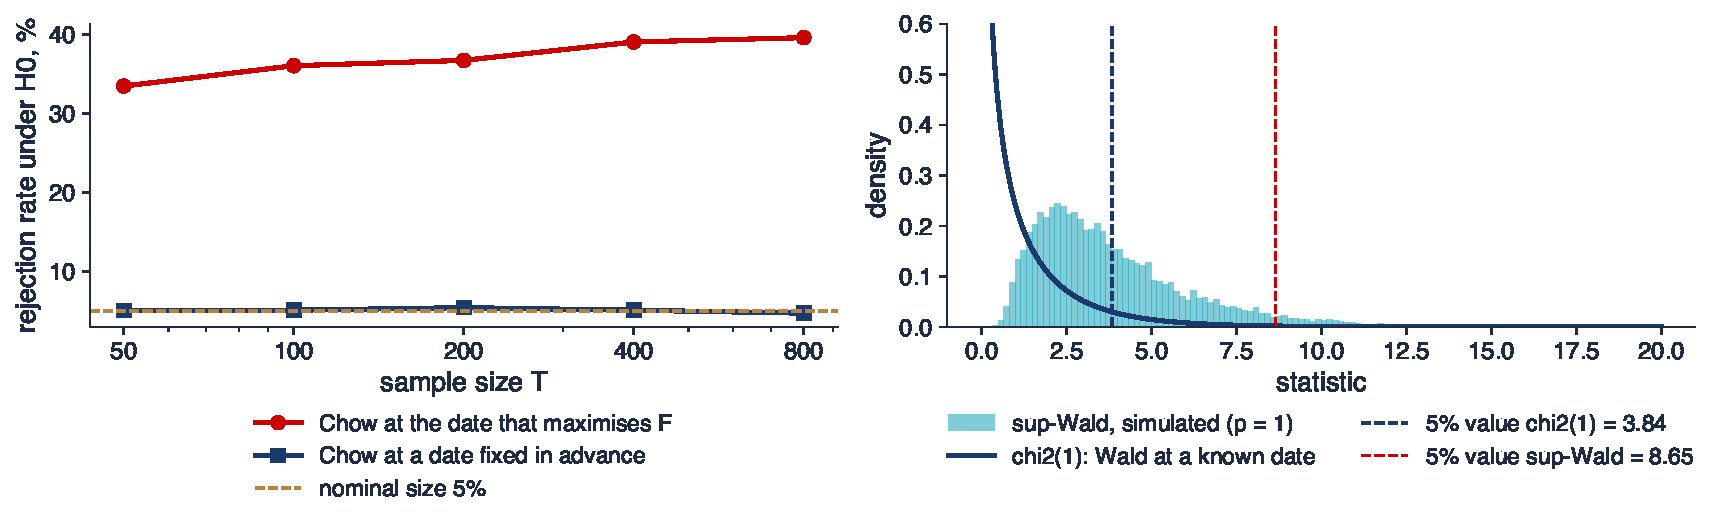
\includegraphics[width=0.97\textwidth,height=0.52\textheight,keepaspectratio]{ats_ch2_chow_snooping.pdf}
\end{center}
\vspace{-0.25cm}
\begin{itemize}
    \item Left: white noise, mean-shift Chow test at 5\%, 4\,000 replications per $T$; right: simulated null density of $\sup_\pi W_T(\pi)$, $\pi \in [0.15, 0.85]$, against $\chi^2(1)$
\end{itemize}
\quantlet{ATS\_ch2\_chow\_snooping}{\qlurl{ATS_ch2_chow_snooping}}
\end{frame}

\begin{frame}{Interpreting the size distortion}
\itemsize{\small}
\begin{itemize}
    \item At a fixed date the test keeps its size (5.1\% for $T = 100$); at the maximising date it rejects a true null in 33\% to 40\% of samples
    \begin{itemize}
        \item the distortion grows slowly with $T$: more candidate dates, a larger maximum
    \end{itemize}
    \item The 5\% critical value of the supremum is 8.65, against 3.84 for $\chi^2(1)$; with two coefficients 11.69
    \item Lesson: the date search is part of the test; the critical values must account for it
\end{itemize}
\end{frame}

\begin{frame}{Recap: Instability and known dates}
\itemsize{\small}
\begin{itemize}
    \item A break is a change of $\beta_t$; pure or partial, in mean, dynamics or variance
    \item Chow: an $F$ test valid only for a date fixed before seeing the data
    \item Choosing the date from the data multiplies the size several times
    \item The break date is a nuisance parameter not identified under $H_0$
\end{itemize}
\end{frame}


%=============================================================================
\section{One break at an unknown date}
%=============================================================================

\begin{frame}{The sup-Wald test of Andrews (1993) (1/2)}
\itemsize{\small}
\begin{itemize}
    \item Compute the Chow--Wald statistic $W_T(\pi)$ at every candidate break fraction and take the largest \refAnd
    \begin{itemize}
        \item $\sup_{\pi \in \Pi} W_T(\pi)$, $\quad \Pi = [\pi_0, 1 - \pi_0]$
        \item $\Pi$: the candidate fractions; $\pi_0$: the \textbf{trimming}, usually 0.15, so that each regime has at least 15\% of the sample
        \item LM, Wald and LR versions share the same limit; \refQua\ used the LR version
    \end{itemize}
    \item \textbf{Theorem} \refAnd: under $H_0$ and regularity conditions (stationary, mixing regressors)
    \begin{itemize}
        \item $W_T(\cdot) \Rightarrow Q_p(\pi) = \dfrac{\|B_p(\pi) - \pi B_p(1)\|^2}{\pi(1 - \pi)}$
        \item $\Rightarrow$: convergence of the whole process in $\pi$; $B_p$: a $p$-dimensional standard Brownian motion; $p$: the number of coefficients allowed to break
        \item $B_p(\pi) - \pi B_p(1)$ is a Brownian bridge; $\pi(1 - \pi)$ is its variance: $Q_p(\pi)$ is a squared, standardised bridge (\atsapplink{atsapp1}{atssrc1}{Appendix})
    \end{itemize}
\end{itemize}
\end{frame}

\begin{frame}{The sup-Wald test of Andrews (1993) (2/2)}
\itemsize{\small}
\begin{itemize}
    \item Limit: $\sup W_T \to_d \sup_{\pi \in \Pi} Q_p(\pi)$
    \begin{itemize}
        \item at a fixed $\pi$, $Q_p(\pi) \sim \chi^2(p)$; the supremum over many $\pi$ is much larger
    \end{itemize}
    \item Why trimming: $\sup_{\pi \in (0,1)} Q_p(\pi) = \infty$ almost surely (law of the iterated logarithm)
    \begin{itemize}
        \item critical values depend on $p$ and $\pi_0$; here simulated: $p = 1$: 7.11 (10\%), 8.65 (5\%), 12.17 (1\%)
    \end{itemize}
\end{itemize}
\end{frame}

\begin{frame}{Optimal tests: Andrews and Ploberger (1994)}
\itemsize{\small}
\begin{itemize}
    \item The supremum is not the only functional; averaging is optimal against alternatives close to $H_0$ \refAP
    \begin{itemize}
        \item $|\Pi| = 1 - 2\pi_0$: the length of the set of candidate fractions; both statistics average over it
        \item $\mathrm{expW} = \ln\Big(\dfrac{1}{|\Pi|}\displaystyle\int_\Pi \exp\big(\tfrac12 W_T(\pi)\big)d\pi\Big)$: weighted average power, for medium and large breaks
        \item $\mathrm{aveW} = \dfrac{1}{|\Pi|}\displaystyle\int_\Pi W_T(\pi)\,d\pi$: optimal for very small breaks, close to the Nyblom test of random-walk coefficients
    \end{itemize}
    \item 5\% values for $p = 1$, $\pi_0 = 0.15$ (simulated): sup 8.65, exp 2.02, ave 2.87
    \item The sup-Wald test has power against \emph{any} kind of instability, not only a single break
    \begin{itemize}
        \item a rejection says ``unstable'', not ``one break at $\hat\pi$''; the number of breaks is the subject of Section 3
    \end{itemize}
\end{itemize}
\end{frame}

\begin{frame}{Estimating the break date (1/2)}
\itemsize{\small}
\begin{itemize}
    \item Least squares: choose the date that minimises the total SSR of the two regimes
    \begin{itemize}
        \item $\hat T_1 = \arg\min_{T_1} [S_1(T_1) + S_2(T_1)]$
        \item $S_1(T_1)$, $S_2(T_1)$: the SSR before and after a candidate date $T_1$; equivalently the date of the largest Wald statistic under homoskedasticity
    \end{itemize}
    \item Precision \refBai
    \begin{itemize}
        \item for a fixed break size, $\hat T_1 - T_1 = O_p(1)$: the \textbf{date} error is bounded in probability and does not grow with $T$
        \item so the fraction $\hat\pi = \hat T_1/T$ converges at rate $T$, faster than the usual $\sqrt T$
        \item the regime coefficients are $\sqrt T$-consistent and asymptotically Normal as if the date were known
    \end{itemize}
\end{itemize}
\end{frame}

\begin{frame}{Estimating the break date (2/2)}
\itemsize{\small}
\begin{itemize}
    \item Confidence interval for the date \refBai: with a shrinking break $\Delta_T \to 0$
    \begin{itemize}
        \item $\Delta_T^2\sigma^{-2}(\hat T_1 - T_1) \to_d \arg\max_s Z(s)$, $\quad Z(s) = W(s) - |s|/2$
        \item $\Delta_T$: the size of the change in the mean; $\sigma^2$: the error variance; $W(s)$: a two-sided Brownian motion, $s \in \mathbb R$
        \item the interval is the date $\pm$ quantiles of $\arg\max Z$, rescaled by $\sigma^2/\hat\Delta^2$
    \end{itemize}
    \item Reading
    \begin{itemize}
        \item large breaks, small noise: a short interval; the interval is asymmetric when variances differ across regimes
    \end{itemize}
\end{itemize}
\end{frame}

\begin{frame}{Case study: McConnell and Perez-Quiros (2000)}
\itemsize{\footnotesize}
\begin{columns}[T]
\begin{column}{0.36\textwidth}
\centering
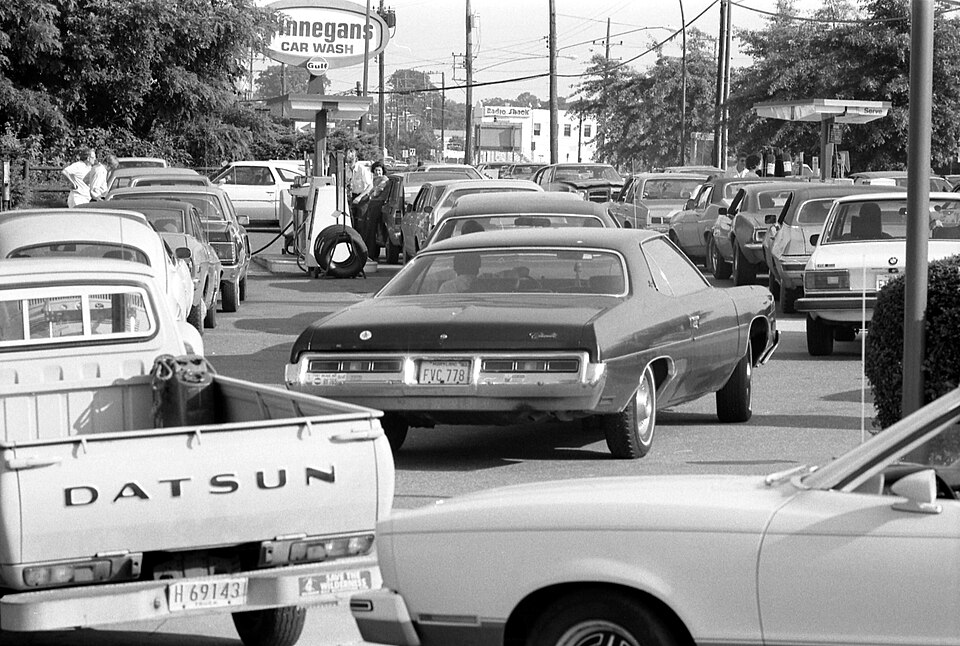
\includegraphics[height=0.36\textheight]{ch2_gasline_1979.jpg}\\[1mm]
\imgcap{Gasoline queue, Maryland, 15 June 1979}
\imgcredit{https://commons.wikimedia.org/wiki/File:Line_at_a_gas_station,_June_15,_1979.jpg}{Photo: Warren K. Leffler (1979), Library of Congress; public domain; Wikimedia Commons}
\end{column}
\begin{column}{0.62\textwidth}
\begin{itemize}
    \item The paper: US real GDP growth, 1953Q2--1999Q2; AR(1) for the conditional mean; then a break in the mean of $\sqrt{\pi/2}\,|\hat e_t|$, an unbiased estimate of the standard deviation under Normality \refMPQ
    \begin{itemize}
        \item $\hat e_t$: the AR(1) residual; here $\pi = 3.14\ldots$; if $e_t \sim N(0, \sigma^2)$, $\E|e_t| = \sigma\sqrt{2/\pi}$, hence the factor
        \item tests: sup-, exp-, ave-Wald \refAnd, \refAP; their result: a variance break in 1984Q1, the ``Great Moderation''
    \end{itemize}
    \item Our replication: the same two steps on FRED GDPC1 (today's vintage), robust Wald statistics, simulated $p$-values; then the sample extended to 2026
    \item Question: does the variance break survive revised data and the COVID-19 quarters?
\end{itemize}
\end{column}
\end{columns}
\end{frame}

\begin{frame}{The Great Moderation in US output growth}
\itemsize{\footnotesize}
\begin{center}
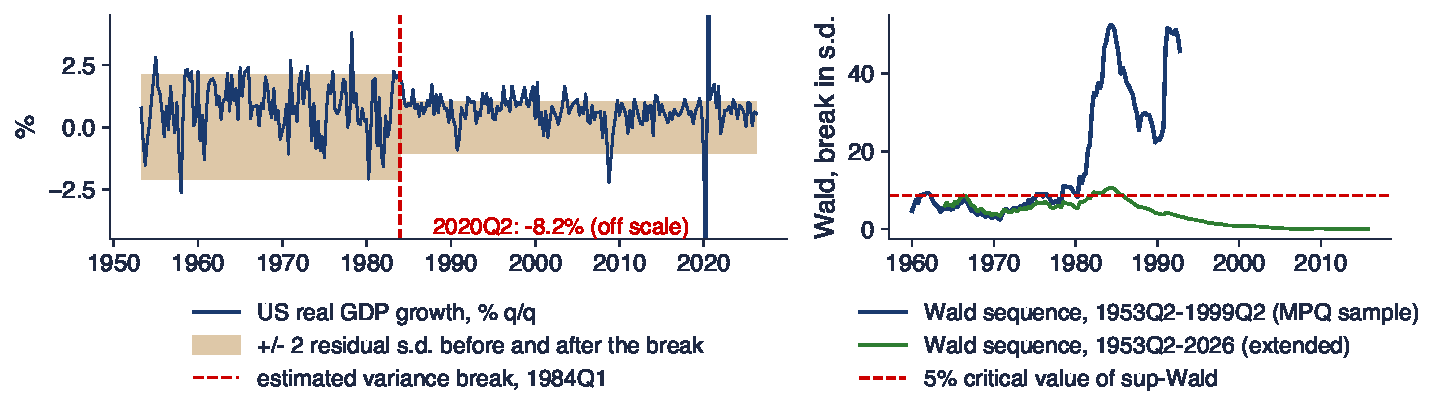
\includegraphics[width=0.97\textwidth,height=0.64\textheight,keepaspectratio]{ats_ch2_great_moderation.pdf}
\end{center}
\vspace{-0.25cm}
\begin{itemize}
    \item Top: growth with $\pm 2$ residual standard deviations before and after the estimated break; bottom: the Wald sequence for a break in $\E\sqrt{\pi/2}|e_t|$ (HAC), two samples
\end{itemize}
\quantlet{ATS\_ch2\_great\_moderation}{\qlurl{ATS_ch2_great_moderation}}
\end{frame}

\begin{frame}{Interpreting the variance break}
\itemsize{\small}
\begin{itemize}
    \item MPQ sample ($T = 185$): sup-Wald 52.5 ($p$ $<$\,0.001), exp 23.2, ave 17.5; date 1984Q1, the date found by \refMPQ
    \begin{itemize}
        \item residual s.d. 1.06 before, 0.45 after: the variance falls by a factor of 5.5; no break in the mean equation (sup 3.2, $p$ 0.861)
    \end{itemize}
    \item To 2019: the break moves by one quarter (1984Q2), variance ratio 4.1; the Great Moderation survived the 2008--2009 recession
    \item To 2026: sup-Wald falls to 10.7 ($p$ 0.019) and the ratio to 1.1: two outliers (2020Q2: \ensuremath{-}8.2\%) dominate the post-break variance
    \begin{itemize}
        \item a second break, or outliers? A one-break test cannot say; robust scale estimators or a second break are needed
    \end{itemize}
\end{itemize}
\end{frame}

\begin{frame}{Recap: One break at an unknown date}
\itemsize{\small}
\begin{itemize}
    \item sup-Wald: the supremum of a squared Brownian bridge; trim, and use its own critical values
    \item exp- and ave-Wald are optimal for moderate and small breaks
    \item The date is estimated precisely, the CI comes from $\arg\max_s\{W(s) - |s|/2\}$
    \item Variance breaks: test the mean of $|\hat e_t|$; outliers can mask or mimic them
\end{itemize}
\end{frame}


%=============================================================================
\section{Multiple breaks: Bai and Perron}
%=============================================================================

\begin{frame}{The multiple-break model}
\itemsize{\small}
\begin{itemize}
    \item $y_t = x_t'\beta + z_t'\delta_j + u_t$, $t = T_{j-1} + 1, \dots, T_j$, $j = 1, \dots, m + 1$, with $T_0 = 0$, $T_{m+1} = T$ \refBPa
    \begin{itemize}
        \item $T_1 < \dots < T_m$: the break dates; $\delta_j$: the coefficients of $z_t$ in regime $j$; $\beta$: those of $x_t$, common to all regimes
        \item pure change: no $x_t$; mean-shift model: $z_t = 1$
        \item minimum segment length $h = [\varepsilon T]$, usually $\varepsilon = 0.15$; errors may be autocorrelated and heteroskedastic across regimes
    \end{itemize}
    \item Estimator: the \textbf{global} minimiser of the SSR over all admissible partitions $(T_1, \dots, T_m)$
    \begin{itemize}
        \item break fractions consistent at rate $T$, as for one break; the dates are estimated jointly, not one at a time
    \end{itemize}
    \item Brute force needs $O(T^m)$ regressions; dynamic programming needs $O(T^2)$ \refBPb
\end{itemize}
\end{frame}

\begin{frame}{Dynamic programming}
\itemsize{\small}
\begin{itemize}
    \item Step 1: compute $\mathrm{SSR}(i, j)$ of one regression on every segment $[i, j]$ with $j - i + 1 \ge h$ (recursive residuals: $O(T^2)$ operations)
    \item Step 2: Bellman recursion for the best $r$-break partition of the first $n$ observations
    \begin{itemize}
        \item $\mathrm{SSR}(\{T_{r,n}\}) = \min_{rh \le j \le n - h}\big[\mathrm{SSR}(\{T_{r-1,j}\}) + \mathrm{SSR}(j + 1, n)\big]$
        \item $\{T_{r,n}\}$: the best partition of observations $1, \dots, n$ with $r$ breaks; $j$: the date of its last break; $h$: the minimum segment length
        \item the optimal $m$-break partition contains optimal partitions of its prefixes (Bellman's principle)
    \end{itemize}
    \item One pass gives the optimal partitions for every $m \le M$: the input of all tests and criteria
    \begin{itemize}
        \item partial change ($\beta$ common) needs an iteration between $\beta$ and the partition \refBPb; Seminar 2, A3 runs the recursion by hand
    \end{itemize}
\end{itemize}
\end{frame}

\begin{frame}{Testing and selecting the number of breaks (1/2)}
\itemsize{\small}
\begin{itemize}
    \item $\sup F_T(k)$: no break against exactly $k$ breaks, at the SSR-optimal partition, with robust variance \refBPa
    \begin{itemize}
        \item $M$: the largest number of breaks considered (here 5)
        \item \textbf{UDmax} $= \max_{k \le M}\sup F_T(k)$: no break against an unknown number of breaks, up to $M$
        \item \textbf{WDmax}: the same, with each $k$ weighted by the ratio of critical values
    \end{itemize}
    \item \textbf{Sequential} $\sup F_T(\ell + 1 \mid \ell)$: $\ell$ breaks against $\ell + 1$
    \begin{itemize}
        \item for each of the $\ell + 1$ segments, the largest single-break statistic; add a break while it rejects
        \item recommended strategy \refBPb: UDmax or WDmax first, then the sequential tests
    \end{itemize}
\end{itemize}
\end{frame}

\begin{frame}{Testing and selecting the number of breaks (2/2)}
\itemsize{\small}
\begin{itemize}
    \item Information criteria: pick the $m$ with the smallest value
    \begin{itemize}
        \item $\mathrm{BIC}(m) = \ln(\mathrm{SSR}_m/T) + p^*\ln T/T$
        \item \textbf{LWZ}: $\ln\frac{\mathrm{SSR}_m}{T - p^*} + p^*\frac{0.299}{T}(\ln T)^{2.1}$ \refLWZ
        \item $\mathrm{SSR}_m$: the SSR of the best $m$-break partition; $p^*$: the number of coefficients and break dates; the second term penalises extra breaks
    \end{itemize}
    \item Known weaknesses
    \begin{itemize}
        \item BIC picks too many breaks under serial correlation, LWZ too few with small breaks
    \end{itemize}
\end{itemize}
\end{frame}

\begin{frame}{Case study: Bai and Perron (2003), the US real interest rate}
\itemsize{\footnotesize}
\begin{columns}[T]
\begin{column}{0.36\textwidth}
\centering
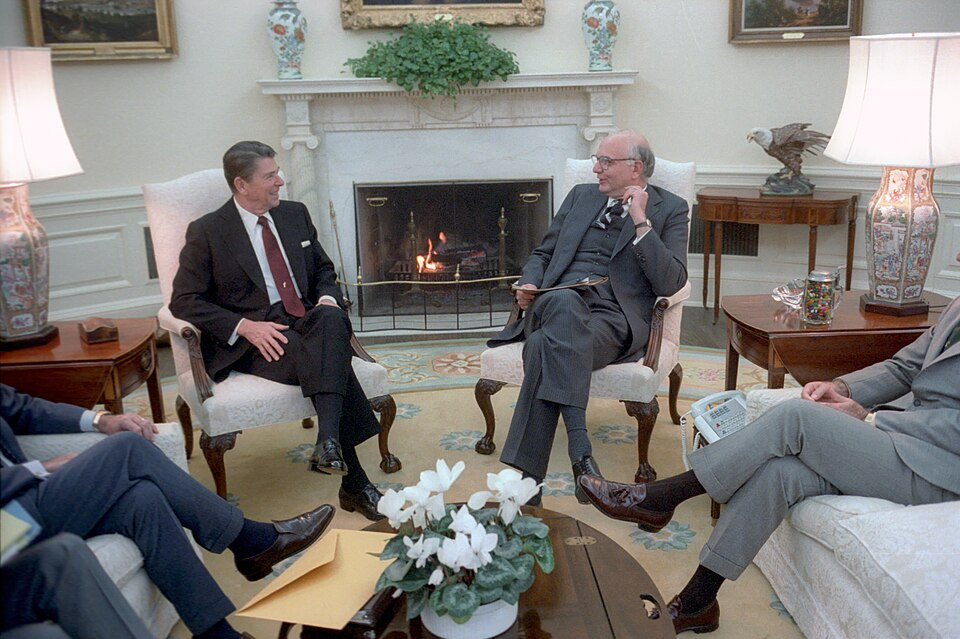
\includegraphics[height=0.33\textheight]{ch2_volcker_reagan_1981.jpg}\\[1mm]
\imgcap{Paul Volcker (left) and Ronald Reagan, December 1981}
\imgcredit{https://commons.wikimedia.org/wiki/File:President_Ronald_Reagan_Paul_Volcker_Meeting_to_Discuss_Monetary_Policy_with_Paul_Volker_in_Oval_Office_-_DPLA_-_e04117f4897610a724c267cdf855ce73.jpg}{Photo: White House Photographic Office (1981); public domain; Wikimedia Commons}
\end{column}
\begin{column}{0.62\textwidth}
\begin{itemize}
    \item The paper, Section 6.1: the ex-post real rate of \refGP, quarterly 1961Q1--1986Q3 ($T = 103$), mean-shift model, $\varepsilon = 0.15$ ($h = 15$), $M = 5$, HAC variances that differ across segments \refBPb
    \begin{itemize}
        \item our replication uses their data file (JAE data archive) and the same settings
    \end{itemize}
    \item Extension: the series rebuilt from FRED (T-bill rate at the end of the quarter minus next-quarter CPI inflation), correlation 0.99 with the original, 1961Q1--2026Q1
    \item Question: how many regimes, and do they match the history of monetary policy?
\end{itemize}
\end{column}
\end{columns}
\end{frame}

\begin{frame}{Mean shifts in the US real interest rate}
\itemsize{\footnotesize}
\begin{center}
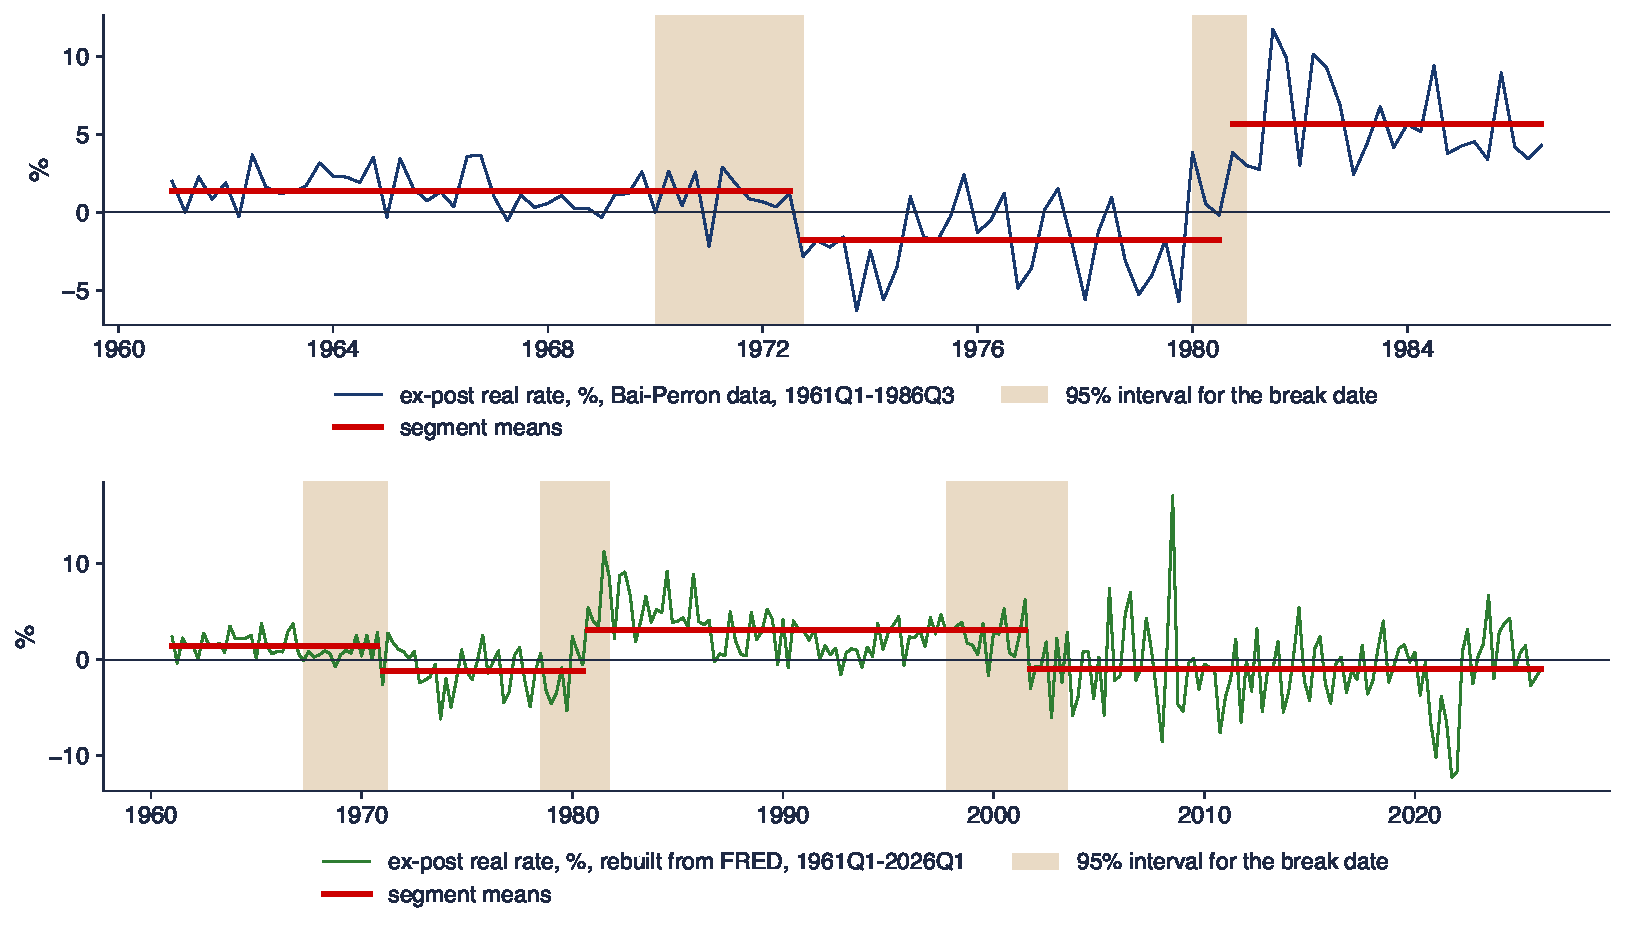
\includegraphics[width=0.97\textwidth,height=0.64\textheight,keepaspectratio]{ats_ch2_bai_perron.pdf}
\end{center}
\vspace{-0.25cm}
\begin{itemize}
    \item Red: segment means of the BIC/LWZ partition; shaded: 95\% intervals for the dates \refBai, heterogeneous long-run variances. Top: original data; bottom: rebuilt to 2026
\end{itemize}
\quantlet{ATS\_ch2\_bai\_perron}{\qlurl{ATS_ch2_bai_perron}}
\end{frame}

\begin{frame}{Interpreting the Bai--Perron results}
\itemsize{\footnotesize}
\begin{center}
\scriptsize
\begin{tabular}{lrrrrrr}
\toprule
\textbf{$m$} & 0 & 1 & 2 & 3 & 4 & 5 \\
\midrule
SSR & 1215 & 645 & 456 & 445 & -- & -- \\
$\sup F_T(m)$ & -- & 61.1 & 46.1 & 36.1 & 27.4 & 20.6 \\
5\% value & -- & 8.74 & 7.27 & 6.05 & -- & -- \\
BIC & 2.513 & 1.970 & 1.713 & 1.779 & -- & -- \\
LWZ & 2.550 & 2.082 & 1.901 & 2.043 & -- & -- \\
\bottomrule
\end{tabular}
\end{center}
\begin{itemize}
    \item UDmax 61.1 (5\%: 8.87); sequential: $F(2|1) = 36.9$, $F(3|2) = 16.1$, $F(4|3) = 0.04$ (5\%: 10.54, 11.56): 3 breaks, 1966Q4, 1972Q3, 1980Q3
    \begin{itemize}
        \item BIC and LWZ choose 2 breaks: 1972Q3, 1980Q3; the dates are the ones reported by \refBPb
    \end{itemize}
    \item Means 1.36\%, \ensuremath{-}1.80\%, 5.64\%: negative real rates in the 1970s, then the 1979--1981 disinflation; 95\% intervals [1970Q1, 1972Q4], [1980Q1, 1981Q1]
    \item Extended sample: 3 breaks (1970Q4, 1980Q3, 2001Q3); the last regime has a mean of \ensuremath{-}0.97\%: the low-rate era after 2001, interval [1997Q4, 2003Q3]
\end{itemize}
\end{frame}

\begin{frame}{Mean shifts in Romanian inflation}
\itemsize{\footnotesize}
\begin{center}
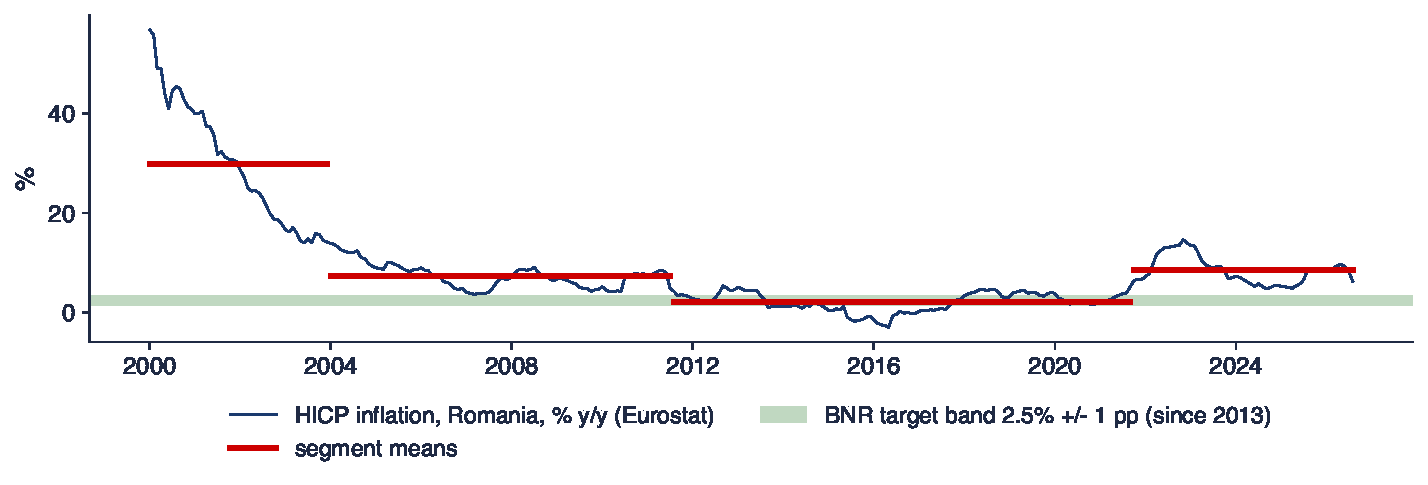
\includegraphics[width=0.97\textwidth,height=0.48\textheight,keepaspectratio]{ats_ch2_ro_inflation_breaks.pdf}
\end{center}
\vspace{-0.25cm}
\begin{itemize}
    \item HICP inflation, y/y, January 2000--August 2026 ($T = 320$), Bai--Perron mean shifts, $\varepsilon = 0.15$, $M = 5$; red: the partition chosen by BIC and LWZ
\end{itemize}
\quantlet{ATS\_ch2\_ro\_inflation\_breaks}{\qlurl{ATS_ch2_ro_inflation_breaks}}
\end{frame}

\begin{frame}{Interpreting the Romanian inflation regimes}
\itemsize{\small}
\begin{itemize}
    \item BIC and LWZ: 3 breaks (December 2003, July 2011, September 2021); means 29.8\%, 7.5\%, 2.2\%, 8.5\%
    \begin{itemize}
        \item disinflation, inflation targeting (adopted in August 2005), the low-inflation decade, the 2021--2023 surge
    \end{itemize}
    \item The robust sequential procedure stops at 1 break: $\sup F(1) = 12.8$, but $F(2|1) = 2.06$
    \begin{itemize}
        \item inflation is very persistent within regimes: the HAC variance absorbs the shifts, and the test loses power
        \item for the same reason the 95\% intervals for the dates span years (second date: [January 2000, December 2014]); they are not drawn
    \end{itemize}
    \item Better model: partial change in the intercept of an AR model, so that the errors are close to white noise (project idea)
\end{itemize}
\end{frame}

\begin{frame}{Change-point detection in statistics and machine learning}
\itemsize{\small}
\begin{itemize}
    \item Penalised segmentation: minimise $\sum_j \mathrm{cost}(\text{segment } j) + \beta\,m$ over partitions
    \begin{itemize}
        \item $\mathrm{cost}$: e.g.\ the SSR or minus the log-likelihood of a segment; $\beta > 0$: the penalty per break; $m$: the number of breaks
        \item PELT prunes the Bellman recursion to $O(T)$ under mild conditions \refKFE; binary segmentation and wild binary segmentation \refFry\ scale to long series
        \item the Python package \texttt{ruptures} implements them \refTOV; the BIC of Bai--Perron is a particular penalty
    \end{itemize}
    \item What econometrics adds: inference on the number of breaks and confidence intervals for dates under serial correlation
    \begin{itemize}
        \item common breaks in systems of equations \refOP; survey \refCP
    \end{itemize}
    \item Engineering practice tunes the penalty on labelled data; econometrics fixes the size of a test: both are valid if the choice is pre-registered
\end{itemize}
\end{frame}

\begin{frame}{Recap: Multiple breaks}
\itemsize{\small}
\begin{itemize}
    \item Global least squares over all partitions, by dynamic programming in $O(T^2)$
    \item UDmax/WDmax, then sequential $F(\ell + 1|\ell)$; BIC and LWZ as a cross-check
    \item US real rate: breaks in 1972Q3 and 1980Q3 replicated; a further regime after 2001
    \item Persistent errors: robust tests lose power and date intervals become wide
\end{itemize}
\end{frame}


%=============================================================================
\section{Fluctuation tests and real-time monitoring}
%=============================================================================

\begin{frame}{CUSUM and MOSUM tests (1/2)}
\itemsize{\small}
\begin{itemize}
    \item Recursive residuals \refBDE: the standardised one-step forecast error of the model estimated up to $t - 1$
    \begin{itemize}
        \item $w_t = (y_t - x_t'\hat\beta_{t-1})/\sqrt{1 + x_t'(X_{t-1}'X_{t-1})^{-1}x_t}$
        \item $\hat\beta_{t-1}$: OLS on observations $1, \dots, t - 1$; $X_{t-1}$: the matrix of their regressors; the root rescales for estimation uncertainty
        \item under $H_0$ with Normal errors, $w_t$ are i.i.d.\ $N(0, \sigma^2)$
    \end{itemize}
    \item CUSUM: the cumulated standardised recursive residuals
    \begin{itemize}
        \item $W_r = \hat\sigma^{-1}\sum_{t = k+1}^{r} w_t$, 5\% boundary $\pm 0.948[\sqrt{T - k} + 2(r - k)/\sqrt{T - k}]$
        \item $k$: the number of regressors (the first $k$ observations start the recursion); $W_r$ behaves like a Brownian motion; a crossing signals a break
    \end{itemize}
\end{itemize}
\end{frame}

\begin{frame}{CUSUM and MOSUM tests (2/2)}
\itemsize{\small}
\begin{itemize}
    \item What CUSUM detects
    \begin{itemize}
        \item changes in the intercept and a systematic drift of forecast errors; weak against changes that average out
    \end{itemize}
    \item OLS-CUSUM uses ordinary residuals: a Brownian bridge limit \refPK; MOSUM sums over a moving window of fixed width \refCHK
    \begin{itemize}
        \item MOSUM reacts faster to a break in the middle of the sample and to temporary changes
    \end{itemize}
    \item These are \textbf{retrospective} tests: the whole sample is available when the test is run
\end{itemize}
\end{frame}

\begin{frame}{Monitoring: the failure of repeated tests (1/2)}
\itemsize{\small}
\begin{itemize}
    \item A central bank estimates a model on $m$ historical observations and asks, at every new release, ``has it broken down?''
    \begin{itemize}
        \item a 5\% test repeated at $n = m + 1, m + 2, \dots$ rejects a true $H_0$ eventually with probability 1: the law of the iterated logarithm
    \end{itemize}
    \item \refCSW: monitor the CUSUM of the new recursive residuals and stop the first time it crosses a widening boundary
    \begin{itemize}
        \item $Q_n = \hat\sigma^{-1}\sum_{t = m+1}^{n} w_t$, $\quad$ alarm if $|Q_n| > \sqrt{n\,[a^2 + \ln(n/m)]}$
        \item $n$: the current sample size; $a$: a constant chosen to fix the false-alarm probability; the $\ln(n/m)$ term widens the boundary as time passes
    \end{itemize}
\end{itemize}
\end{frame}

\begin{frame}{Monitoring: the failure of repeated tests (2/2)}
\itemsize{\small}
\begin{itemize}
    \item The boundary comes from \refRS:
    \begin{itemize}
        \item $P\{\exists u \ge 1: |W(u) - W(1)| \ge \sqrt{u(a^2 + \ln u)}\} = 2[1 - \Phi(a) + a\varphi(a)]$
        \item $W$: a standard Brownian motion; $u = n/m$; $\Phi$, $\varphi$: the standard Normal distribution and density functions
        \item $a^2 = 7.78$: size 5.1\% over an \emph{infinite} horizon; $a^2 = 6.25$: 10.0\%
    \end{itemize}
    \item Forecast-based monitoring: forecast breakdowns \refGRa\ and the fluctuation test of relative accuracy \refGRb\ (\atschlink{https://danpele.github.io/Advanced-Time-Series/EN/Courses/chapter1_forecast_evaluation.pdf}{Chapter 1})
\end{itemize}
\end{frame}

\begin{frame}{False alarms and real-time monitoring of Romanian inflation}
\itemsize{\footnotesize}
\begin{center}
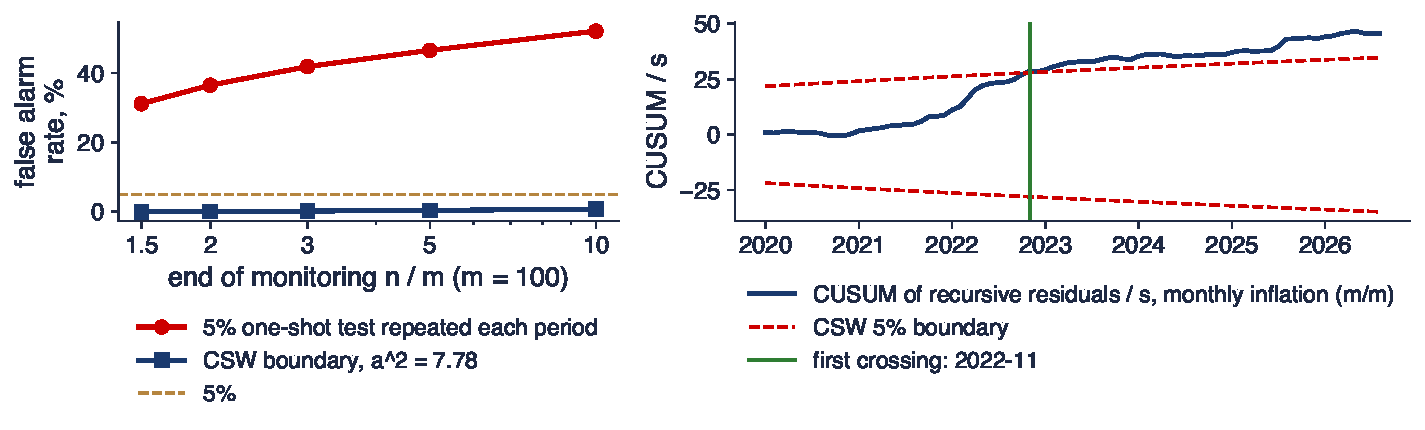
\includegraphics[width=0.97\textwidth,height=0.5\textheight,keepaspectratio]{ats_ch2_monitoring.pdf}
\end{center}
\vspace{-0.25cm}
\begin{itemize}
    \item Left: white noise, $m = 100$, 2\,000 replications; right: mean of monthly HICP inflation (m/m), historical sample 2015--2019, monitoring from January 2020
\end{itemize}
\quantlet{ATS\_ch2\_monitoring}{\qlurl{ATS_ch2_monitoring}}
\end{frame}

\begin{frame}{Interpreting the monitoring results}
\itemsize{\small}
\begin{itemize}
    \item Repeated 5\% tests raise a false alarm in 36\% of samples by $n = 2m$ and in 52\% by $n = 10m$; the CSW boundary in 0.8\%
    \begin{itemize}
        \item the CSW size is reached only as $n \to \infty$: over a finite horizon the boundary is conservative
    \end{itemize}
    \item Romania: historical mean 0.15\% per month, $\hat\sigma = 0.51$; the CUSUM crosses the boundary in November 2022
    \begin{itemize}
        \item the repeated naive test would have signalled in January 2022; with a long-run $\hat\sigma$ (HAC) the signal comes only in August 2025
    \end{itemize}
    \item The price of a controlled false-alarm rate is delay: nearly two years after inflation started to rise in 2021
\end{itemize}
\end{frame}

\begin{frame}{Recap: Monitoring}
\itemsize{\small}
\begin{itemize}
    \item CUSUM and MOSUM of recursive residuals: retrospective fluctuation tests
    \item Repeating a one-shot test as data arrive guarantees a false alarm
    \item CSW boundary $\sqrt{n[a^2 + \ln(n/m)]}$ controls the size over an infinite horizon
    \item Romanian inflation: detection in late 2022, a long but honest delay
\end{itemize}
\end{frame}


%=============================================================================
\section{Breaks in variance}
%=============================================================================

\begin{frame}{The ICSS algorithm and its correction (1/2)}
\itemsize{\small}
\begin{itemize}
    \item \refIT: compare the cumulated sum of squares with a straight line
    \begin{itemize}
        \item $C_k = \sum_{t \le k} a_t^2$, $\quad D_k = C_k/C_T - k/T$, $\quad \mathrm{IT} = \sqrt{T/2}\max_k|D_k| \Rightarrow \sup|B^0(r)|$
        \item $a_t$: the demeaned returns; $C_k/C_T$: the share of the total sum of squares reached at $k$; with a constant variance it grows like $k/T$
        \item $B^0$: a Brownian bridge on $[0,1]$; 5\% critical value 1.358; the date is the $k$ of the largest $|D_k|$
    \end{itemize}
    \item ICSS (iterated cumulative sums of squares)
    \begin{itemize}
        \item apply the test iteratively to sub-segments (binary segmentation), then re-check each break between its neighbours
    \end{itemize}
\end{itemize}
\end{frame}

\begin{frame}{The ICSS algorithm and its correction (2/2)}
\itemsize{\small}
\begin{itemize}
    \item The factor $\sqrt{T/2}$ assumes $\Var(a_t^2) = 2\sigma^4$: i.i.d.\ Normal data
    \begin{itemize}
        \item with kurtosis $\kappa = \E a_t^4/\sigma^4$ the statistic is inflated by $\sqrt{(\kappa - 1)/2}$; with GARCH, $a_t^2$ is also autocorrelated
    \end{itemize}
    \item $\kappa_2$ of \refSAC: the same CUSUM, scaled by a long-run variance
    \begin{itemize}
        \item $\kappa_2 = \max_k|C_k - (k/T)C_T|/\sqrt{T\hat\omega_4}$
        \item $\hat\omega_4$: the long-run variance of $a_t^2 - \hat\sigma^2$ (Bartlett kernel, \atschlink{https://danpele.github.io/Advanced-Time-Series/EN/Courses/chapter0_refresher_inference.pdf}{Chapter 0})
        \item same limit, valid under fat tails and conditional heteroskedasticity
    \end{itemize}
\end{itemize}
\end{frame}

\begin{frame}{Variance regimes of EUR/RON}
\itemsize{\footnotesize}
\begin{center}
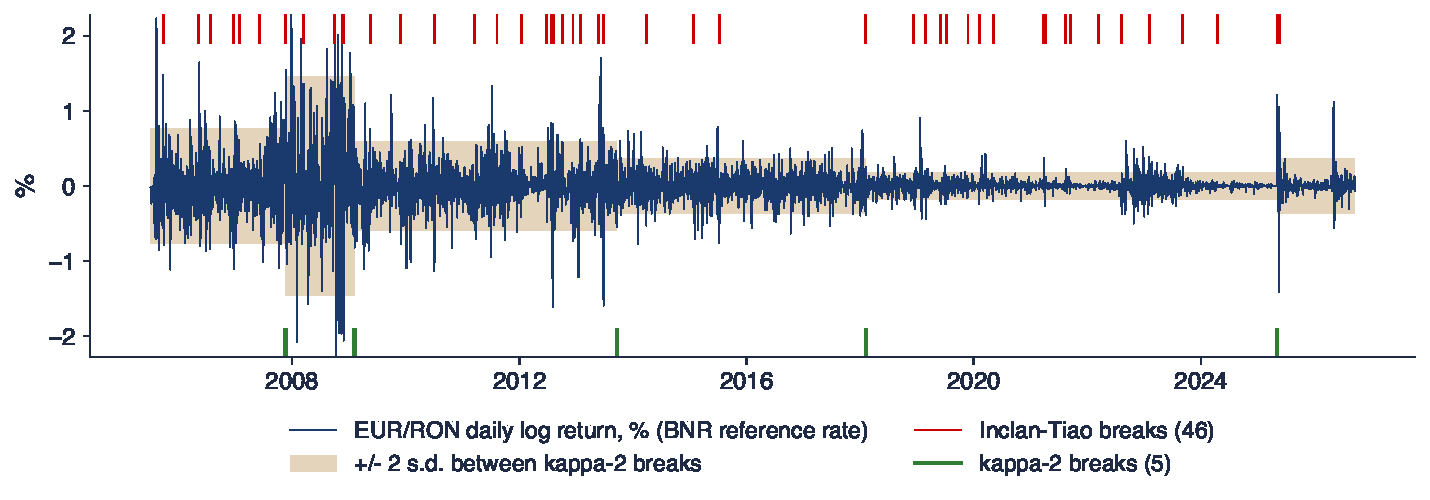
\includegraphics[width=0.97\textwidth,height=0.5\textheight,keepaspectratio]{ats_ch2_variance_breaks.pdf}
\end{center}
\vspace{-0.25cm}
\begin{itemize}
    \item Daily log returns of the BNR reference rate, 5\,352 days; red ticks: ICSS with the Inclán--Tiao statistic; green ticks and shaded bands: ICSS with $\kappa_2$
\end{itemize}
\quantlet{ATS\_ch2\_variance\_breaks}{\qlurl{ATS_ch2_variance_breaks}}
\end{frame}

\begin{frame}{Interpreting the EUR/RON variance breaks}
\itemsize{\small}
\begin{itemize}
    \item Excess kurtosis 15.1: the Inclán--Tiao statistic is 24.0 and ICSS finds 46 breaks; $\kappa_2 = 4.69$ and 5 breaks
    \begin{itemize}
        \item most Inclán--Tiao ``breaks'' are volatility clusters, not changes of the unconditional variance
    \end{itemize}
    \item $\kappa_2$ dates: 20 November 2007, 6 February 2009, 19 September 2013, 7 February 2018, 5 May 2025
    \begin{itemize}
        \item the global financial crisis, the end of its turbulence, the calmer managed float after 2018; daily s.d.\ between 0.09\% and 0.73\%
    \end{itemize}
    \item For risk models (\atschlink{https://danpele.github.io/MFM/EN/Courses/chapter5_garch_models.pdf}{MFM, Chapter 5}): a GARCH fitted across a variance break overstates persistence ($\alpha + \beta \to 1$) \refDI
\end{itemize}
\end{frame}


%=============================================================================
\section{Unit roots with breaks, revisited}
%=============================================================================

\begin{frame}{Beyond Zivot--Andrews}
\itemsize{\small}
\begin{itemize}
    \item \atschlink{https://danpele.github.io/Time-Series-Analysis/EN/Courses/chapter3_unit_roots_arima_models.pdf}{TSA, Chapter 3}: a level shift mimics a unit root \refPer; \refZA\ choose the date by minimising the ADF $t$ statistic
    \begin{itemize}
        \item their null is a unit root \emph{without} a break: a break under the null makes the test reject too often
    \end{itemize}
    \item Two breaks: \refLP\ minimise the $t$ statistic over two dates; \refLS\ propose an LM test whose null allows breaks
    \begin{itemize}
        \item \refKPe: pre-test the break, then use a test valid under both hypotheses
    \end{itemize}
    \item Critical values depend on the model, the trimming and the number of breaks; a sieve bootstrap under the null avoids the tables
\end{itemize}
\end{frame}

\begin{frame}{Romanian GDP: unit root or broken trend?}
\itemsize{\footnotesize}
\begin{center}
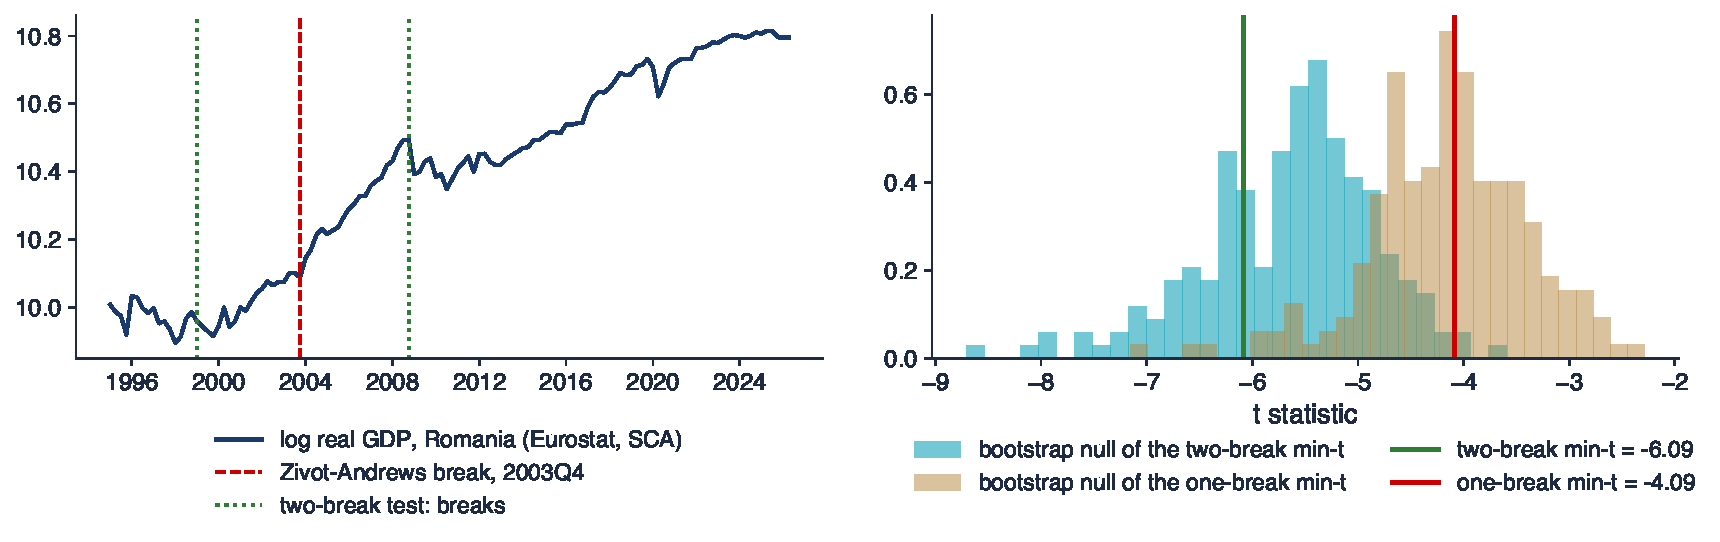
\includegraphics[width=0.97\textwidth,height=0.5\textheight,keepaspectratio]{ats_ch2_unit_root_breaks.pdf}
\end{center}
\vspace{-0.25cm}
\begin{itemize}
    \item Log real GDP (SCA), 1995Q1--2026Q2; one and two breaks in level and trend; null distributions from a sieve bootstrap (AR on $\Delta y_t$, 199 replications)
\end{itemize}
\quantlet{ATS\_ch2\_unit\_root\_breaks}{\qlurl{ATS_ch2_unit_root_breaks}}
\end{frame}

\begin{frame}{Interpreting the unit-root tests with breaks}
\itemsize{\small}
\begin{itemize}
    \item ADF with trend: \ensuremath{-}2.79 ($p$ 0.201); Zivot--Andrews: \ensuremath{-}4.09 at 2003Q4 (5\%: \ensuremath{-}5.07; bootstrap $p$ 0.523)
    \item Two breaks (1999Q1 and 2008Q4): min-$t$ = \ensuremath{-}6.09, bootstrap 5\% value \ensuremath{-}7.16, $p$ 0.266
    \begin{itemize}
        \item the more breaks we allow, the more negative the critical value: the apparent gain disappears
    \end{itemize}
    \item With about 30 years of quarterly data a unit root cannot be rejected; the convergence story (fast growth, then a 2009 break) remains a hypothesis
\end{itemize}
\end{frame}

\begin{frame}{Recap: Breaks in variance and unit roots}
\itemsize{\small}
\begin{itemize}
    \item ICSS needs the $\kappa_2$ correction for fat tails and GARCH
    \item EUR/RON: a handful of genuine variance regimes, not dozens
    \item Unit-root tests with breaks: allow breaks under the null or pre-test them; bootstrap the critical values
\end{itemize}
\end{frame}


%=============================================================================
\section{Forecasting under breaks}
%=============================================================================

\begin{frame}{Location shifts cause forecast failure}
\itemsize{\small}
\begin{itemize}
    \item \refCHa, \refCHb: in equilibrium-correction models, a shift of the equilibrium mean is the main source of systematic forecast errors
    \begin{itemize}
        \item after the shift, the model keeps pulling the forecast towards the old mean
    \end{itemize}
    \item Robust devices
    \begin{itemize}
        \item \textbf{intercept correction}: add the last observed error to the forecast
        \item \textbf{differencing}: forecast $\Delta y$; adapts after one period, at the cost of a larger variance
        \item \textbf{shorter windows}: rolling estimation, or the post-break sample
    \end{itemize}
    \item Survey of the evidence: \refRos; window choice with time-varying parameters \refIJR
\end{itemize}
\end{frame}

\begin{frame}{The choice of the estimation window}
\itemsize{\small}
\begin{itemize}
    \item Mean shift $\delta$ after $n_1$ pre-break observations, $n_2$ post-break; forecast with the last $w \ge n_2$ observations \refPT
    \begin{itemize}
        \item $\mathrm{MSFE}(w) = \sigma^2\big(1 + \tfrac1w\big) + \Big(\dfrac{(w - n_2)\delta}{w}\Big)^2$: variance falls with $w$, squared bias grows
        \item MSFE: the mean squared forecast error of the sample mean over the window; $\sigma^2$: the noise variance; $(w - n_2)/w$: the share of pre-break data in the window
        \item the optimal window includes \emph{some} pre-break data when $\delta/\sigma$ is small or $n_2$ short (Seminar 2, A8)
    \end{itemize}
    \item Feasible rules: estimate the date (Bai--Perron) and use the post-break sample; cross-validate $w$ \refPT; average forecasts across windows (AveW) \refPP
    \begin{itemize}
        \item the date is estimated with error exactly when the break is small: post-break windows are then too short
    \end{itemize}
\end{itemize}
\end{frame}

\begin{frame}{Window choice: simulation and Romanian inflation}
\itemsize{\footnotesize}
\begin{center}
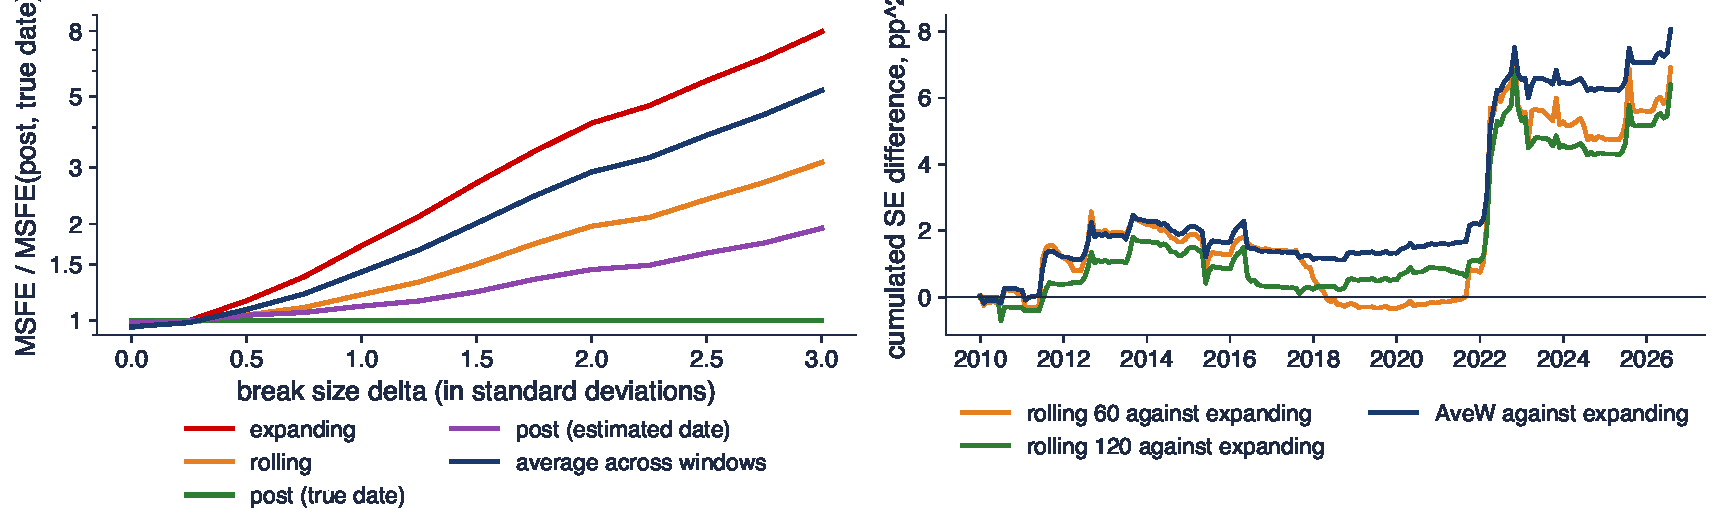
\includegraphics[width=0.97\textwidth,height=0.5\textheight,keepaspectratio]{ats_ch2_forecast_windows.pdf}
\end{center}
\vspace{-0.25cm}
\begin{itemize}
    \item Left: $T = 200$, break $n_2 = 20$ periods before the end, 4\,000 replications, MSFE relative to the post-break mean with the true date; right: AR(2), one month ahead, cumulated squared-error gains over the expanding window
\end{itemize}
\quantlet{ATS\_ch2\_forecast\_windows}{\qlurl{ATS_ch2_forecast_windows}}
\end{frame}

\begin{frame}{Interpreting the window choice}
\itemsize{\small}
\begin{itemize}
    \item Simulation: without a break the expanding window wins (0.95); with $\delta = 1$: expanding 1.71, rolling 1.21, AveW 1.42, estimated post-break 1.11
    \begin{itemize}
        \item $\delta = 2$: 4.13, 1.97, 2.91, 1.44: estimating the date pays when the break is large
    \end{itemize}
    \item Romania, $P = 200$ months: RMSE expanding 0.664, rolling 60: 0.638, rolling 120: 0.640, AveW 0.633 pp
    \begin{itemize}
        \item HLN against expanding: AveW 2.20 ($p$ 0.029), rolling 60 1.19 ($p$ 0.234); all gains arrive in 2022, the RMSE in 2021--2023 falls from 0.790 to 0.700
    \end{itemize}
    \item Averaging across windows is a cheap insurance: never far from the best window, without estimating any date
\end{itemize}
\end{frame}

\begin{frame}{Recap: Forecasting under breaks}
\itemsize{\small}
\begin{itemize}
    \item Location shifts drive forecast failure; intercept correction and differencing make forecasts robust
    \item Optimal window: a bias--variance trade-off that may include pre-break data
    \item AveW is robust when the break is uncertain; post-break windows when it is large and well dated
    \item Evaluate the window choice out of sample with DM--HLN \refDM, \refHLN\ (\atschlink{https://danpele.github.io/Advanced-Time-Series/EN/Courses/chapter1_forecast_evaluation.pdf}{Chapter 1})
\end{itemize}
\end{frame}


%=============================================================================
\section{Threshold autoregression}
%=============================================================================

\begin{frame}{Motivation for nonlinear models}
\itemsize{\footnotesize}
\begin{columns}[T]
\begin{column}{0.36\textwidth}
\centering
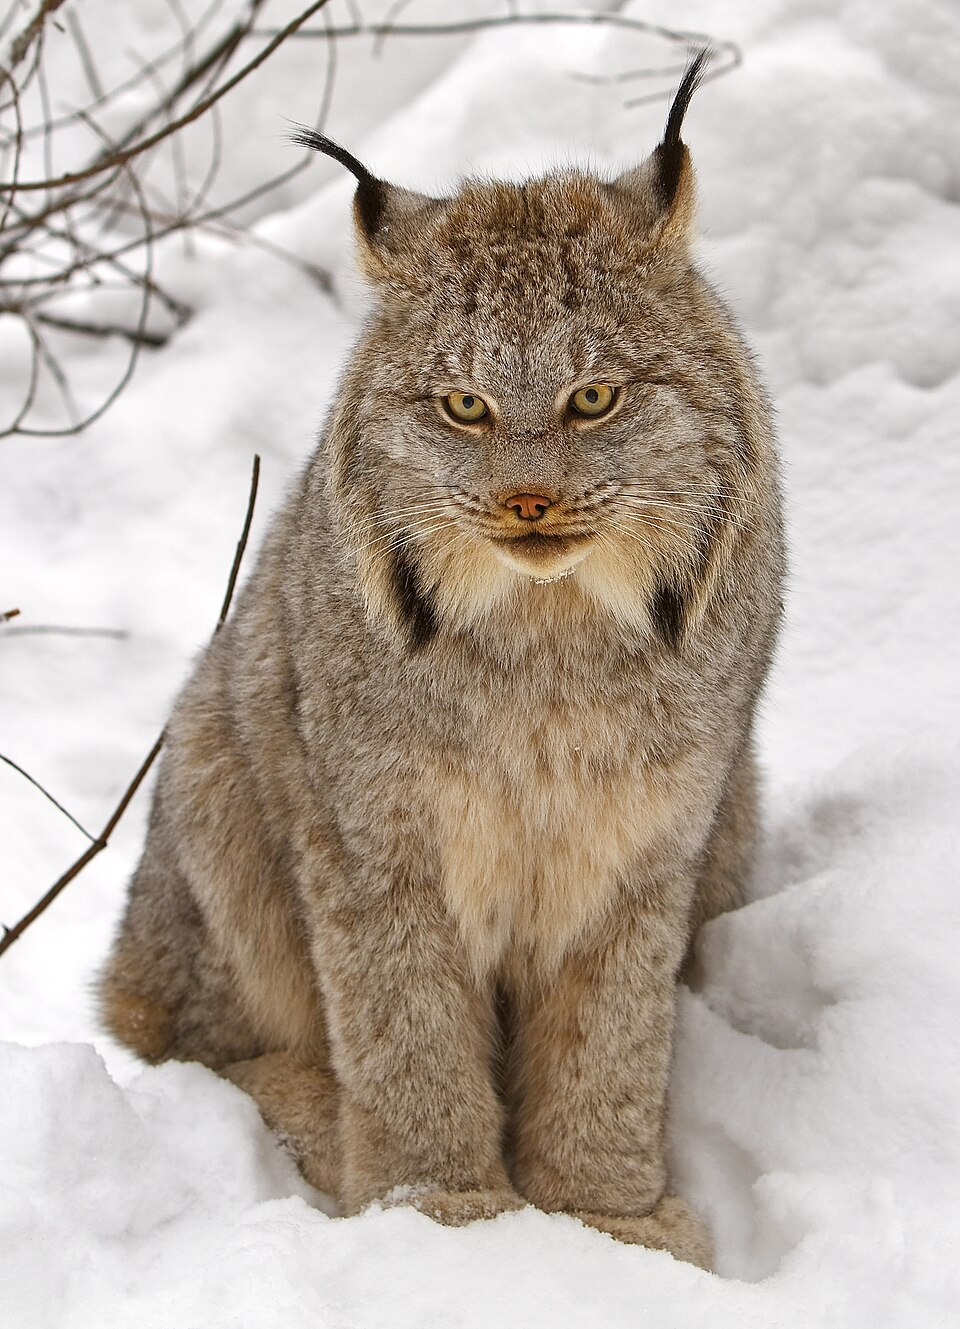
\includegraphics[height=0.36\textheight]{ch2_lynx_2010.jpg}\\[1mm]
\imgcap{Canada lynx}
\imgcredit{https://commons.wikimedia.org/wiki/File:Canada_lynx_by_Michael_Zahra_(cropped).jpg}{Photo: Michael Zahra (2010); CC BY-SA 3.0; Wikimedia Commons}
\end{column}
\begin{column}{0.62\textwidth}
\begin{itemize}
    \item Linear models are symmetric: a shock of $-1$ has the mirror effect of a shock of $+1$, at every state
    \begin{itemize}
        \item business cycles: unemployment rises fast in recessions and falls slowly in expansions \refNef
        \item arbitrage: real exchange rates move freely inside a band of transaction costs, revert outside it \refMNP
    \end{itemize}
    \item Ecology: the 9--10 year cycle of the Canadian lynx is asymmetric (slow rise, fast fall); a linear AR cannot produce a stable cycle without noise
    \item A nonlinear model can: limit cycles, asymmetry, state-dependent persistence and impulse responses
\end{itemize}
\end{column}
\end{columns}
\end{frame}

\begin{frame}{Threshold and self-exciting threshold autoregression (1/2)}
\itemsize{\small}
\begin{itemize}
    \item Two-regime \textbf{TAR}: an AR model whose coefficients depend on whether $q_{t-1}$ is below or above the threshold $\gamma$
    \begin{itemize}
        \item $y_t = (\phi_{1,0} + \phi_1'\mathbf y_{t-1})\mathbf 1\{q_{t-1} \le \gamma\} + (\phi_{2,0} + \phi_2'\mathbf y_{t-1})\mathbf 1\{q_{t-1} > \gamma\} + \varepsilon_t$
        \item $\mathbf y_{t-1} = (y_{t-1}, \dots, y_{t-p})'$: the last $p$ values; $\phi_{j,0}$, $\phi_j$: the intercept and AR coefficients of regime $j$
        \item $q_{t-1}$: the observed threshold variable; $\gamma$: the threshold; $\mathbf 1\{\cdot\}$ selects the regime; variances may differ across regimes
    \end{itemize}
    \item \textbf{SETAR} (self-exciting): $q_{t-1} = y_{t-d}$, the series itself with the \textbf{delay} lag $d$
    \begin{itemize}
        \item notation SETAR$(k; p_1, \dots, p_k)$: $k$ regimes with AR orders $p_1, \dots, p_k$ \refTL
    \end{itemize}
\end{itemize}
\end{frame}

\begin{frame}{Threshold and self-exciting threshold autoregression (2/2)}
\itemsize{\small}
\begin{itemize}
    \item Dynamics: the \textbf{skeleton} $y_t = F(\mathbf y_{t-1})$, the model with the noise switched off
    \begin{itemize}
        \item $F$: the regime-dependent conditional mean; the skeleton can converge to a point, a limit cycle or a chaotic attractor
    \end{itemize}
    \item Stationarity is a property of the whole model, not of each regime
    \begin{itemize}
        \item SETAR(2; 1, 1) is ergodic iff $\phi_1 < 1$, $\phi_2 < 1$ and $\phi_1\phi_2 < 1$: a regime may be explosive on its own (Seminar 2, A5)
    \end{itemize}
    \item Survey of threshold models in economics: \refHe
\end{itemize}
\end{frame}

\begin{frame}{Estimation and inference (1/2)}
\itemsize{\small}
\begin{itemize}
    \item Concentrated least squares: for each candidate $\gamma$ (and $d$) run OLS in both regimes
    \begin{itemize}
        \item $\hat\gamma = \arg\min_\gamma S_T(\gamma)$
        \item $S_T(\gamma)$: the total SSR given $\gamma$; the search runs over the central 70\% of the observed values of $q$
        \item $\hat\gamma$ is super-consistent, $T(\hat\gamma - \gamma) = O_p(1)$, with a nonstandard limit \refChan; the slopes are asymptotically Normal as if $\gamma$ were known
    \end{itemize}
    \item Testing linearity, $H_0$: $\phi_1 = \phi_2$: $\gamma$ is not identified under $H_0$ (the Davies problem again) \refHa
    \begin{itemize}
        \item $\sup_\gamma W_T(\gamma)$, with $W_T(\gamma)$ the Wald statistic of $\phi_1 = \phi_2$ at threshold $\gamma$, has a limit that depends on the data
        \item \textbf{fixed-regressor bootstrap}: $y_t^* = \hat e_t\eta_t$, $\eta_t \sim N(0, 1)$, same regressors, recompute $\sup W^*$; $\hat e_t$: the residuals
    \end{itemize}
\end{itemize}
\end{frame}

\begin{frame}{Estimation and inference (2/2)}
\itemsize{\small}
\begin{itemize}
    \item Confidence set for the threshold \refHc: all $\gamma$ with a small likelihood ratio
    \begin{itemize}
        \item $\mathrm{LR}_T(\gamma) = T\,\dfrac{S_T(\gamma) - S_T(\hat\gamma)}{S_T(\hat\gamma)}$
        \item the relative increase of the SSR when the threshold is moved from $\hat\gamma$ to $\gamma$
    \end{itemize}
    \item Limit distribution and critical value
    \begin{itemize}
        \item $\xi = \max_s[2W(s) - |s|]$, $W$ a two-sided Brownian motion; $P(\xi \le x) = (1 - e^{-x/2})^2$
        \item 95\% value $-2\ln(1 - \sqrt{0.95}) = 7.35$: the 95\% set is $\{\gamma: \mathrm{LR}_T(\gamma) \le 7.35\}$
        \item under heteroskedasticity divide LR by $\hat\eta^2$, a variance-ratio correction estimated from the residuals (\atsapplink{atsapp2}{atssrc2}{Appendix})
    \end{itemize}
\end{itemize}
\end{frame}

\begin{frame}{Case study: Tong and Lim (1980), the Canadian lynx}
\itemsize{\small}
\begin{itemize}
    \item The paper, Section 9: $\log_{10}$ of the yearly lynx trappings, 1821--1934; SETAR(2; 7, 2) with $d = 2$, threshold 3.116 \refTL
    \begin{itemize}
        \item $d = 2$ has an ecological reading: a lynx is fully grown in the autumn of its second year
    \end{itemize}
    \item Our replication with the threshold of the paper: lower regime $y_t = 0.546 + 1.032y_{t-1} \ensuremath{-}0.173y_{t-2} + \dots$ (seven lags), upper regime $2.345 + 1.533y_{t-1} \ensuremath{-}1.276y_{t-2}$
    \begin{itemize}
        \item the lower regime reproduces the published coefficients to three decimals; the free least-squares threshold is 3.310 (SSR 3.764 against 3.943)
    \end{itemize}
    \item Question: does the fitted model generate the lynx cycle by itself?
\end{itemize}
\end{frame}

\begin{frame}{The lynx cycle and the SETAR skeleton}
\itemsize{\footnotesize}
\begin{center}
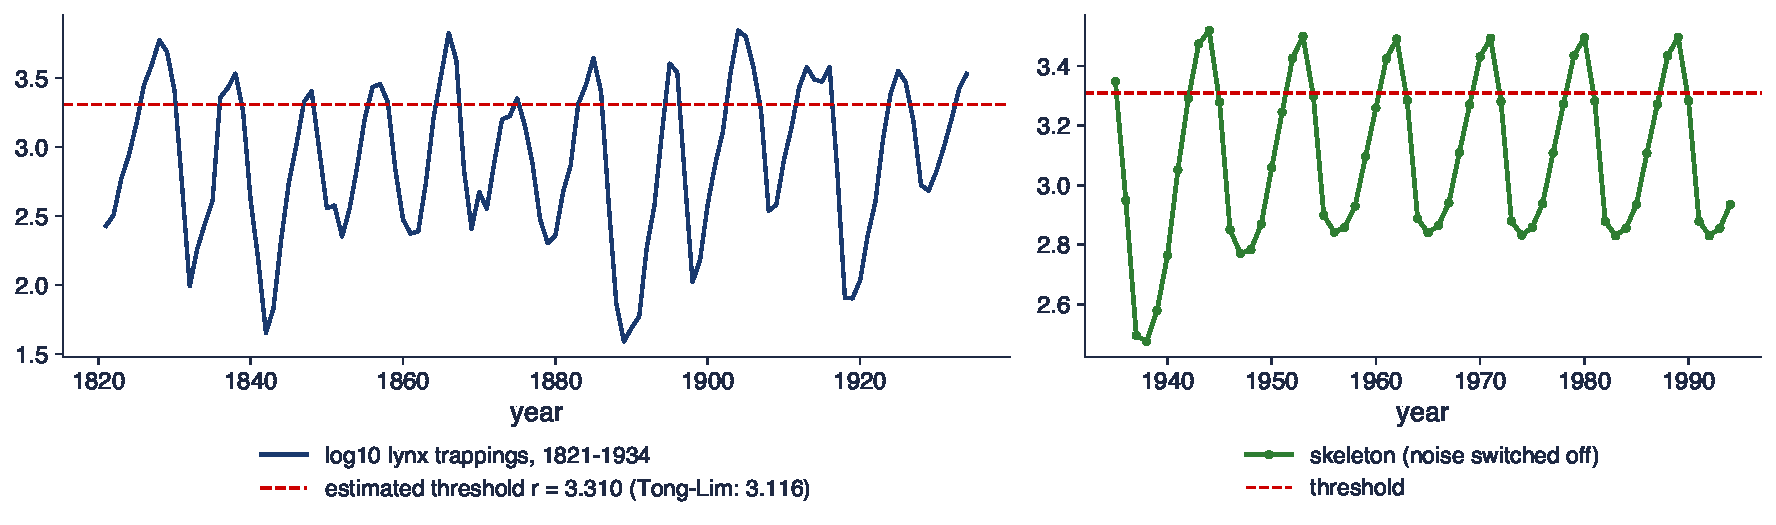
\includegraphics[width=0.97\textwidth,height=0.5\textheight,keepaspectratio]{ats_ch2_lynx.pdf}
\end{center}
\vspace{-0.25cm}
\begin{itemize}
    \item Left: data and the estimated threshold; right: the skeleton iterated 60 years from the last observations, noise switched off
\end{itemize}
\quantlet{ATS\_ch2\_lynx}{\qlurl{ATS_ch2_lynx}}
\end{frame}

\begin{frame}{Interpreting the lynx SETAR}
\itemsize{\small}
\begin{itemize}
    \item The skeleton settles on a stable limit cycle of period 9 years: the model produces the cycle without any noise
    \begin{itemize}
        \item a linear AR(11) needs noise to sustain the oscillation; its skeleton converges to the mean
    \end{itemize}
    \item The rise is slow (lower regime, seven lags), the fall is fast (upper regime, an explosive AR(2) on its own): the asymmetry of the data
    \item Residual variance 0.0352 against 0.0364 for AR(11): a small in-sample gain, a large gain in the description of the dynamics
\end{itemize}
\end{frame}

\begin{frame}{Case study: Hansen (1997), US unemployment}
\itemsize{\small}
\begin{itemize}
    \item The paper, Section 5: unemployment rate of men aged 20 and over (unemployed / labour force), monthly 1959.1--1996.7; $\Delta y_t$ on a constant and 12 lags \refHb
    \begin{itemize}
        \item $y_t$: the unemployment rate in \%; threshold variable $q_{t-1} = y_{t-1} - y_{t-d}$, $d = 2, \dots, 12$: the change over the last $d - 1$ months; trimming 15\%
        \item robust sup-Wald test, bootstrap $p$-values (1000 replications); the LS estimate $\hat d = 12$, $\hat\gamma = 0.302$, 95\% interval [0.213; 0.340], 314 and 124 observations
    \end{itemize}
    \item Our replication: the same construction from the BLS series on FRED (today's seasonal adjustment), the same model, $d = 12$
    \item Question: is there a ``recession regime'' with different dynamics, and how precisely is its threshold estimated?
\end{itemize}
\end{frame}

\begin{frame}{A threshold model for US unemployment}
\itemsize{\footnotesize}
\begin{center}
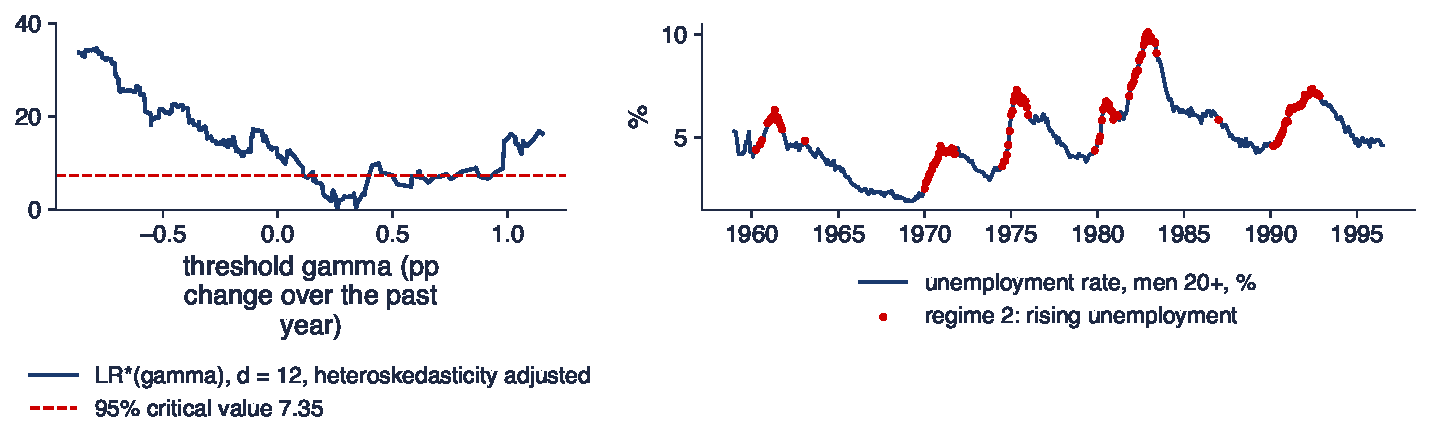
\includegraphics[width=0.97\textwidth,height=0.5\textheight,keepaspectratio]{ats_ch2_unemp_tar.pdf}
\end{center}
\vspace{-0.25cm}
\begin{itemize}
    \item Left: heteroskedasticity-adjusted $\mathrm{LR}^*(\gamma)$, $d = 12$; the 95\% set is where the curve lies below 7.35. Right: months in the rising-unemployment regime ($q_{t-1} > \hat\gamma$)
\end{itemize}
\quantlet{ATS\_ch2\_unemp\_tar}{\qlurl{ATS_ch2_unemp_tar}}
\end{frame}

\begin{frame}{Interpreting the unemployment TAR}
\itemsize{\footnotesize}
\begin{itemize}
    \item $\hat\gamma = 0.261$ pp (paper: 0.302), regimes of 314 and 124 months, the same split as in \refHb; 95\% set [0.131, 0.917]
    \begin{itemize}
        \item sup-Wald 47.2, bootstrap $p$ 0.015; linearity is rejected at 5\% for 10 of the 11 delays
    \end{itemize}
    \item Rising regime: intercept 0.065, AR(1) 0.18, AR(2) 0.28; other months: \ensuremath{-}0.019, \ensuremath{-}0.15, 0.06
    \begin{itemize}
        \item increases feed on themselves; in expansions unemployment is close to a random walk with a slight downward drift
    \end{itemize}
    \item With today's data the SSR is smallest at $d = 3$ ($\hat\gamma = \ensuremath{-}0.24$): the delay is fragile, the threshold effect is not; 1959--2019: $\hat\gamma = 0.261$, $p$ $<$\,0.001
\end{itemize}
\end{frame}

\begin{frame}{Recap: Threshold autoregression}
\itemsize{\small}
\begin{itemize}
    \item A piecewise-linear AR switching on an observed variable; can generate limit cycles
    \item $\hat\gamma$ super-consistent; slopes as if $\gamma$ were known
    \item Linearity tests need the bootstrap; threshold intervals invert LR with the value 7.35
    \item Lynx and unemployment: both landmark results replicate
\end{itemize}
\end{frame}


%=============================================================================
\section{Smooth transition autoregression}
%=============================================================================

\begin{frame}{STAR models (1/2)}
\itemsize{\small}
\begin{itemize}
    \item A weighted average of two AR regimes, with a weight $G$ that moves smoothly between 0 and 1 \refTer
    \begin{itemize}
        \item $y_t = \phi_1'\mathbf x_t[1 - G(s_t; \gamma, c)] + \phi_2'\mathbf x_t G(s_t; \gamma, c) + \varepsilon_t$, $\quad \mathbf x_t = (1, y_{t-1}, \dots, y_{t-p})'$
        \item $s_t$: the transition variable (e.g.\ a lag of $y_t$); $c$: the location of the transition; $\gamma > 0$: its speed
        \item $G = 0$: regime 1 with coefficients $\phi_1$; $G = 1$: regime 2 with $\phi_2$; in between, a mixture
    \end{itemize}
    \item A continuum of regimes
    \begin{itemize}
        \item smooth aggregation of many agents with different thresholds, or time aggregation, produces smooth switching
    \end{itemize}
\end{itemize}
\end{frame}

\begin{frame}{STAR models (2/2)}
\itemsize{\small}
\begin{itemize}
    \item \textbf{LSTAR} (logistic): low against high values of $s_t$
    \begin{itemize}
        \item $G = [1 + \exp\{-\gamma(s_t - c)/\hat\sigma_s\}]^{-1}$
        \item $\gamma \to \infty$ gives the TAR, $\gamma \to 0$ the linear AR; $\hat\sigma_s$: the standard deviation of $s_t$, which makes $\gamma$ scale free and easier to estimate
    \end{itemize}
    \item \textbf{ESTAR} (exponential): small against large \emph{deviations} from $c$, symmetric
    \begin{itemize}
        \item $G = 1 - \exp\{-\gamma(s_t - c)^2\}$
    \end{itemize}
    \item Survey with the modelling cycle (specification, estimation, evaluation): \refVDTF
\end{itemize}
\end{frame}

\begin{frame}{Testing linearity against STAR}
\itemsize{\small}
\begin{itemize}
    \item Under $H_0$: $\gamma = 0$, the parameters $c$ and $\phi_2$ are not identified: replace $G$ by a third-order Taylor expansion around $\gamma = 0$ \refLST
    \begin{itemize}
        \item auxiliary regression $\hat\varepsilon_t = \beta_0'\mathbf x_t + \beta_1'\tilde{\mathbf x}_t s_t + \beta_2'\tilde{\mathbf x}_t s_t^2 + \beta_3'\tilde{\mathbf x}_t s_t^3 + v_t$
        \item $\hat\varepsilon_t$: the residuals of the linear AR; $\tilde{\mathbf x}_t$: $\mathbf x_t$ without the constant; $\beta_k$: the coefficients of the interactions with $s_t^k$; $v_t$: the error
        \item LM3: $\beta_1 = \beta_2 = \beta_3 = 0$, an $F$ test with $3p$ restrictions; repeat for each candidate $s_t$ and take the smallest $p$-value (derivation in the \atsapplink{atsapp3}{atssrc3}{Appendix})
    \end{itemize}
    \item \textbf{Choice of the family} \refTer: test $H_{04}$: $\beta_3 = 0$, then $H_{03}$: $\beta_2 = 0 \mid \beta_3 = 0$, then $H_{02}$: $\beta_1 = 0 \mid \beta_2 = \beta_3 = 0$
    \begin{itemize}
        \item strongest rejection of $H_{03}$: ESTAR; of $H_{04}$ or $H_{02}$: LSTAR (an ESTAR has no cubic term in its expansion)
    \end{itemize}
    \item Estimation by nonlinear least squares, linear parameters concentrated out; evaluation by LM tests of no remaining nonlinearity and parameter constancy \refET
\end{itemize}
\end{frame}

\begin{frame}{Case study: van Dijk, Teräsvirta and Franses (2002)}
\itemsize{\small}
\begin{itemize}
    \item The paper, Section 7: unadjusted unemployment rate of US men aged 20+, June 1968--December 1999; estimation to 1989, forecasts for 1990--1999 \refVDTF
    \begin{itemize}
        \item $\Delta y_t$ on a constant, 11 monthly dummies, $y_{t-1}$ and 15 lags of $\Delta y_t$; transition variable $s_t = \Delta_{12}y_{t-d}$ (the 12-month change, lagged $d$ months), $d = 1, \dots, 6$
        \item their LSTAR with $d = 1$: $\hat\gamma = 23.15$, $\hat c = 0.27$, residual s.d.\ 0.92 of the AR
    \end{itemize}
    \item Our replication: the same series (BLS via FRED), sample, regressors and transition; the unrestricted lags, without their pruning of insignificant terms
    \item Question: does an LSTAR beat the linear model out of sample?
\end{itemize}
\end{frame}

\begin{frame}{An LSTAR for US unemployment}
\itemsize{\footnotesize}
\begin{center}
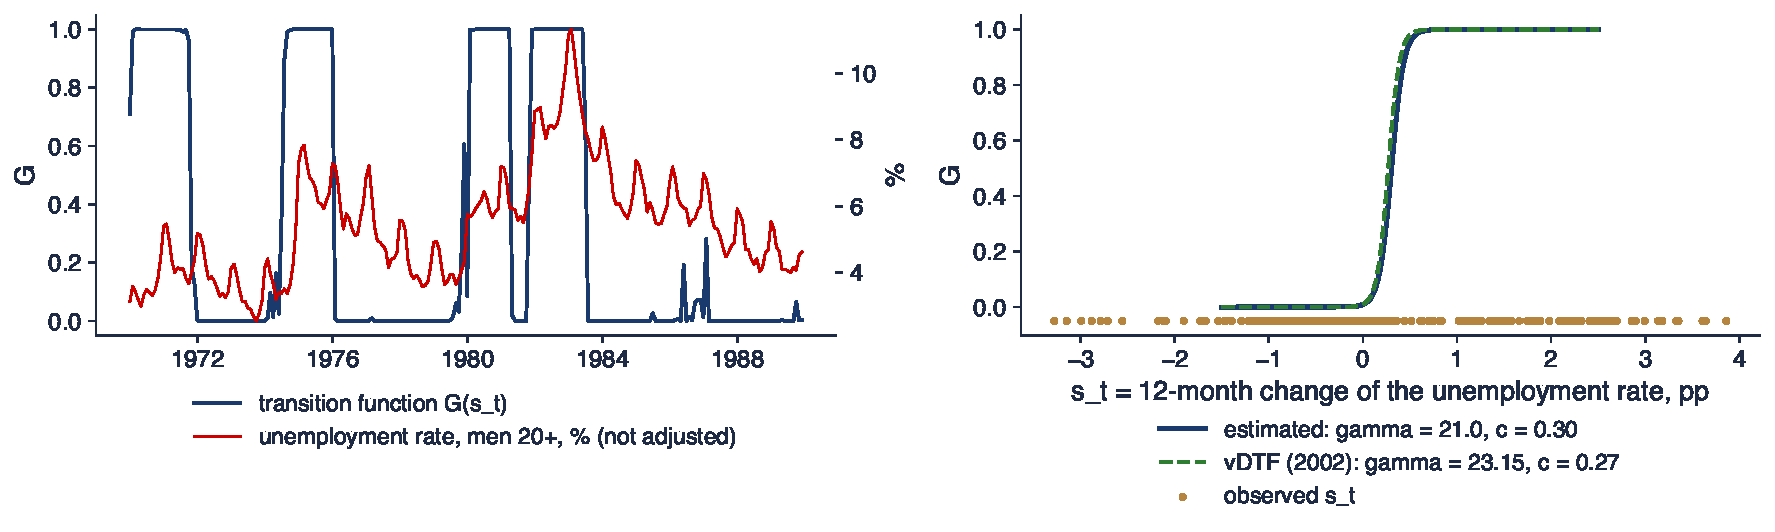
\includegraphics[width=0.97\textwidth,height=0.5\textheight,keepaspectratio]{ats_ch2_unemp_lstar.pdf}
\end{center}
\vspace{-0.25cm}
\begin{itemize}
    \item Left: the estimated transition function over time with the unemployment rate; right: $G$ as a function of $s_t = \Delta_{12}y_{t-1}$, ours and the published one
\end{itemize}
\quantlet{ATS\_ch2\_unemp\_lstar}{\qlurl{ATS_ch2_unemp_lstar}}
\end{frame}

\begin{frame}{Interpreting the LSTAR}
\itemsize{\footnotesize}
\begin{itemize}
    \item LM3 $p$-values: $d = 1$: 0.124, $d = 2$: 0.052, $d = 3$: 0.275; for $d = 2$: $H_{04}$ 0.008, $H_{03}$ 0.548, $H_{02}$ 0.461: LSTAR
    \begin{itemize}
        \item in line with \refVDTF: weak evidence, strongest for $d = 2$, pointing to the logistic family
    \end{itemize}
    \item $\hat\gamma = 21.0$, $\hat c = 0.30$, residual s.d.\ ratio 0.90; the regime switches when unemployment has risen by about 0.3 pp in a year ($G > 0.5$ in 32\% of months)
    \begin{itemize}
        \item AIC prefers the LSTAR (\ensuremath{-}3.034 against \ensuremath{-}2.979); BIC the linear model (\ensuremath{-}2.573 against \ensuremath{-}2.366): 18 extra parameters without pruning
    \end{itemize}
    \item 1990--1999, one step: RMSE 0.218 (LSTAR) against 0.228 (AR), HLN 1.14, $p$ 0.255: better, not significantly
\end{itemize}
\end{frame}

\begin{frame}{Real exchange rates and purchasing power parity}
\itemsize{\footnotesize}
\begin{columns}[T]
\begin{column}{0.34\textwidth}
\centering
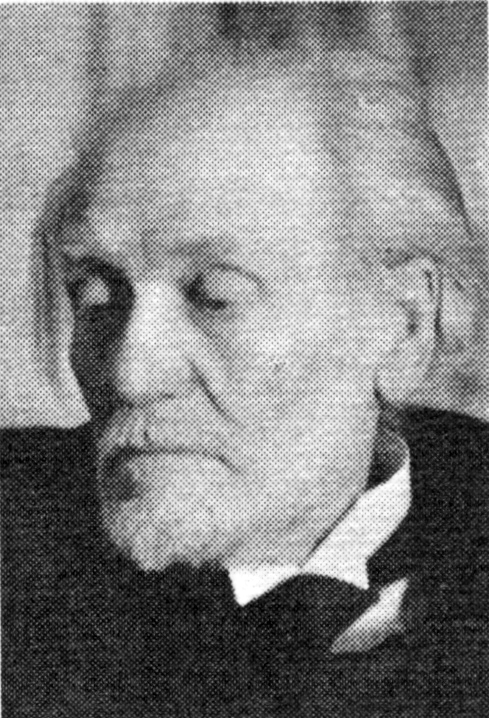
\includegraphics[height=0.24\textheight]{ch2_cassel.jpg}\\[1mm]
\imgcap{Gustav Cassel (1866--1945)}
\imgcredit{https://commons.wikimedia.org/wiki/File:Gustav_Cassel.jpg}{Portrait: unknown author; public domain; Wikimedia Commons}\\[1mm]\centering
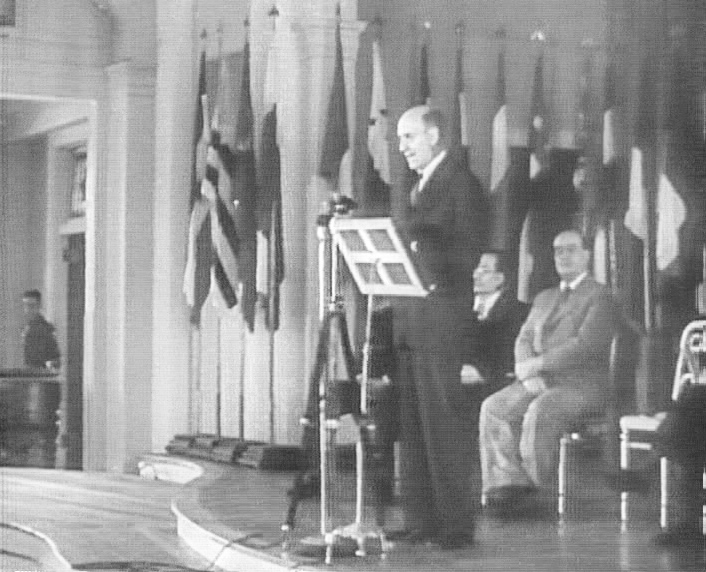
\includegraphics[height=0.15\textheight]{ch2_bretton_woods_1944.jpg}\\[1mm]
\imgcap{Bretton Woods, July 1944}
\imgcredit{https://commons.wikimedia.org/wiki/File:Morgenthau_Bretton_Woods_opening_1944.jpg}{Photo: US National Archives (1944); public domain; Wikimedia Commons}
\end{column}
\begin{column}{0.64\textwidth}
\begin{itemize}
    \item Purchasing power parity, PPP (\refCas): the real exchange rate $q_t = s_t - p_t + p_t^*$ should be stationary
    \begin{itemize}
        \item $s_t$: the log nominal rate (domestic per foreign currency); $p_t$, $p_t^*$: log domestic and foreign price levels
        \item after Bretton Woods ended (1973) unit-root tests rarely reject
        \item first PPP puzzle: no mean reversion; second: half-lives of 3--5 years, too slow for nominal shocks
    \end{itemize}
    \item Transaction costs create a band of inaction: near parity $q_t$ is close to a random walk, far from it arbitrage pulls it back \refMNP
    \begin{itemize}
        \item \refTPS: ESTAR $q_t - \mu = (q_{t-1} - \mu)\exp\{-\theta^2(q_{t-1} - \mu)^2\} + \varepsilon_t$
        \item $\mu$: the equilibrium; near it the AR coefficient $\exp\{\cdot\}$ is close to 1 (random walk), far from it close to 0 (fast reversion); $\theta^2$: the speed
    \end{itemize}
\end{itemize}
\end{column}
\end{columns}
\end{frame}

\begin{frame}{Case study: Taylor, Peel and Sarno (2001)}
\itemsize{\small}
\begin{itemize}
    \item The paper: monthly real dollar rates of sterling, mark, franc and yen, 1973M01--1996M12, IMF IFS data, $q(1973M01) = 0$; ESTAR with $p = d = 1$ and $\beta_1 = -\beta_1^* = 1$ (eq.\ 8) \refTPS
    \begin{itemize}
        \item dollar--sterling: $\hat\theta^2 = 0.452$, $\hat\mu = -0.149$, $s = 0.033$ (residual standard deviation); Monte Carlo $p$-value of $\hat\theta$ under a random walk: 0.002
        \item half-lives from generalised impulse responses conditional on the average history: under one year for a 40\% shock, just under three years for 1\%
    \end{itemize}
    \item Our replication for dollar--sterling: end-of-month DEXUSUK, US CPI (CPIAUCNS), UK CPI (OECD to 1987, then ONS); same model, same half-life procedure; extension to August 2026
    \item Question: is the real exchange rate nonlinearly mean reverting, and how fast?
\end{itemize}
\end{frame}

\begin{frame}{Nonlinear mean reversion of the real dollar--sterling rate}
\itemsize{\footnotesize}
\begin{center}
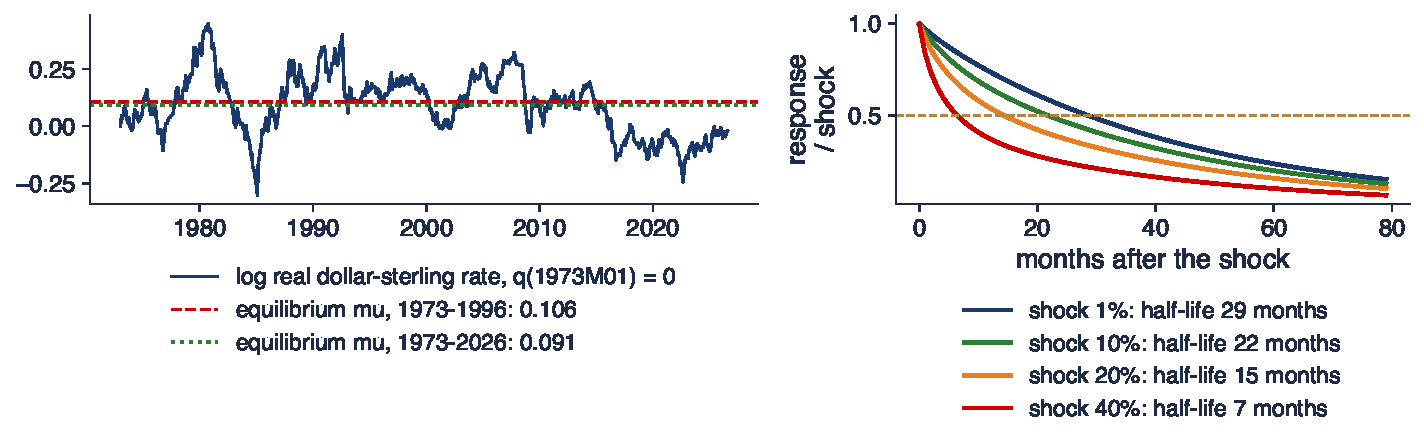
\includegraphics[width=0.97\textwidth,height=0.5\textheight,keepaspectratio]{ats_ch2_ppp_estar.pdf}
\end{center}
\vspace{-0.25cm}
\begin{itemize}
    \item Left: $q_t$ and the estimated equilibria; right: generalised impulse responses of the 1973--1996 ESTAR, shocks of 1--40\%, averaged over the observed histories
\end{itemize}
\quantlet{ATS\_ch2\_ppp\_estar}{\qlurl{ATS_ch2_ppp_estar}}
\end{frame}

\begin{frame}{Interpreting the ESTAR}
\itemsize{\footnotesize}
\begin{itemize}
    \item 1973--1996: $\hat\theta^2 = 0.527$ (s.e.\ 0.219), $\hat\mu = 0.106$, $s = 0.033$; Monte Carlo $p$-value of the $t$-ratio 0.165 (paper: 0.002)
    \begin{itemize}
        \item $\theta^2$ and $s$ are close to the paper; $\mu$ differs because the UK CPI of the paper (IFS) is not the series published today
    \end{itemize}
    \item Half-lives: 1\% shock 29 months, 10\% 22, 40\% 7; linear AR(1): 21 months; from equilibrium: 42 months for 1\%
    \begin{itemize}
        \item large deviations die out fast: the second PPP puzzle is a feature of small shocks
    \end{itemize}
    \item Dickey--Fuller: \ensuremath{-}2.20 ($p$ 0.205); its power against our ESTAR is 19\%
    \item KSS \refKSS: \ensuremath{-}2.47 ($p$ 0.144) to 1996, \ensuremath{-}3.47 ($p$ 0.014) to 2026
    \begin{itemize}
        \item the $t$ statistic of $\delta$ in $\Delta q_t = \delta q_{t-1}^3 + e_t$ (demeaned $q_t$): a unit-root test against a stationary ESTAR; reject in the left tail
    \end{itemize}
\end{itemize}
\end{frame}

\begin{frame}{Recap: Smooth transition}
\itemsize{\small}
\begin{itemize}
    \item LSTAR: asymmetry between low and high states; ESTAR: small and large deviations
    \item LM tests from a Taylor expansion avoid the identification problem; the sequence $H_{04}$, $H_{03}$, $H_{02}$ chooses the family
    \item Unemployment: the published LSTAR replicates; its forecast gain is small
    \item PPP: half-lives depend on the size of the shock; the evidence for nonlinearity depends on the sample
\end{itemize}
\end{frame}


%=============================================================================
\section{Nonlinearity tests}
%=============================================================================

\begin{frame}{General and specific tests}
\itemsize{\small}
\begin{itemize}
    \item \textbf{BDS} \refBDSL: correlation integral $C_{m}(\varepsilon)$ of $m$-histories; under i.i.d.\ $C_m = C_1^m$; applied to the residuals of a linear model
    \begin{itemize}
        \item $C_m(\varepsilon)$: the share of pairs of $m$-histories $(y_t, \dots, y_{t+m-1})$ that are within distance $\varepsilon$ in every coordinate
        \item power against any dependence left in the residuals, including ARCH: a rejection does not say which nonlinearity
    \end{itemize}
    \item \textbf{Keenan} (squared fitted values) and the test of \refTsa\ (all cross products $y_{t-i}y_{t-j}$, orthogonalised): $F$ tests of second-order Volterra terms
    \begin{itemize}
        \item Tsay's arranged-autoregression test targets the TAR alternative \refTsb
    \end{itemize}
    \item \textbf{LM3} (STAR) and \textbf{sup-Wald} (TAR): specific alternatives, more power when they are right
    \begin{itemize}
        \item caution: structural breaks, outliers and heteroskedasticity also reject linearity \refCar
    \end{itemize}
\end{itemize}
\end{frame}

\begin{frame}{Five series, five tests}
\itemsize{\footnotesize}
\begin{center}
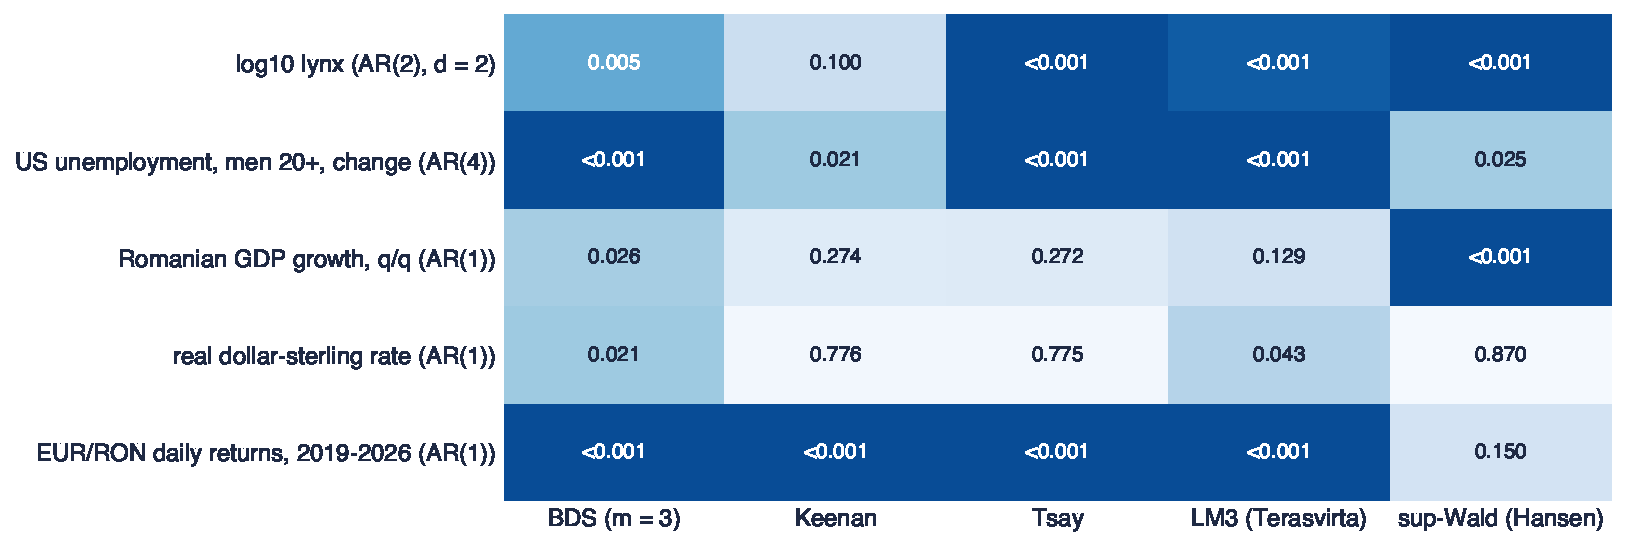
\includegraphics[width=0.97\textwidth,height=0.5\textheight,keepaspectratio]{ats_ch2_nonlinearity_tests.pdf}
\end{center}
\vspace{-0.25cm}
\begin{itemize}
    \item $p$-values; darker: stronger rejection of linearity. BDS on the AR residuals ($m = 3$, $\varepsilon = \hat\sigma$); LM3 and sup-Wald with $s = q = y_{t-d}$; sup-Wald with 200 bootstrap replications
\end{itemize}
\quantlet{ATS\_ch2\_nonlinearity\_tests}{\qlurl{ATS_ch2_nonlinearity_tests}}
\end{frame}

\begin{frame}{Interpreting the test battery}
\itemsize{\small}
\begin{itemize}
    \item Lynx and unemployment: every specific test rejects; the nonlinearity is real and of the threshold type
    \item EUR/RON returns: BDS, Keenan, Tsay and LM3 all reject with $p$ $<$\,0.001, yet the TAR sup-Wald does not ($p$ 0.150)
    \begin{itemize}
        \item volatility clustering and outliers, not a nonlinear conditional mean: the heteroskedasticity-robust test is the honest one
    \end{itemize}
    \item Romanian GDP growth: only BDS and sup-Wald reject ($p$ $<$\,0.001): the 2009 and 2020 quarters act as a ``regime''; a break or an outlier model may explain the same data
\end{itemize}
\end{frame}

\begin{frame}{Threshold cointegration}
\itemsize{\small}
\begin{itemize}
    \item \refBF: the error-correction term $z_t = y_t - \beta x_t$ adjusts only outside a band: $\Delta z_t = \rho\,z_{t-1}\mathbf 1\{|z_{t-1}| > \gamma\} + \varepsilon_t$
    \begin{itemize}
        \item $y_t, x_t$: two cointegrated prices; $\beta$: the cointegrating coefficient; $\rho < 0$: the speed of adjustment outside the band $[-\gamma, \gamma]$
        \item the same transaction-cost argument as ESTAR, for a pair of prices: commodity prices in two markets, interest-rate pass-through, the law of one price
    \end{itemize}
    \item Asymmetric adjustment (momentum TAR) \refES; the test of linear against threshold VECM with a bootstrap \refHS
    \begin{itemize}
        \item \atschlink{https://danpele.github.io/Advanced-Time-Series/EN/Courses/chapter4_cointegration_vecm_ardl_panel.pdf}{Chapter 4} introduces the linear VECM and ARDL; threshold versions are a natural project extension
    \end{itemize}
    \item Romanian example: pass-through from the BNR policy rate to ROBOR and to lending rates, with a band where banks do not adjust
\end{itemize}
\end{frame}


%=============================================================================
\section{Forecasting with nonlinear models}
%=============================================================================

\begin{frame}{Multi-step forecasts are not the skeleton}
\itemsize{\small}
\begin{itemize}
    \item For $h = 1$: $\E(y_{t+1}\mid\mathcal F_t) = F(\mathbf y_t)$; for $h \ge 2$: $\E[F(F(\mathbf y_t) + \varepsilon_{t+1}, \dots)] \ne F(F(\mathbf y_t))$ (Jensen)
    \begin{itemize}
        \item $F$: the conditional mean function of the model; Jensen: the mean of a nonlinear function is not the function of the mean
        \item iterating the skeleton (the ``naive'' forecast) is biased; simulate paths with bootstrapped residuals and average them \refCFS
        \item the predictive density can be skewed or bimodal: report densities, scored by the CRPS or the log score (\atschlink{https://danpele.github.io/Advanced-Time-Series/EN/Courses/chapter1_forecast_evaluation.pdf}{Chapter 1})
    \end{itemize}
    \item Evidence: nonlinear models rarely beat linear ones on average; gains concentrate in particular regimes (recessions) \refMZTT, \refTDM
    \begin{itemize}
        \item evaluate conditionally: GW tests with the regime as instrument (\atschlink{https://danpele.github.io/Advanced-Time-Series/EN/Courses/chapter1_forecast_evaluation.pdf}{Chapter 1}); asymmetric dynamics in US unemployment \refKPo
    \end{itemize}
\end{itemize}
\end{frame}

\begin{frame}{TAR and AR forecasts of US unemployment}
\itemsize{\footnotesize}
\begin{center}
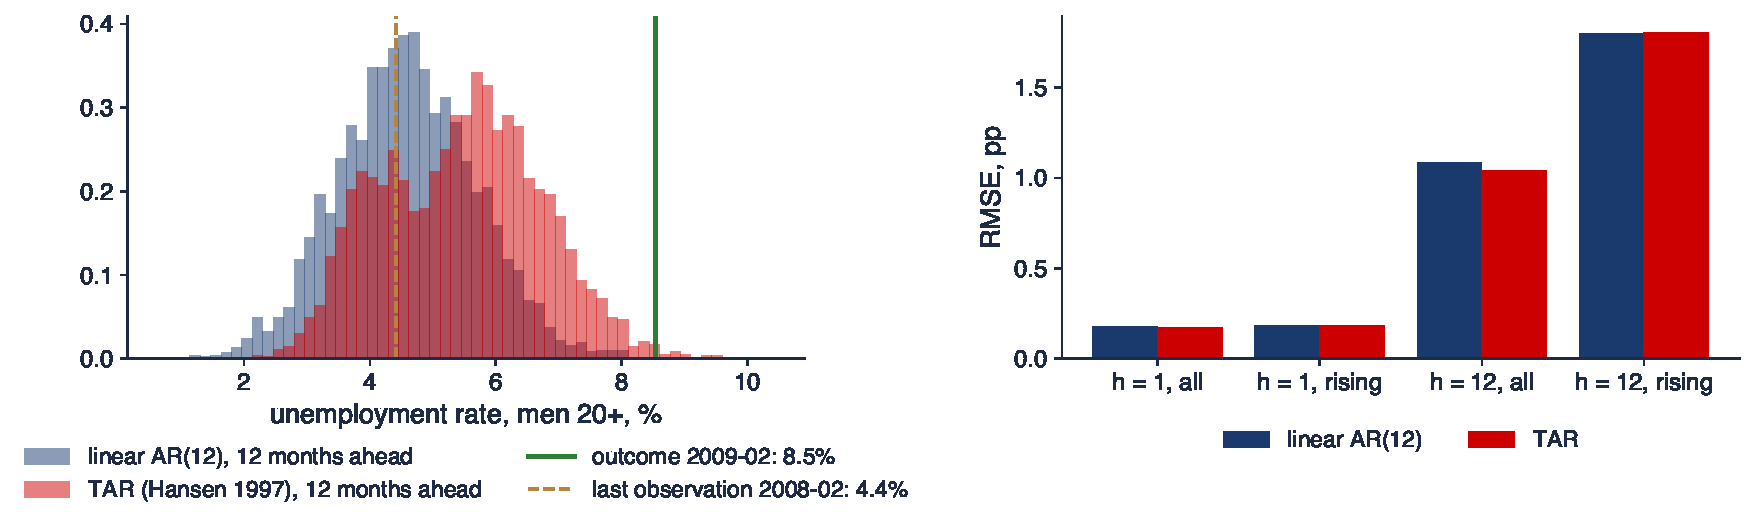
\includegraphics[width=0.97\textwidth,height=0.5\textheight,keepaspectratio]{ats_ch2_nonlinear_forecasts.pdf}
\end{center}
\vspace{-0.25cm}
\begin{itemize}
    \item Hansen's TAR ($d = 12$) and a linear AR(12) in differences, parameters fixed at 1959--1996; forecasts of the level by 500 simulated paths, origins 1996--2019. Left: 12-month densities from February 2008
\end{itemize}
\quantlet{ATS\_ch2\_nonlinear\_forecasts}{\qlurl{ATS_ch2_nonlinear_forecasts}}
\end{frame}

\begin{frame}{Interpreting the nonlinear forecasts}
\itemsize{\small}
\begin{itemize}
    \item From February 2008 (before the 2008--2009 surge): TAR mean 5.5\%, 90\% range [3.5; 7.5]; AR mean 4.6\%, [2.9; 6.4]; outcome 8.5\%
    \begin{itemize}
        \item the TAR density is skewed upwards once unemployment starts rising; neither model foresaw the size of the recession
    \end{itemize}
    \item $P = 270$ months: RMSE at 1 month 0.173 (TAR) against 0.177 (AR), HLN 1.12 ($p$ 0.265); at 12 months 1.039 against 1.087 ($p$ 0.599)
    \begin{itemize}
        \item in the 62 rising-regime months the two are equal at 12 months (1.802 and 1.801): no regime-specific gain out of sample
    \end{itemize}
    \item A good in-sample nonlinearity is not a forecasting gain: pre-register the comparison
\end{itemize}
\end{frame}

\begin{frame}{Recap: Nonlinearity tests and forecasts}
\itemsize{\small}
\begin{itemize}
    \item General tests (BDS, Keenan, Tsay) detect, specific ones (LM3, sup-Wald) describe
    \item Heteroskedasticity, outliers and breaks also reject linearity
    \item Multi-step nonlinear forecasts need simulation; report densities
    \item Out of sample, nonlinear models gain little on average; test where they should gain
\end{itemize}
\end{frame}


%=============================================================================
\section{AI for scientific discovery}
%=============================================================================

\begin{frame}{An open question}
\itemsize{\small}
\begin{itemize}
    \item Nonlinearity or breaks? A few shifts of the mean can look like nonlinear mean reversion, and a threshold model can look like a sequence of breaks \refCar, \refDI
    \begin{itemize}
        \item formal: is the KSS (ESTAR) rejection for the real dollar--sterling rate robust to Bai--Perron mean regimes estimated on the same data?
        \item falsified if the rejection disappears once the null distribution accounts for the estimated breaks
    \end{itemize}
    \item Why it matters: half-lives, PPP and the credibility of exchange-rate models depend on which story is true
    \begin{itemize}
        \item literature to start from: \refTPS, \refKSS, \refMNP, \refCar, \refBPb
    \end{itemize}
\end{itemize}
\end{frame}

\begin{frame}{The discovery loop with an AI assistant}
\itemsize{\footnotesize}
\begin{itemize}
    \item An AI assistant (an LLM such as Claude, ChatGPT, Gemini or Copilot) speeds up each step; Semantic Scholar and Elicit help with the literature
    \begin{itemize}
        \item \textbf{literature}: \aiprompt{List peer-reviewed papers that test ESTAR real exchange rate models allowing for breaks in the mean; give DOIs.} Then check every DOI on Crossref
        \item \textbf{hypothesis}: \aiprompt{Propose a data-generating process with mean breaks and no nonlinearity that makes the KSS test reject.}
        \item \textbf{code and replication}: reproduce first a number of this lecture (the KSS statistic to 2026), then the new procedure
        \item \textbf{robustness and critique}: \aiprompt{Act as a referee: list every way in which estimating breaks on the same data biases the test.}
    \end{itemize}
    \item Report: what was asked, what was kept, what was rejected (AI\_USE.md, AI\_ERRORS.md)
\end{itemize}
\end{frame}

\begin{frame}{Required checks}
\itemsize{\small}
\begin{itemize}
    \item Every reference exists and says what is claimed (DOI resolves, title matches, the result is in the paper)
    \item The null distribution reproduces the whole procedure: breaks estimated on each simulated series, not fixed at the observed dates
    \item The number of breaks, the trimming and the criterion (BIC) are fixed before seeing the test result
    \item The data are the published series (vintage, deflator, end of month); differences from the paper are reported
    \item ``Not significant within regimes'' is not ``linear'': report the power of the procedure
\end{itemize}
\end{frame}

\begin{frame}{Mini-case: ESTAR evidence or mean shifts?}
\itemsize{\footnotesize}
\begin{center}
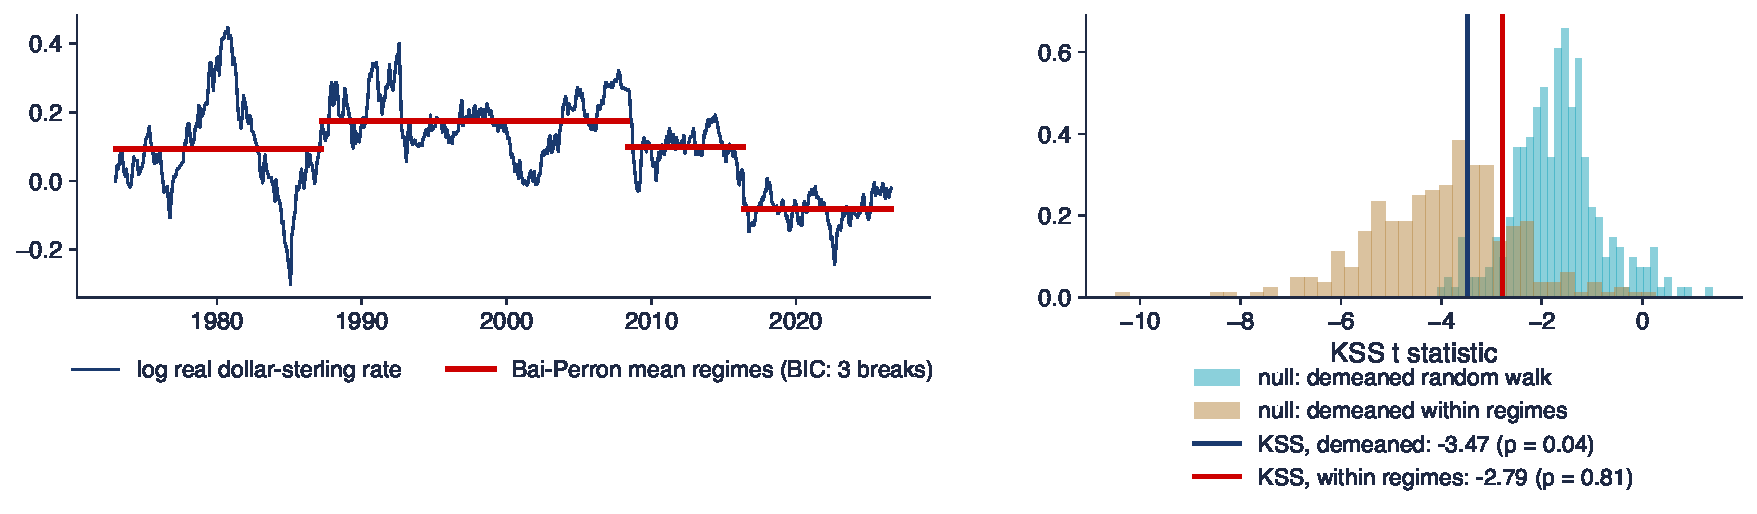
\includegraphics[width=0.97\textwidth,height=0.46\textheight,keepaspectratio]{ats_ch2_ai_case.pdf}
\end{center}
\vspace{-0.25cm}
\begin{itemize}
    \item Left: real dollar--sterling rate with Bai--Perron mean regimes (BIC: three breaks, March 1987, May 2008, May 2016); right: KSS null distributions from 300 random walks put through the same steps
    \item Demeaned: KSS \ensuremath{-}3.47, $p$ 0.037 (5\%: \ensuremath{-}3.13); within regimes: \ensuremath{-}2.79, $p$ 0.813 (5\%: \ensuremath{-}6.30): the evidence for ESTAR disappears once the break search is part of the null
\end{itemize}
\quantlet{ATS\_ch2\_ai\_case}{\qlurl{ATS_ch2_ai_case}}
\end{frame}

\begin{frame}{Project idea}
\itemsize{\small}
\begin{itemize}
    \item \textbf{Regimes in Romanian inflation and the policy rate}: breaks, thresholds or both?
    \begin{itemize}
        \item replicate first: the Bai--Perron dates of this lecture and the TAR test of \refHb\ on the US data
        \item extension: an AR model of Romanian inflation with a partial break in the intercept against an LSTAR in the 12-month change of inflation; pre-register the comparison (1--12 months, CRPS, \refHolm)
        \item optional: threshold pass-through from the BNR rate to ROBOR (\atschlink{https://danpele.github.io/Advanced-Time-Series/EN/Courses/chapter4_cointegration_vecm_ardl_panel.pdf}{Chapter 4})
    \end{itemize}
    \item Deliverables follow the course rules: repository, report, AI\_USE.md, AI\_ERRORS.md, oral defence
\end{itemize}
\end{frame}


%=============================================================================
\section{Wrap-up}
%=============================================================================

\begin{frame}{Key takeaways}
\itemsize{\small}
\begin{itemize}
    \item A break date chosen from the data is a nuisance parameter: use sup/exp/ave tests with their own critical values
    \item Bai--Perron: global LS by dynamic programming, UDmax and sequential tests, BIC/LWZ, intervals for the dates
    \item Monitor with a CSW boundary; test variance breaks with $\kappa_2$; bootstrap unit-root tests with breaks
    \item TAR and STAR: test with the bootstrap or LM expansions, estimate by concentrated (N)LS, forecast by simulation
    \item Breaks and nonlinearity mimic each other: test one allowing for the other
\end{itemize}
\end{frame}

\begin{frame}{Self-assessment}
\itemsize{\small}
\begin{columns}[T]
\begin{column}{0.56\textwidth}
\begin{block}{Questions}
\begin{itemize}
    \item Why is the 5\% critical value of sup-Wald with one coefficient above 8, not 3.84?
    \item What does dynamic programming save in the Bai--Perron estimator?
    \item Why does a repeated 5\% test eventually raise a false alarm?
    \item Why is the threshold of a TAR estimated at rate $T$?
    \item When does the half-life of an ESTAR depend on the shock?
\end{itemize}
\end{block}
\end{column}
\begin{column}{0.40\textwidth}
\begin{block}{Next: SVAR and local projections}
\begin{itemize}
    \item Structural VAR and local projections: identification of shocks
    \item State-dependent local projections extend this chapter's nonlinear models to impulse responses
\end{itemize}
\end{block}
\end{column}
\end{columns}
\end{frame}


%=============================================================================
\section{Appendix}
%=============================================================================

\begin{frame}{Appendix: the limit of the sup-Wald statistic}
\hypertarget{atsapp1}{}\atsappback{atssrc1}{Back}
\itemsize{\small}
\begin{itemize}
    \item Mean shift, $\sigma^2$ known: $W_T(\pi) = \dfrac{T\pi(1 - \pi)(\bar y_1 - \bar y_2)^2}{\sigma^2}$, $\bar y_1$, $\bar y_2$ the means before and after $[\pi T]$
    \item With $S_T(r) = \sigma^{-1}T^{-1/2}\sum_{t \le [rT]}(y_t - \mu) \Rightarrow B(r)$ (FCLT, \atschlink{https://danpele.github.io/Advanced-Time-Series/EN/Courses/chapter0_refresher_inference.pdf}{Chapter 0}): $\bar y_1 - \bar y_2 = \dfrac{\sigma}{\sqrt T}\Big[\dfrac{S_T(\pi)}{\pi} - \dfrac{S_T(1) - S_T(\pi)}{1 - \pi}\Big]$
    \item The bracket equals $\dfrac{S_T(\pi) - \pi S_T(1)}{\pi(1 - \pi)}$, so $W_T(\pi) \Rightarrow \dfrac{[B(\pi) - \pi B(1)]^2}{\pi(1 - \pi)}$, a squared Brownian bridge over its variance
    \item The continuous mapping theorem gives the limit of $\sup_{\pi \in \Pi}$; with $p$ coefficients, $B$ is $p$-dimensional; with an unknown $\sigma^2$ or a HAC variance the limit is the same
\end{itemize}
\end{frame}

\begin{frame}{Appendix: the critical value 7.35 of the threshold LR}
\hypertarget{atsapp2}{}\atsappback{atssrc2}{Back}
\itemsize{\small}
\begin{itemize}
    \item \refHc: with a shrinking threshold effect, $\mathrm{LR}_T(\gamma_0) \to_d \eta^2\xi$, $\xi = \max_{s}[2W(s) - |s|]$, $W$ a two-sided Brownian motion
    \item For one side, $\max_{s \ge 0}[2W(s) - s]$ is exponential with mean 2: $P(\cdot \le x) = 1 - e^{-x/2}$ (the maximum of a Brownian motion with drift)
    \item The two sides are independent: $P(\xi \le x) = (1 - e^{-x/2})^2$; solving $(1 - e^{-x/2})^2 = 1 - \alpha$ gives $c(\alpha) = -2\ln(1 - \sqrt{1 - \alpha})$
    \item $c(0.10) = 5.94$, $c(0.05) = 7.35$, $c(0.01) = 10.59$; under heteroskedasticity divide LR by $\hat\eta^2$ before comparing
\end{itemize}
\end{frame}

\begin{frame}{Appendix: the Taylor expansion behind LM3}
\hypertarget{atsapp3}{}\atsappback{atssrc3}{Back}
\itemsize{\small}
\begin{itemize}
    \item LSTAR: $G(s; \gamma, c) - \tfrac12 = \tfrac14\gamma(s - c) - \tfrac{1}{48}\gamma^3(s - c)^3 + O(\gamma^5)$ around $\gamma = 0$ (with $\hat\sigma_s = 1$)
    \item Substituting in $\phi_1'\mathbf x_t + (\phi_2 - \phi_1)'\mathbf x_t G$ and collecting powers of $s_t$ gives $\beta_0'\mathbf x_t + \sum_{k=1}^3\beta_k'\tilde{\mathbf x}_t s_t^k$, every $\beta_k$ proportional to $\gamma$
    \item So $H_0$: $\gamma = 0$ becomes $\beta_1 = \beta_2 = \beta_3 = 0$, testable without estimating $c$; the first-order expansion (LM1) has no power when only the intercept switches \refLST
    \item ESTAR: $1 - e^{-\gamma(s - c)^2} = \gamma(s - c)^2 + O(\gamma^2)$: squares only, hence the decision rule of \refTer
\end{itemize}
\end{frame}


%=============================================================================
\section{References}
%=============================================================================

\begin{frame}{References (1/7)}
\itemsize{\tiny}
\begin{itemize}
    \item Andrews, D. W. K. (1993). Tests for parameter instability and structural change with unknown change point. \textit{Econometrica}, 61(4), 821--856. \href{https://doi.org/10.2307/2951764}{doi:10.2307/2951764}
    \item Andrews, D. W. K., \& Ploberger, W. (1994). Optimal tests when a nuisance parameter is present only under the alternative. \textit{Econometrica}, 62(6), 1383--1414. \href{https://doi.org/10.2307/2951753}{doi:10.2307/2951753}
    \item Bai, J. (1997). Estimation of a change point in multiple regression models. \textit{The Review of Economics and Statistics}, 79(4), 551--563. \href{https://doi.org/10.1162/003465397557132}{doi:10.1162/003465397557132}
    \item Bai, J., \& Perron, P. (1998). Estimating and testing linear models with multiple structural changes. \textit{Econometrica}, 66(1), 47--78. \href{https://doi.org/10.2307/2998540}{doi:10.2307/2998540}
    \item Bai, J., \& Perron, P. (2003). Computation and analysis of multiple structural change models. \textit{Journal of Applied Econometrics}, 18(1), 1--22. \href{https://doi.org/10.1002/jae.659}{doi:10.1002/jae.659}
    \item Balke, N. S., \& Fomby, T. B. (1997). Threshold cointegration. \textit{International Economic Review}, 38(3), 627--645. \href{https://doi.org/10.2307/2527284}{doi:10.2307/2527284}
    \item Brock, W. A., Dechert, W. D., Scheinkman, J. A., \& LeBaron, B. (1996). A test for independence based on the correlation dimension. \textit{Econometric Reviews}, 15(3), 197--235. \href{https://doi.org/10.1080/07474939608800353}{doi:10.1080/07474939608800353}
    \item Brown, R. L., Durbin, J., \& Evans, J. M. (1975). Techniques for testing the constancy of regression relationships over time. \textit{Journal of the Royal Statistical Society, Series B}, 37(2), 149--192. \href{https://doi.org/10.1111/j.2517-6161.1975.tb01532.x}{doi:10.1111/j.2517-6161.1975.tb01532.x}
    \item Carrasco, M. (2002). Misspecified structural change, threshold, and Markov-switching models. \textit{Journal of Econometrics}, 109(2), 239--273. \href{https://doi.org/10.1016/S0304-4076(02)00112-4}{doi:10.1016/S0304-4076(02)00112-4}
    \item Casini, A., \& Perron, P. (2019). Structural breaks in time series. In \textit{Oxford Research Encyclopedia of Economics and Finance}. Oxford University Press. \href{https://doi.org/10.1093/acrefore/9780190625979.013.179}{doi:10.1093/acrefore/9780190625979.013.179}
    \item Cassel, G. (1918). Abnormal deviations in international exchanges. \textit{The Economic Journal}, 28(112), 413--415. \href{https://doi.org/10.2307/2223329}{doi:10.2307/2223329}
\end{itemize}
\end{frame}

\begin{frame}{References (2/7)}
\itemsize{\tiny}
\begin{itemize}
    \item Chan, K. S. (1993). Consistency and limiting distribution of the least squares estimator of a threshold autoregressive model. \textit{The Annals of Statistics}, 21(1), 520--533. \href{https://doi.org/10.1214/aos/1176349040}{doi:10.1214/aos/1176349040}
    \item Chow, G. C. (1960). Tests of equality between sets of coefficients in two linear regressions. \textit{Econometrica}, 28(3), 591--605. \href{https://doi.org/10.2307/1910133}{doi:10.2307/1910133}
    \item Chu, C.-S. J., Hornik, K., \& Kuan, C.-M. (1995). MOSUM tests for parameter constancy. \textit{Biometrika}, 82(3), 603--617. \href{https://doi.org/10.1093/biomet/82.3.603}{doi:10.1093/biomet/82.3.603}
    \item Chu, C.-S. J., Stinchcombe, M., \& White, H. (1996). Monitoring structural change. \textit{Econometrica}, 64(5), 1045--1065. \href{https://doi.org/10.2307/2171955}{doi:10.2307/2171955}
    \item Clements, M. P., Franses, P. H., \& Swanson, N. R. (2004). Forecasting economic and financial time-series with non-linear models. \textit{International Journal of Forecasting}, 20(2), 169--183. \href{https://doi.org/10.1016/j.ijforecast.2003.10.004}{doi:10.1016/j.ijforecast.2003.10.004}
    \item Clements, M. P., \& Hendry, D. F. (1998). \textit{Forecasting Economic Time Series}. Cambridge University Press. \href{https://doi.org/10.1017/CBO9780511599286}{doi:10.1017/CBO9780511599286}
    \item Clements, M. P., \& Hendry, D. F. (2006). Forecasting with breaks. In G. Elliott, C. W. J. Granger, \& A. Timmermann (Eds.), \textit{Handbook of Economic Forecasting} (Vol.\ 1, pp.\ 605--657). Elsevier. \href{https://doi.org/10.1016/S1574-0706(05)01012-8}{doi:10.1016/S1574-0706(05)01012-8}
    \item Davies, R. B. (1987). Hypothesis testing when a nuisance parameter is present only under the alternative. \textit{Biometrika}, 74(1), 33--43. \href{https://doi.org/10.1093/biomet/74.1.33}{doi:10.1093/biomet/74.1.33}
    \item Diebold, F. X., \& Inoue, A. (2001). Long memory and regime switching. \textit{Journal of Econometrics}, 105(1), 131--159. \href{https://doi.org/10.1016/S0304-4076(01)00073-2}{doi:10.1016/S0304-4076(01)00073-2}
    \item Diebold, F. X., \& Mariano, R. S. (1995). Comparing predictive accuracy. \textit{Journal of Business \& Economic Statistics}, 13(3), 253--263. \href{https://doi.org/10.1080/07350015.1995.10524599}{doi:10.1080/07350015.1995.10524599}
    \item van Dijk, D., Teräsvirta, T., \& Franses, P. H. (2002). Smooth transition autoregressive models: A survey of recent developments. \textit{Econometric Reviews}, 21(1), 1--47. \href{https://doi.org/10.1081/ETC-120008723}{doi:10.1081/ETC-120008723}
\end{itemize}
\end{frame}

\begin{frame}{References (3/7)}
\itemsize{\tiny}
\begin{itemize}
    \item Eitrheim, Ø., \& Teräsvirta, T. (1996). Testing the adequacy of smooth transition autoregressive models. \textit{Journal of Econometrics}, 74(1), 59--75. \href{https://doi.org/10.1016/0304-4076(95)01751-8}{doi:10.1016/0304-4076(95)01751-8}
    \item Enders, W., \& Siklos, P. L. (2001). Cointegration and threshold adjustment. \textit{Journal of Business \& Economic Statistics}, 19(2), 166--176. \href{https://doi.org/10.1198/073500101316970395}{doi:10.1198/073500101316970395}
    \item Fryzlewicz, P. (2014). Wild binary segmentation for multiple change-point detection. \textit{The Annals of Statistics}, 42(6), 2243--2281. \href{https://doi.org/10.1214/14-AOS1245}{doi:10.1214/14-AOS1245}
    \item Garcia, R., \& Perron, P. (1996). An analysis of the real interest rate under regime shifts. \textit{The Review of Economics and Statistics}, 78(1), 111--125. \href{https://doi.org/10.2307/2109851}{doi:10.2307/2109851}
    \item Giacomini, R., \& Rossi, B. (2009). Detecting and predicting forecast breakdowns. \textit{The Review of Economic Studies}, 76(2), 669--705. \href{https://doi.org/10.1111/j.1467-937X.2009.00545.x}{doi:10.1111/j.1467-937X.2009.00545.x}
    \item Giacomini, R., \& Rossi, B. (2010). Forecast comparisons in unstable environments. \textit{Journal of Applied Econometrics}, 25(4), 595--620. \href{https://doi.org/10.1002/jae.1177}{doi:10.1002/jae.1177}
    \item Hamilton, J. D. (1994). \textit{Time Series Analysis}. Princeton University Press. \href{https://doi.org/10.2307/j.ctv14jx6sm}{doi:10.2307/j.ctv14jx6sm}
    \item Hansen, B. E. (1996). Inference when a nuisance parameter is not identified under the null hypothesis. \textit{Econometrica}, 64(2), 413--430. \href{https://doi.org/10.2307/2171789}{doi:10.2307/2171789}
    \item Hansen, B. E. (1997). Inference in TAR models. \textit{Studies in Nonlinear Dynamics \& Econometrics}, 2(1). \href{https://doi.org/10.2202/1558-3708.1024}{doi:10.2202/1558-3708.1024}
    \item Hansen, B. E. (2000). Sample splitting and threshold estimation. \textit{Econometrica}, 68(3), 575--603. \href{https://doi.org/10.1111/1468-0262.00124}{doi:10.1111/1468-0262.00124}
    \item Hansen, B. E. (2001). The new econometrics of structural change: Dating breaks in U.S. labor productivity. \textit{Journal of Economic Perspectives}, 15(4), 117--128. \href{https://doi.org/10.1257/jep.15.4.117}{doi:10.1257/jep.15.4.117}
\end{itemize}
\end{frame}

\begin{frame}{References (4/7)}
\itemsize{\tiny}
\begin{itemize}
    \item Hansen, B. E. (2011). Threshold autoregression in economics. \textit{Statistics and Its Interface}, 4(2), 123--127. \href{https://doi.org/10.4310/SII.2011.v4.n2.a4}{doi:10.4310/SII.2011.v4.n2.a4}
    \item Hansen, B. E., \& Seo, B. (2002). Testing for two-regime threshold cointegration in vector error-correction models. \textit{Journal of Econometrics}, 110(2), 293--318. \href{https://doi.org/10.1016/S0304-4076(02)00097-0}{doi:10.1016/S0304-4076(02)00097-0}
    \item Harvey, D., Leybourne, S., \& Newbold, P. (1997). Testing the equality of prediction mean squared errors. \textit{International Journal of Forecasting}, 13(2), 281--291. \href{https://doi.org/10.1016/S0169-2070(96)00719-4}{doi:10.1016/S0169-2070(96)00719-4}
    \item Holm, S. (1979). A simple sequentially rejective multiple test procedure. \textit{Scandinavian Journal of Statistics}, 6(2), 65--70. \href{https://www.jstor.org/stable/4615733}{www.jstor.org}
    \item Huang, C., \& Petukhina, A. (2022). \textit{Applied Time Series Analysis and Forecasting with Python}. Springer. \href{https://doi.org/10.1007/978-3-031-13584-2}{doi:10.1007/978-3-031-13584-2}
    \item Inclán, C., \& Tiao, G. C. (1994). Use of cumulative sums of squares for retrospective detection of changes of variance. \textit{Journal of the American Statistical Association}, 89(427), 913--923. \href{https://doi.org/10.1080/01621459.1994.10476824}{doi:10.1080/01621459.1994.10476824}
    \item Inoue, A., Jin, L., \& Rossi, B. (2017). Rolling window selection for out-of-sample forecasting with time-varying parameters. \textit{Journal of Econometrics}, 196(1), 55--67. \href{https://doi.org/10.1016/j.jeconom.2016.03.006}{doi:10.1016/j.jeconom.2016.03.006}
    \item Kapetanios, G., Shin, Y., \& Snell, A. (2003). Testing for a unit root in the nonlinear STAR framework. \textit{Journal of Econometrics}, 112(2), 359--379. \href{https://doi.org/10.1016/S0304-4076(02)00202-6}{doi:10.1016/S0304-4076(02)00202-6}
    \item Kilian, L., \& Lütkepohl, H. (2017). \textit{Structural Vector Autoregressive Analysis}. Cambridge University Press. \href{https://doi.org/10.1017/9781108164818}{doi:10.1017/9781108164818}
    \item Killick, R., Fearnhead, P., \& Eckley, I. A. (2012). Optimal detection of changepoints with a linear computational cost. \textit{Journal of the American Statistical Association}, 107(500), 1590--1598. \href{https://doi.org/10.1080/01621459.2012.737745}{doi:10.1080/01621459.2012.737745}
    \item Kim, D., \& Perron, P. (2009). Unit root tests allowing for a break in the trend function at an unknown time under both the null and alternative hypotheses. \textit{Journal of Econometrics}, 148(1), 1--13. \href{https://doi.org/10.1016/j.jeconom.2008.08.019}{doi:10.1016/j.jeconom.2008.08.019}
\end{itemize}
\end{frame}

\begin{frame}{References (5/7)}
\itemsize{\tiny}
\begin{itemize}
    \item Koop, G., \& Potter, S. M. (1999). Dynamic asymmetries in U.S. unemployment. \textit{Journal of Business \& Economic Statistics}, 17(3), 298--312. \href{https://doi.org/10.1080/07350015.1999.10524819}{doi:10.1080/07350015.1999.10524819}
    \item Lee, J., \& Strazicich, M. C. (2003). Minimum Lagrange multiplier unit root test with two structural breaks. \textit{The Review of Economics and Statistics}, 85(4), 1082--1089. \href{https://doi.org/10.1162/003465303772815961}{doi:10.1162/003465303772815961}
    \item Liu, J., Wu, S., \& Zidek, J. V. (1997). On segmented multivariate regression. \textit{Statistica Sinica}, 7(2), 497--525. \href{https://www3.stat.sinica.edu.tw/statistica/j7n2/j7n213/j7n213.htm}{www3.stat.sinica.edu.tw}
    \item Lumsdaine, R. L., \& Papell, D. H. (1997). Multiple trend breaks and the unit-root hypothesis. \textit{The Review of Economics and Statistics}, 79(2), 212--218. \href{https://doi.org/10.1162/003465397556791}{doi:10.1162/003465397556791}
    \item Luukkonen, R., Saikkonen, P., \& Teräsvirta, T. (1988). Testing linearity against smooth transition autoregressive models. \textit{Biometrika}, 75(3), 491--499. \href{https://doi.org/10.1093/biomet/75.3.491}{doi:10.1093/biomet/75.3.491}
    \item McConnell, M. M., \& Perez-Quiros, G. (2000). Output fluctuations in the United States: What has changed since the early 1980's? \textit{American Economic Review}, 90(5), 1464--1476. \href{https://doi.org/10.1257/aer.90.5.1464}{doi:10.1257/aer.90.5.1464}
    \item Michael, P., Nobay, A. R., \& Peel, D. A. (1997). Transactions costs and nonlinear adjustment in real exchange rates: An empirical investigation. \textit{Journal of Political Economy}, 105(4), 862--879. \href{https://doi.org/10.1086/262096}{doi:10.1086/262096}
    \item Montgomery, A. L., Zarnowitz, V., Tsay, R. S., \& Tiao, G. C. (1998). Forecasting the U.S. unemployment rate. \textit{Journal of the American Statistical Association}, 93(442), 478--493. \href{https://doi.org/10.1080/01621459.1998.10473696}{doi:10.1080/01621459.1998.10473696}
    \item Neftçi, S. N. (1984). Are economic time series asymmetric over the business cycle? \textit{Journal of Political Economy}, 92(2), 307--328. \href{https://doi.org/10.1086/261226}{doi:10.1086/261226}
    \item Oka, T., \& Perron, P. (2018). Testing for common breaks in a multiple equations system. \textit{Journal of Econometrics}, 204(1), 66--85. \href{https://doi.org/10.1016/j.jeconom.2018.01.003}{doi:10.1016/j.jeconom.2018.01.003}
    \item Perron, P. (1989). The great crash, the oil price shock, and the unit root hypothesis. \textit{Econometrica}, 57(6), 1361--1401. \href{https://doi.org/10.2307/1913712}{doi:10.2307/1913712}
\end{itemize}
\end{frame}

\begin{frame}{References (6/7)}
\itemsize{\tiny}
\begin{itemize}
    \item Pesaran, M. H., \& Pick, A. (2011). Forecast combination across estimation windows. \textit{Journal of Business \& Economic Statistics}, 29(2), 307--318. \href{https://doi.org/10.1198/jbes.2010.09018}{doi:10.1198/jbes.2010.09018}
    \item Pesaran, M. H., \& Timmermann, A. (2007). Selection of estimation window in the presence of breaks. \textit{Journal of Econometrics}, 137(1), 134--161. \href{https://doi.org/10.1016/j.jeconom.2006.03.010}{doi:10.1016/j.jeconom.2006.03.010}
    \item Petropoulos, F., Apiletti, D., Assimakopoulos, V., et al.\ (2022). Forecasting: theory and practice. \textit{International Journal of Forecasting}, 38(3), 705--871. \href{https://doi.org/10.1016/j.ijforecast.2021.11.001}{doi:10.1016/j.ijforecast.2021.11.001}
    \item Ploberger, W., \& Krämer, W. (1992). The CUSUM test with OLS residuals. \textit{Econometrica}, 60(2), 271--285. \href{https://doi.org/10.2307/2951597}{doi:10.2307/2951597}
    \item Quandt, R. E. (1960). Tests of the hypothesis that a linear regression system obeys two separate regimes. \textit{Journal of the American Statistical Association}, 55(290), 324--330. \href{https://doi.org/10.1080/01621459.1960.10482067}{doi:10.1080/01621459.1960.10482067}
    \item Robbins, H., \& Siegmund, D. (1970). Boundary crossing probabilities for the Wiener process and sample sums. \textit{The Annals of Mathematical Statistics}, 41(5), 1410--1429. \href{https://doi.org/10.1214/aoms/1177696787}{doi:10.1214/aoms/1177696787}
    \item Rossi, B. (2013). Advances in forecasting under instability. In G. Elliott \& A. Timmermann (Eds.), \textit{Handbook of Economic Forecasting} (Vol.\ 2B, pp.\ 1203--1324). Elsevier. \href{https://doi.org/10.1016/B978-0-444-62731-5.00021-X}{doi:10.1016/B978-0-444-62731-5.00021-X}
    \item Sansó, A., Aragó, V., \& Carrion, J. L. (2004). Testing for changes in the unconditional variance of financial time series. \textit{Revista de Economía Financiera}, 4, 32--52. \href{https://econpapers.repec.org/RePEc:ubi:deawps:5}{econpapers.repec.org}
    \item Stock, J. H., \& Watson, M. W. (1996). Evidence on structural instability in macroeconomic time series relations. \textit{Journal of Business \& Economic Statistics}, 14(1), 11--30. \href{https://doi.org/10.1080/07350015.1996.10524626}{doi:10.1080/07350015.1996.10524626}
    \item Taylor, M. P., Peel, D. A., \& Sarno, L. (2001). Nonlinear mean-reversion in real exchange rates: Toward a solution to the purchasing power parity puzzles. \textit{International Economic Review}, 42(4), 1015--1042. \href{https://doi.org/10.1111/1468-2354.00144}{doi:10.1111/1468-2354.00144}
    \item Teräsvirta, T. (1994). Specification, estimation, and evaluation of smooth transition autoregressive models. \textit{Journal of the American Statistical Association}, 89(425), 208--218. \href{https://doi.org/10.1080/01621459.1994.10476462}{doi:10.1080/01621459.1994.10476462}
\end{itemize}
\end{frame}

\begin{frame}{References (7/7)}
\itemsize{\tiny}
\begin{itemize}
    \item Teräsvirta, T., van Dijk, D., \& Medeiros, M. C. (2005). Linear models, smooth transition autoregressions, and neural networks for forecasting macroeconomic time series: A re-examination. \textit{International Journal of Forecasting}, 21(4), 755--774. \href{https://doi.org/10.1016/j.ijforecast.2005.04.010}{doi:10.1016/j.ijforecast.2005.04.010}
    \item Tong, H., \& Lim, K. S. (1980). Threshold autoregression, limit cycles and cyclical data. \textit{Journal of the Royal Statistical Society, Series B}, 42(3), 245--268. \href{https://doi.org/10.1111/j.2517-6161.1980.tb01126.x}{doi:10.1111/j.2517-6161.1980.tb01126.x}
    \item Truong, C., Oudre, L., \& Vayatis, N. (2020). Selective review of offline change point detection methods. \textit{Signal Processing}, 167, 107299. \href{https://doi.org/10.1016/j.sigpro.2019.107299}{doi:10.1016/j.sigpro.2019.107299}
    \item Tsay, R. S. (1986). Nonlinearity tests for time series. \textit{Biometrika}, 73(2), 461--466. \href{https://doi.org/10.1093/biomet/73.2.461}{doi:10.1093/biomet/73.2.461}
    \item Tsay, R. S. (1989). Testing and modeling threshold autoregressive processes. \textit{Journal of the American Statistical Association}, 84(405), 231--240. \href{https://doi.org/10.1080/01621459.1989.10478760}{doi:10.1080/01621459.1989.10478760}
    \item Zeileis, A., Leisch, F., Hornik, K., \& Kleiber, C. (2002). strucchange: An R package for testing for structural change in linear regression models. \textit{Journal of Statistical Software}, 7(2), 1--38. \href{https://doi.org/10.18637/jss.v007.i02}{doi:10.18637/jss.v007.i02}
    \item Zivot, E., \& Andrews, D. W. K. (1992). Further evidence on the great crash, the oil-price shock, and the unit-root hypothesis. \textit{Journal of Business \& Economic Statistics}, 10(3), 251--270. \href{https://doi.org/10.1080/07350015.1992.10509904}{doi:10.1080/07350015.1992.10509904}
\end{itemize}
\end{frame}

\end{document}
